\chapter{Interpretation}
\label{ch:9}

% **************************** Define Graphics Path **************************
\ifpdf
    \graphicspath{{Chapter9/Figs/Raster/}{Chapter9/Figs/PDF/}{Chapter9/Figs/}}
\else
    \graphicspath{{Chapter9/Figs/Vector/}{Chapter9/Figs/}}
\fi

%********************************** % First Section  *************************************
\section{Signal Acceptance}  %Section - 1.1 
\label{sec:interpretation_acceptance}

Model acceptance is determined as a function of analysis category (\nb, \nj) and
\HT bin. This calculation is performed individually for each mass point in the
scan plane for both the hadronic selection and muon selection (to determine 
signal contamination in the control region). Interpretations are made using a
selected subset of the analysis 
categories, but an inclusive \HT selection. The analysis categories used are 
selected after an inspection of each for their significance given signal 
injection from specific mass points (REF).

\subsection{T2cc}
\label{sec:t2cc_eff}
Signal efficiency times acceptance for the \texttt{T2cc} model, \Ttwocc,  is shown in 
figure~\ref{fig:t2cc_eff}. The strongest acceptance is seen in the \njlow, 
\nb=0 analysis category, where efficiencies are around the percent level. At 
small mass splittings, nearest the kinematically inaccessible diagonal region, 
acceptance is due to hard initial state radiation (ISR) jets balancing a soft 
SUSY decay system. Small mass splittings imply little energy is available for 
decay products to gain sufficient momentum to be in acceptance, and therefore 
become invisible to the analysis. In order for such an event to pass the 
selection criteria of the signal sample, hard ISR jets are required to be within
kinematic acceptance and boosting this decay system. Moving away from the 
diagonal to increasing values of \deltam indicates a drop in acceptance, 
eventually leading to an increase due to a competing effect from the increase in
available kinematic phase space. Far from the diagonal, decay products are able 
to gain sufficient momentum to enter acceptance, thereby becoming visible. There
is still a dependence on ISR jets boosting this system, however crucially jets 
originating from charm quarks could now be observed. Due to this, contributions 
to acceptance increase not only for this \nb=0 category, but similarly for \nb=1
categories, due to mistagging probabilities, where no real acceptance is 
observed at small \deltam.

Finally, reasonable acceptance is observed in the \njhigh categories, 
predominantly away from the diagonal. Again, given the increased kinematic phase
space of the larger mass splitting scenarios, more jets can potentially be in 
acceptance.

\emph{somewhere describe the significance plots, leading to the choice of these 
particularly categories.}

Signal contamination in the \mj selection is shown to be negligible, given the 
lack of leptonic activity in the final state.

\emph{what about stop mass?}

% should be v25!
\begin{figure}[ht!]
  \centering
  \begin{subfigure}[b]{0.47\textwidth}
    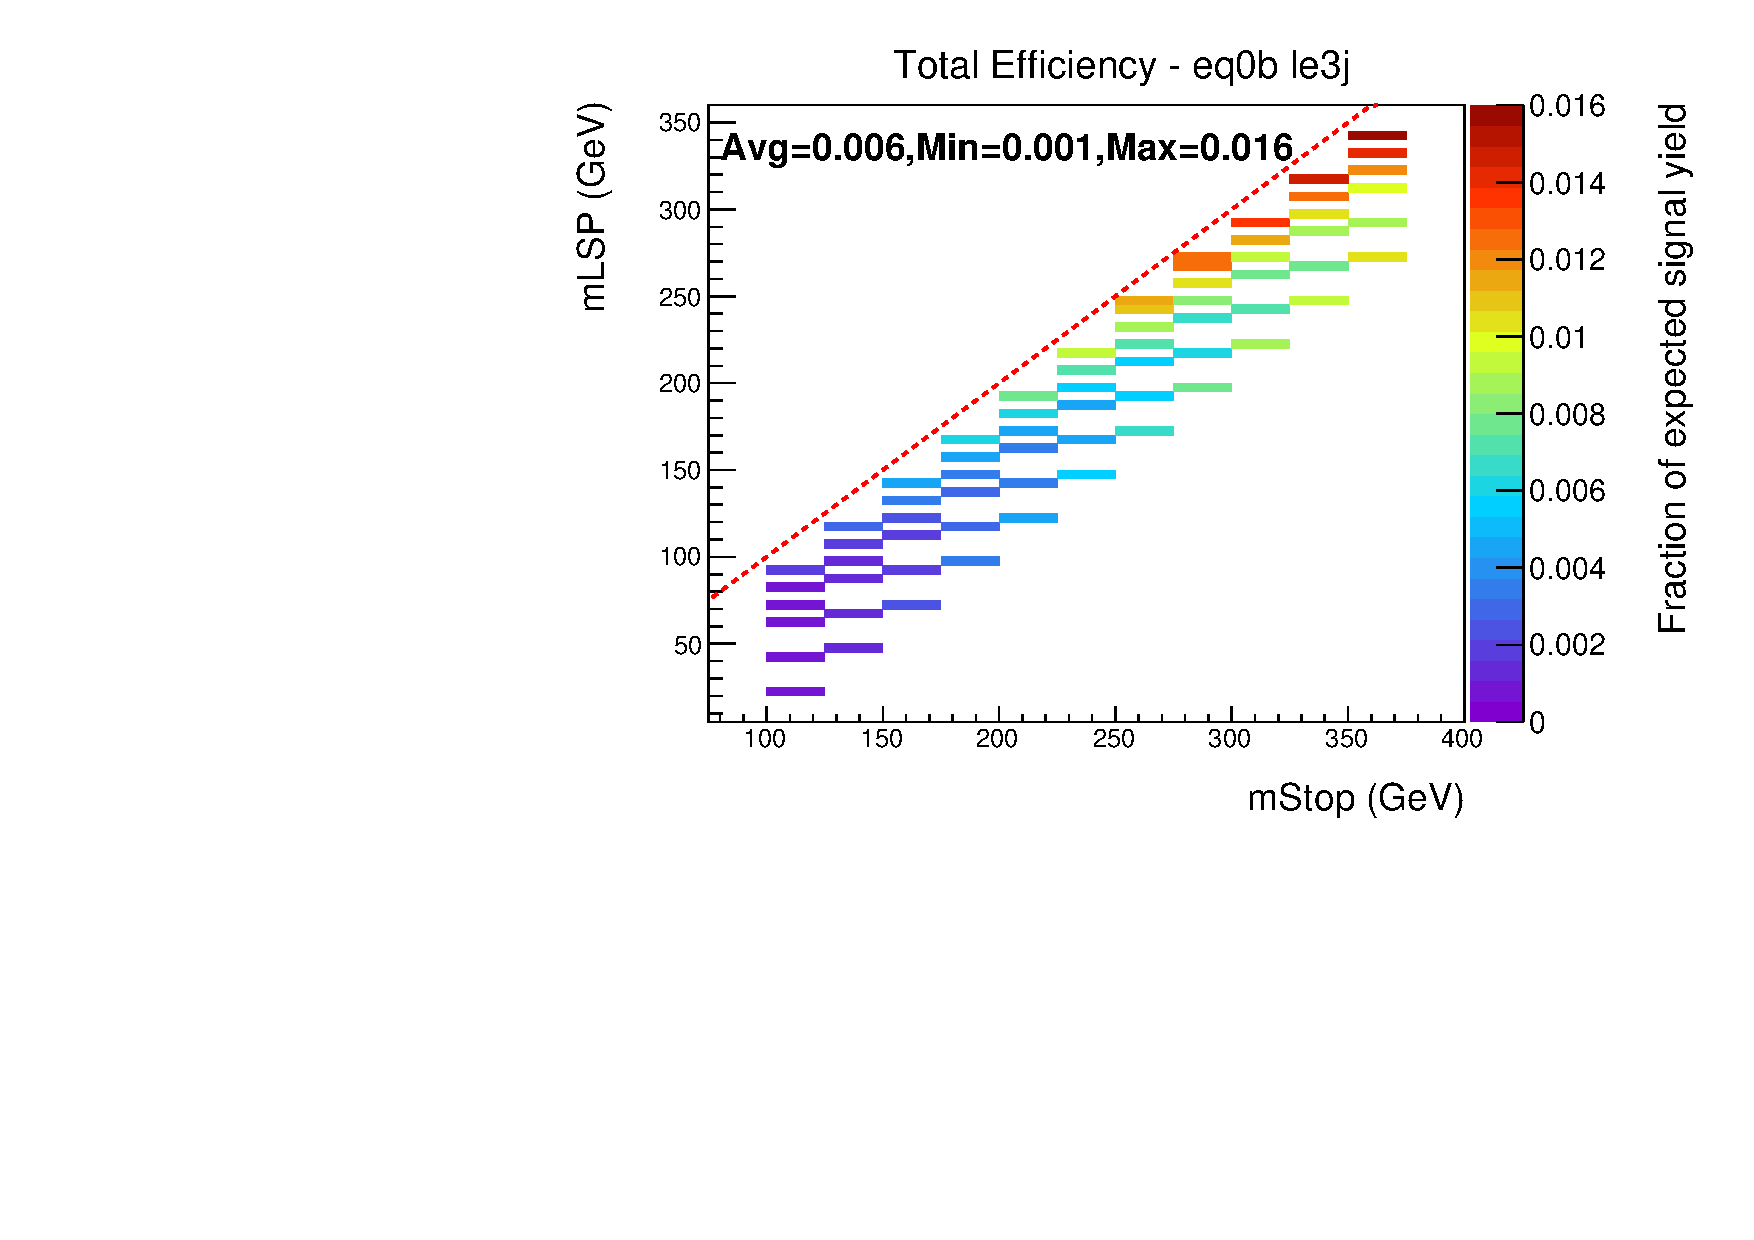
\includegraphics[width=\textwidth, trim=0 0 0 24, clip=true]{Figs/sms/t2cc/v24/T2cc_v24_had_eff_maps_eq0b_le3j_SITV.pdf}
    \caption{Signal region, (2--3,0)}
    \label{fig:t2cc_sig_eff_le3j_0b}
  \end{subfigure}
  \begin{subfigure}[b]{0.47\textwidth}
    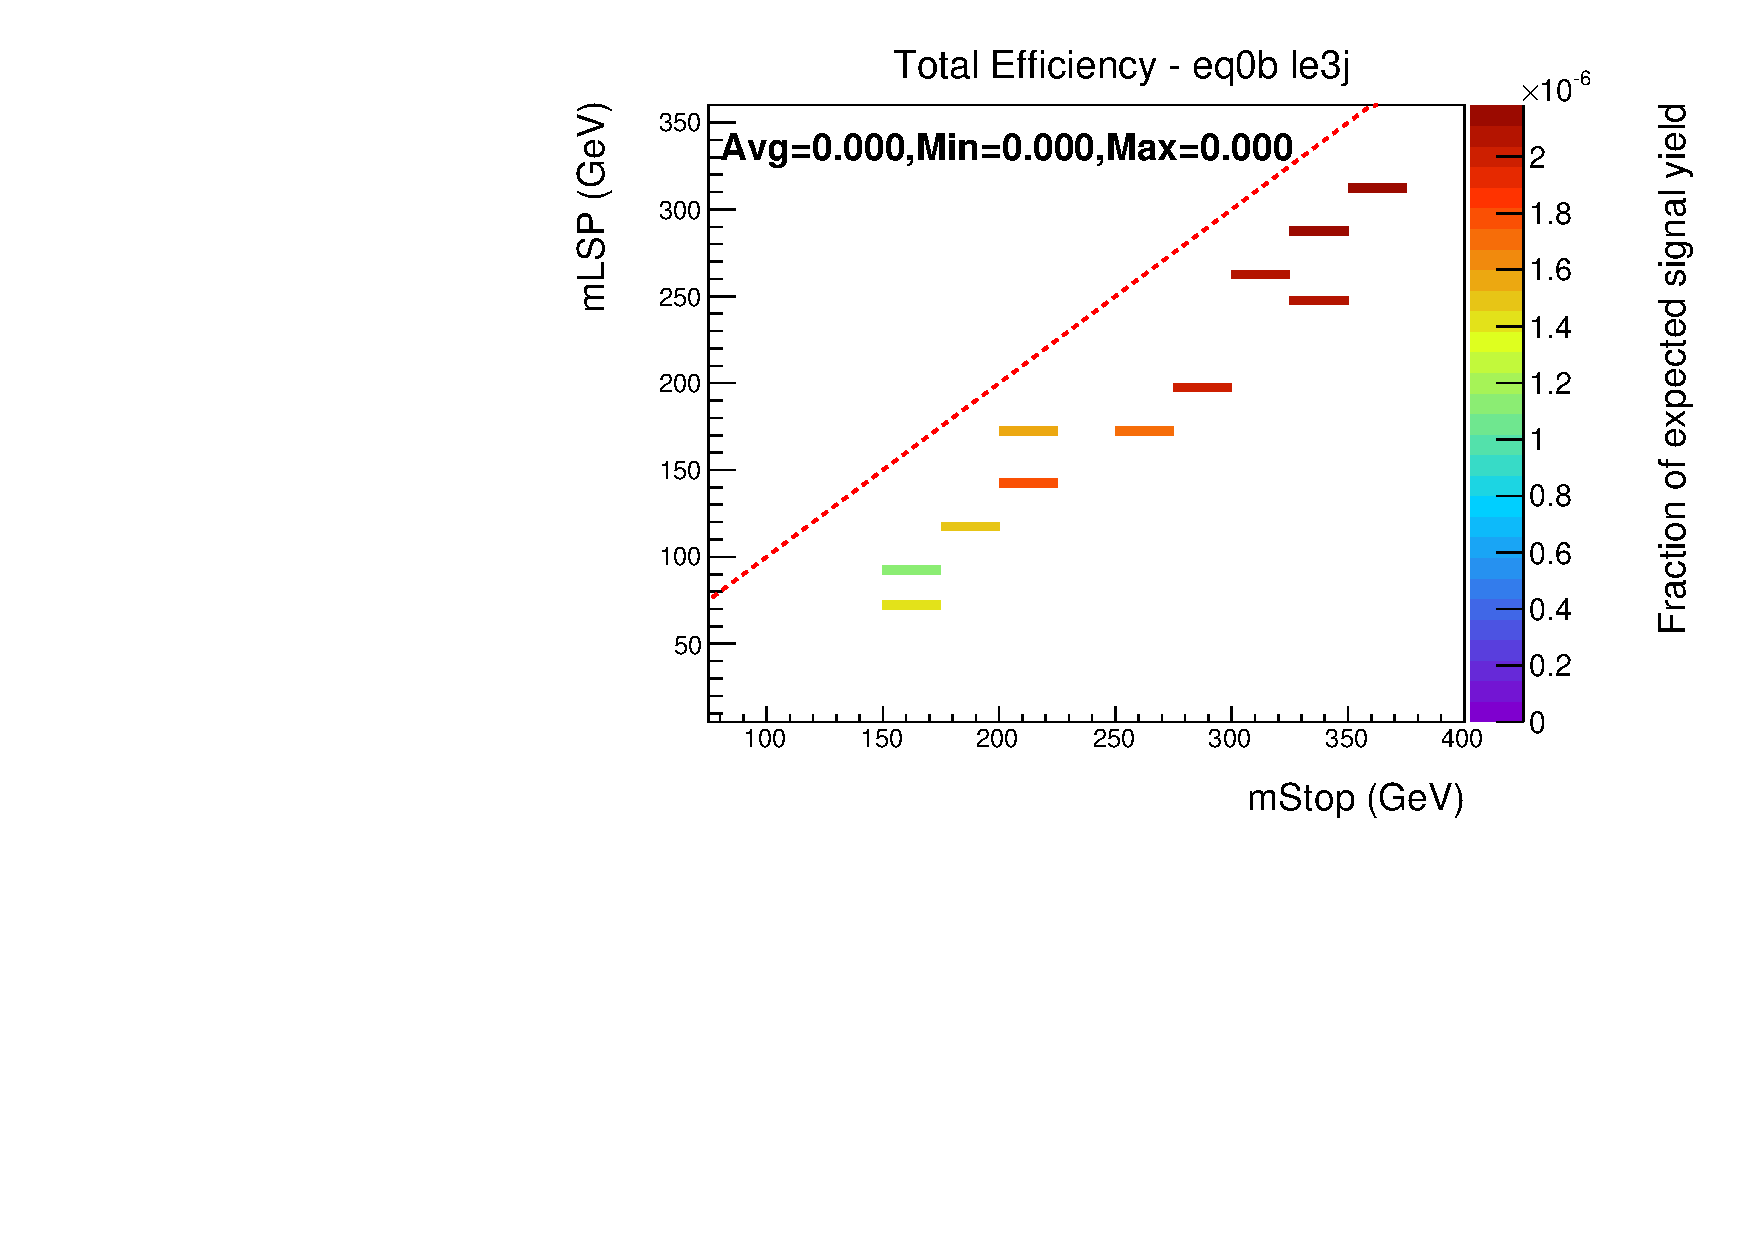
\includegraphics[width=\textwidth, trim=0 0 0 24, clip=true]{Figs/sms/t2cc/v24/T2cc_v24_muon_eff_maps_eq0b_le3j_SITV.pdf}
    \caption{\mj region, (2--3,0)}
    \label{fig:t2cc_mu_eff_le3j_0b}
  \end{subfigure} \\
  \begin{subfigure}[b]{0.47\textwidth}
    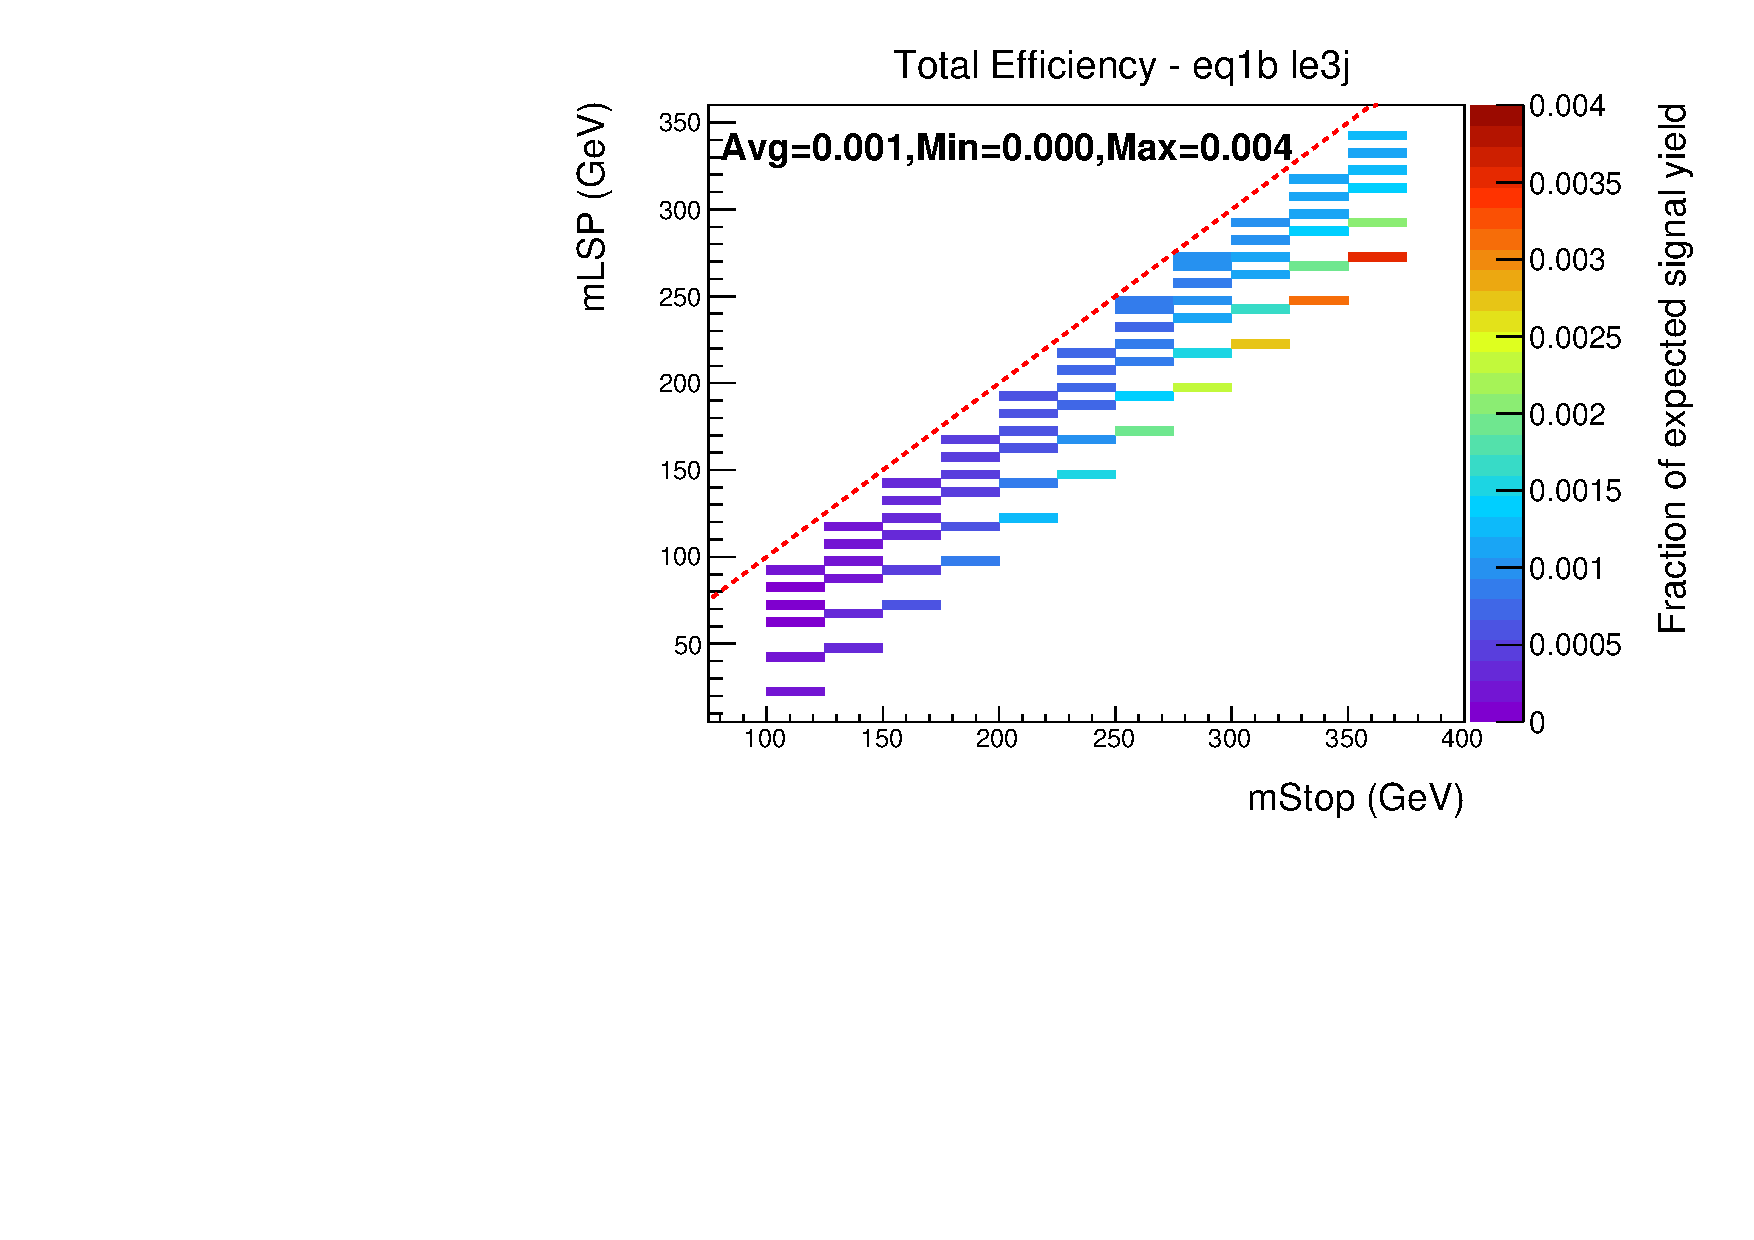
\includegraphics[width=\textwidth, trim=0 0 0 24, clip=true]{Figs/sms/t2cc/v24/T2cc_v24_had_eff_maps_eq1b_le3j_SITV.pdf}
    \caption{Signal region, (2--3,1)}
    \label{fig:t2cc_sig_eff_le3j_1b}
  \end{subfigure}
  \begin{subfigure}[b]{0.47\textwidth}
    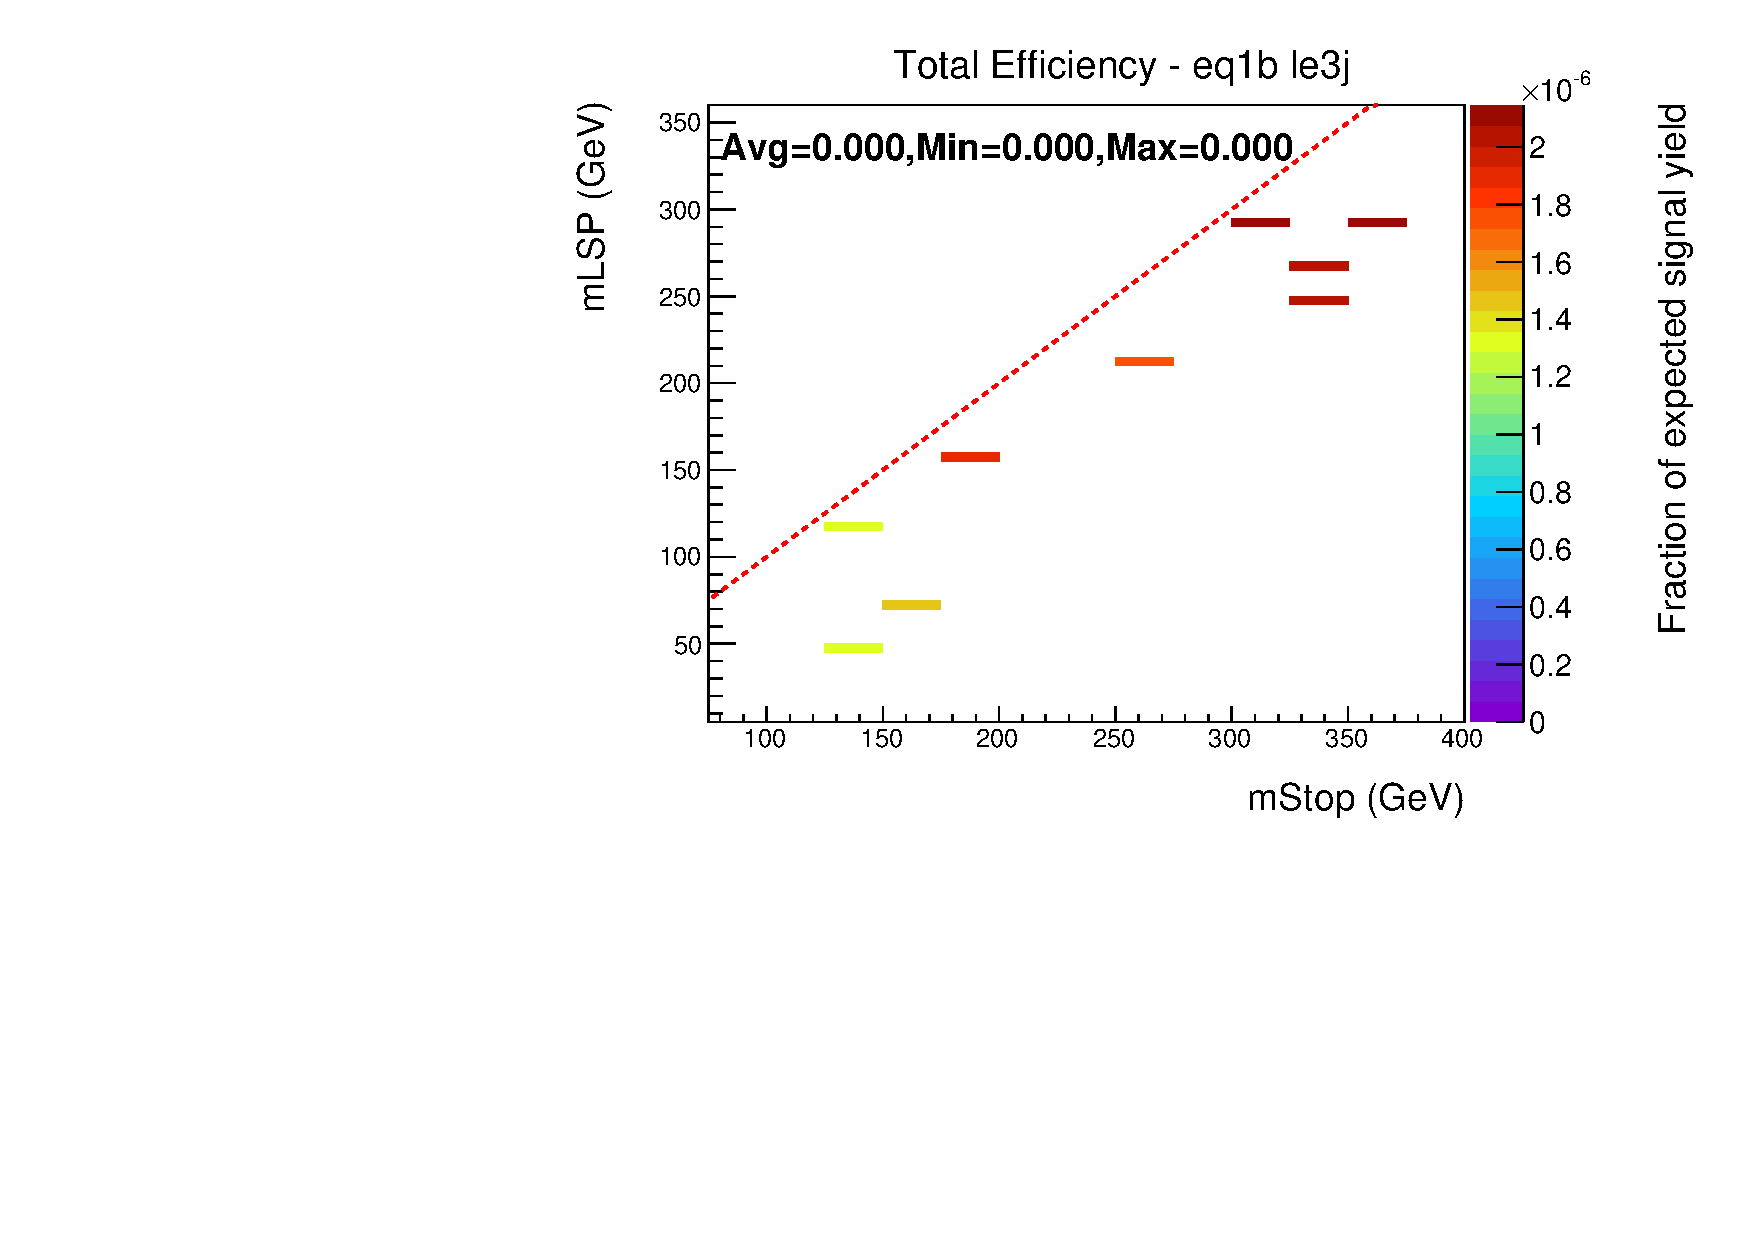
\includegraphics[width=\textwidth, trim=0 0 0 24, clip=true]{Figs/sms/t2cc/v24/T2cc_v24_muon_eff_maps_eq1b_le3j_SITV.pdf}
    \caption{\mj region, (2--3,1)}
    \label{fig:t2cc_mu_eff_le3j_1b}
  \end{subfigure} \\
  \begin{subfigure}[b]{0.47\textwidth}
    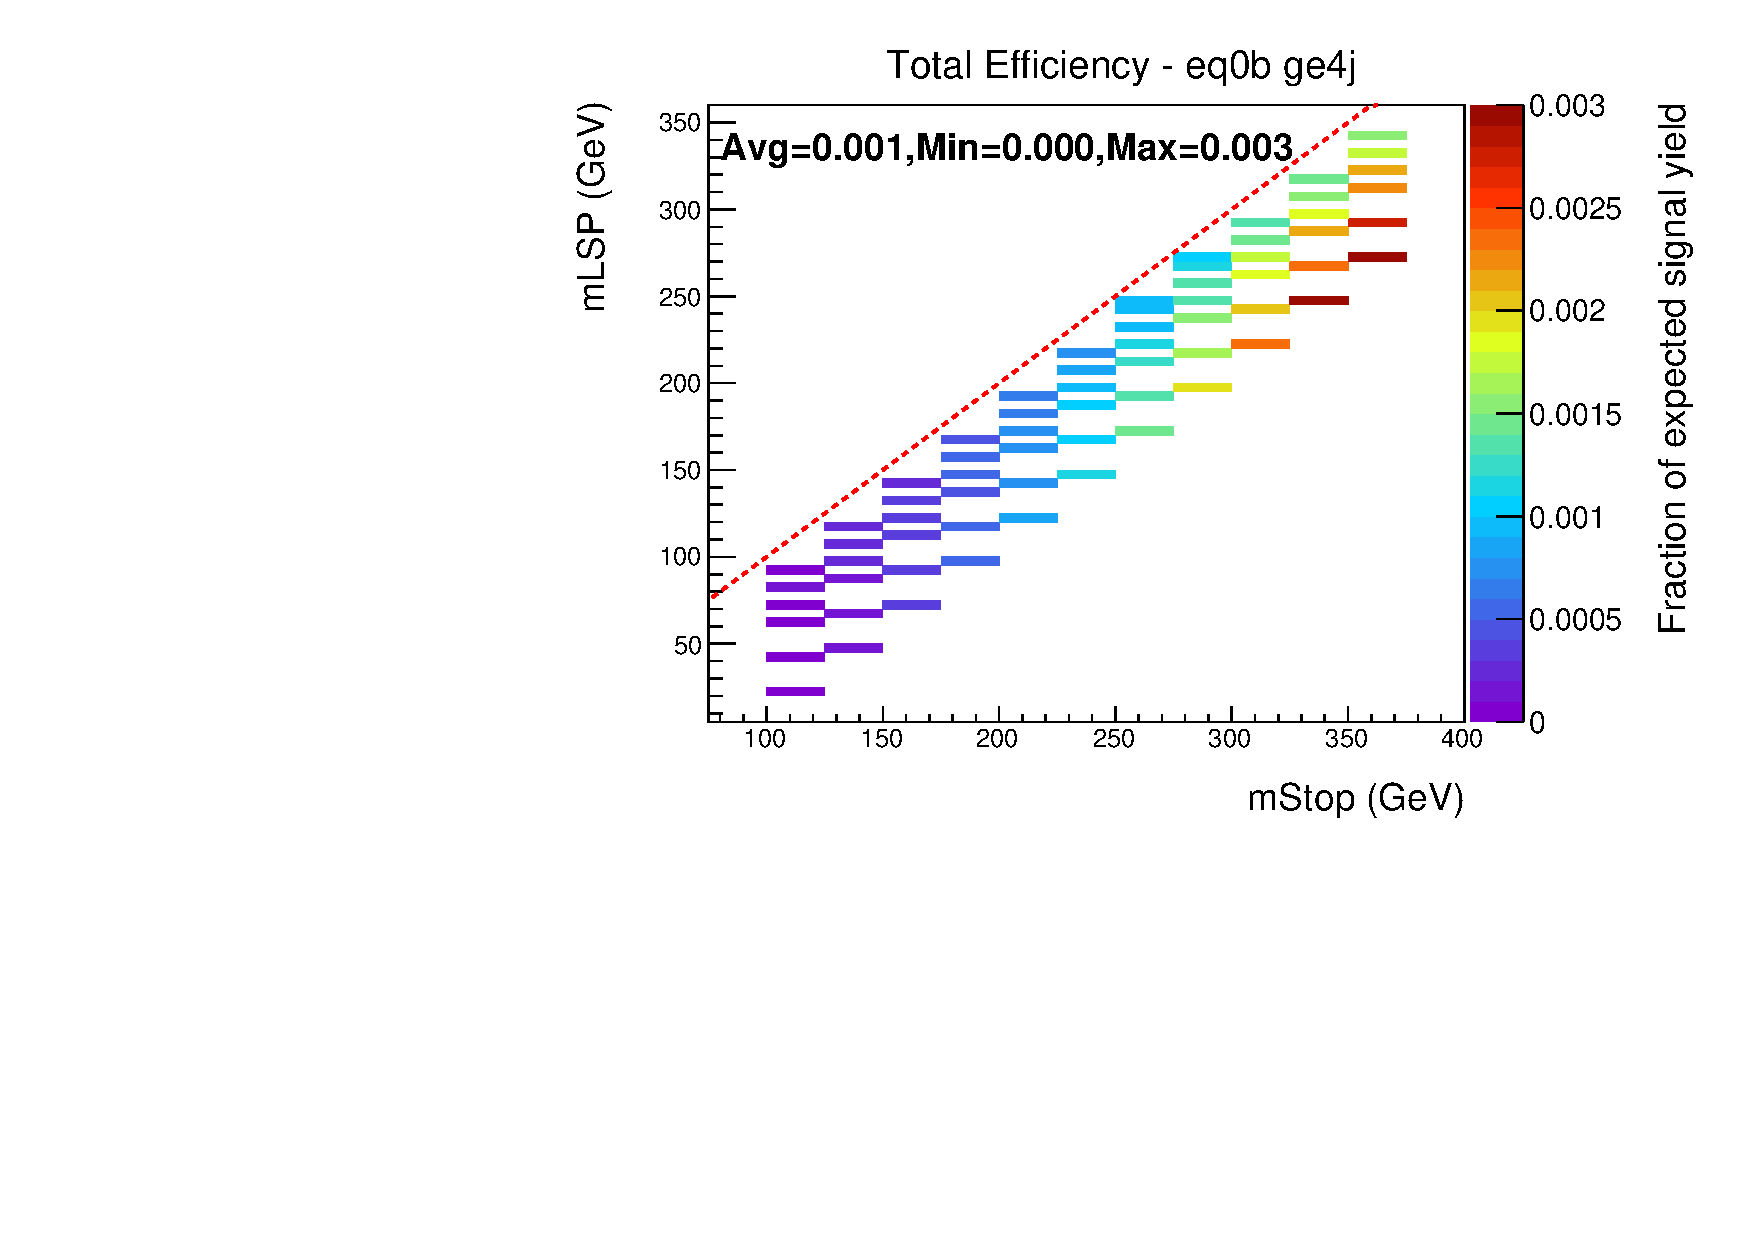
\includegraphics[width=\textwidth, trim=0 0 0 24, clip=true]{Figs/sms/t2cc/v24/T2cc_v24_had_eff_maps_eq0b_ge4j_SITV.pdf}
    \caption{Signal region, ($\geq 4$,0)}
    \label{fig:t2cc_sig_eff_ge4j_0b}
  \end{subfigure}
  \begin{subfigure}[b]{0.47\textwidth}
    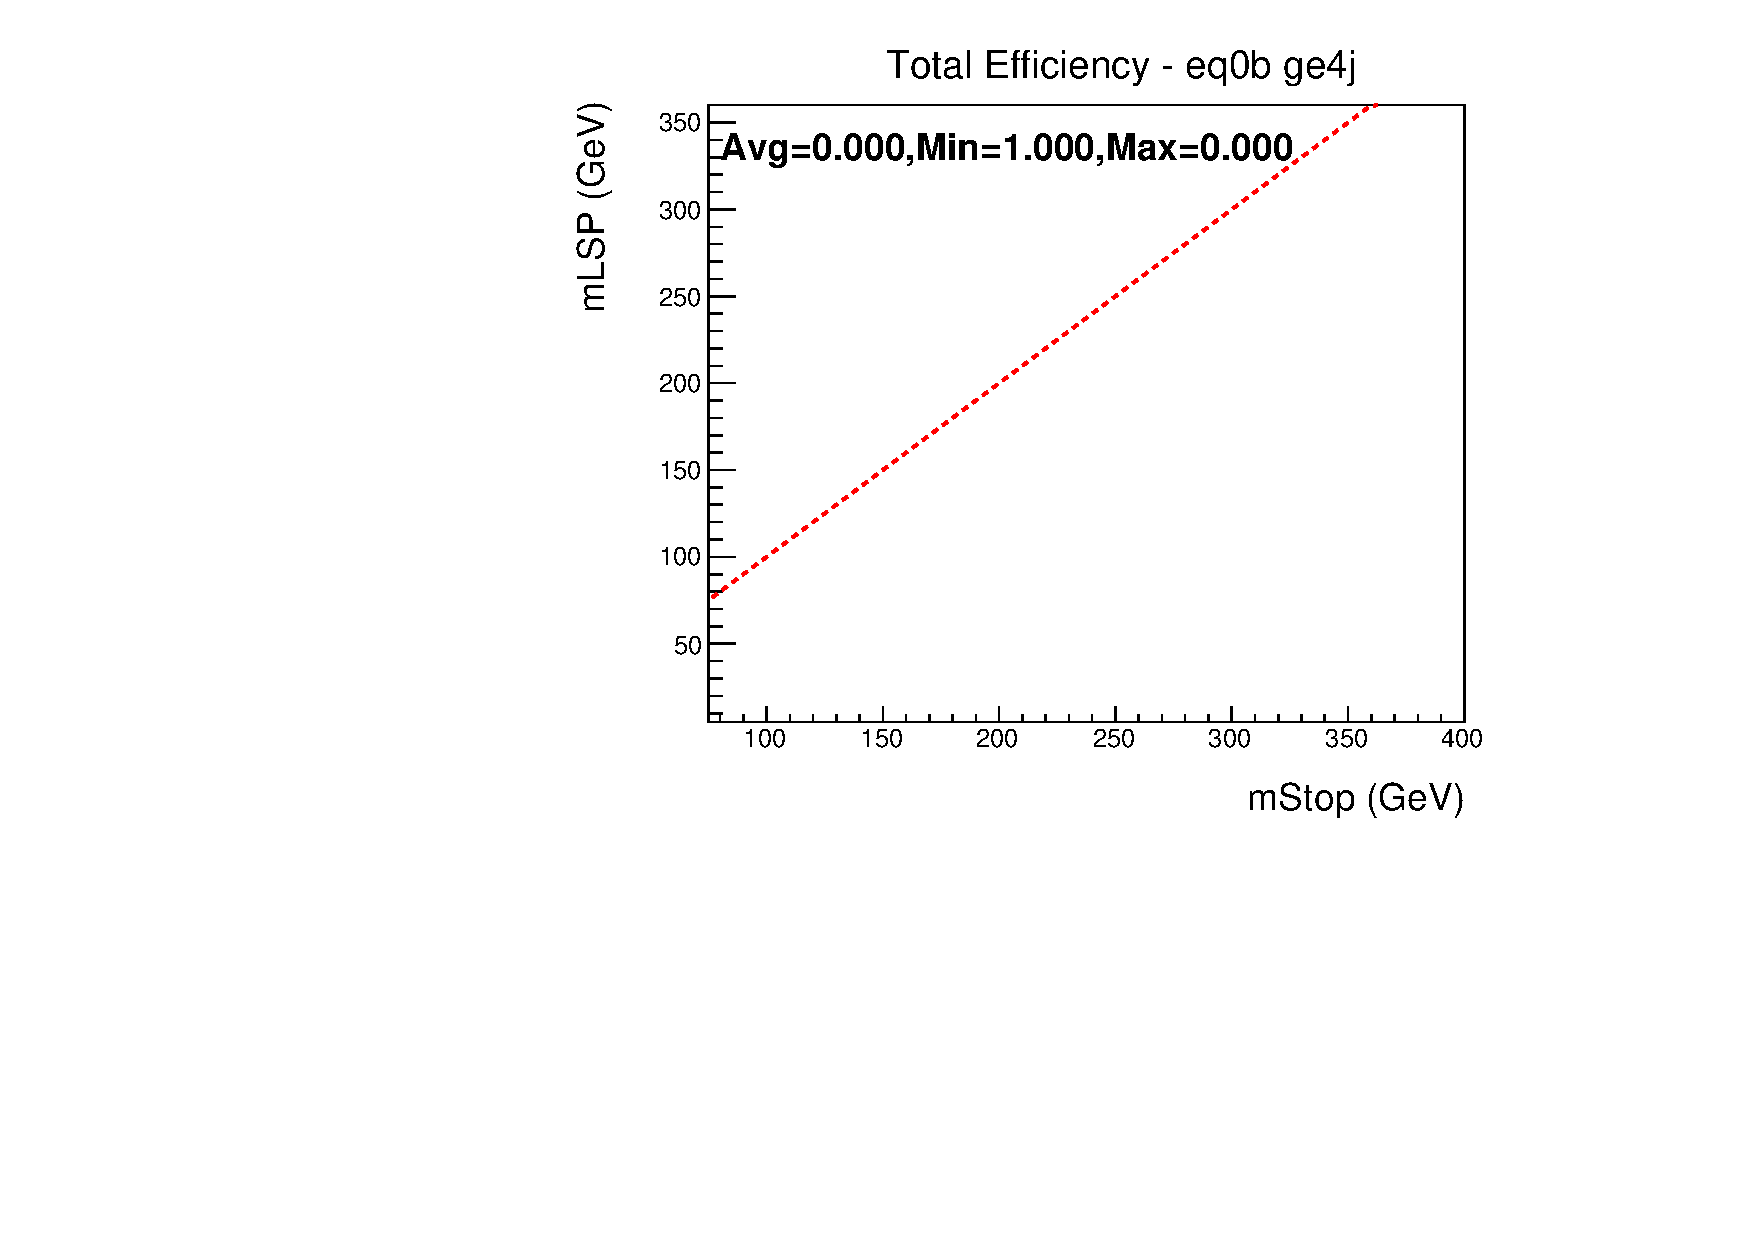
\includegraphics[width=\textwidth, trim=0 0 0 24, clip=true]{Figs/sms/t2cc/v24/T2cc_v24_muon_eff_maps_eq0b_ge4j_SITV.pdf}
    \caption{\mj region, ($\geq 4$,0)}
    \label{fig:t2cc_mu_eff_ge4j_0b}
  \end{subfigure} \\
  \begin{subfigure}[b]{0.47\textwidth}
    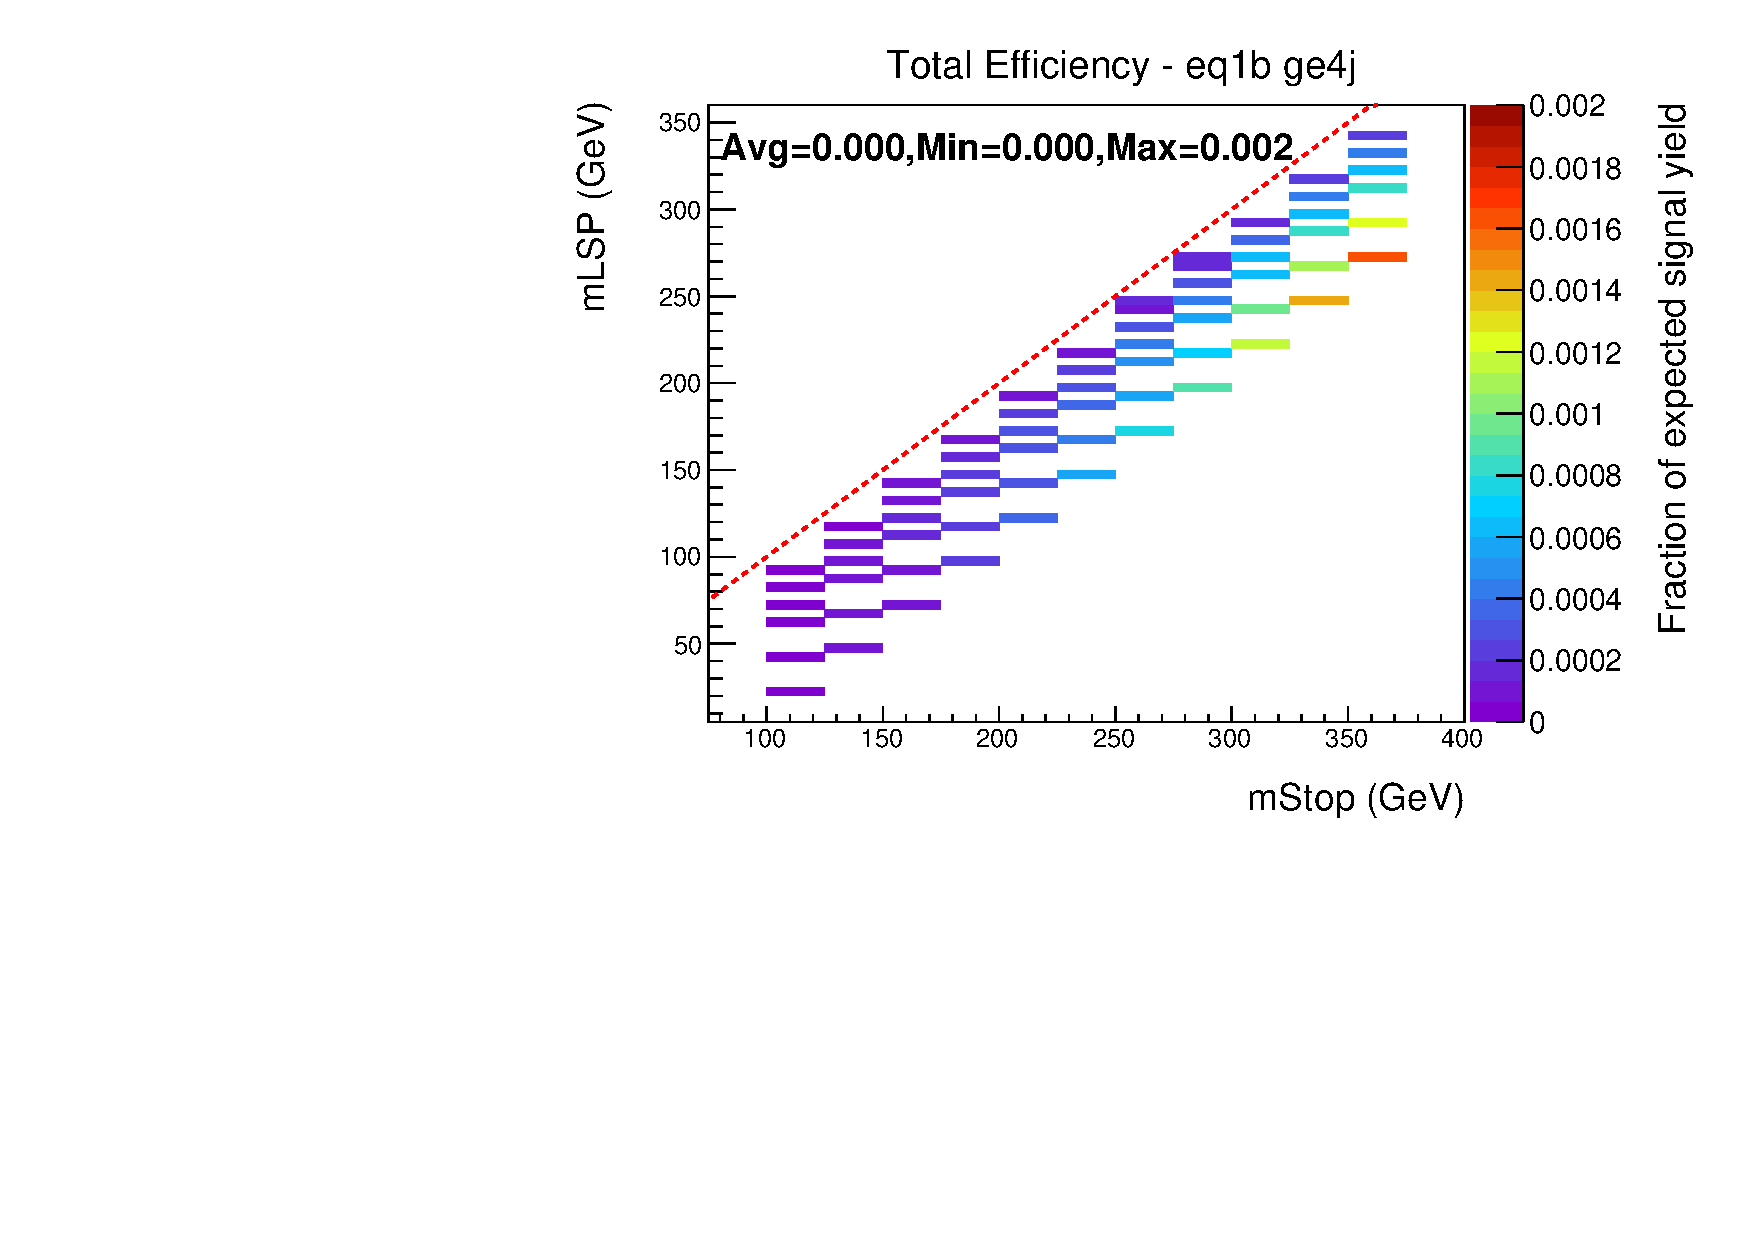
\includegraphics[width=\textwidth, trim=0 0 0 24, clip=true]{Figs/sms/t2cc/v24/T2cc_v24_had_eff_maps_eq1b_ge4j_SITV.pdf}
    \caption{Signal region, ($\geq 4$,1)}
    \label{fig:t2cc_sig_eff_ge4j_1b}
  \end{subfigure}
  \begin{subfigure}[b]{0.47\textwidth}
    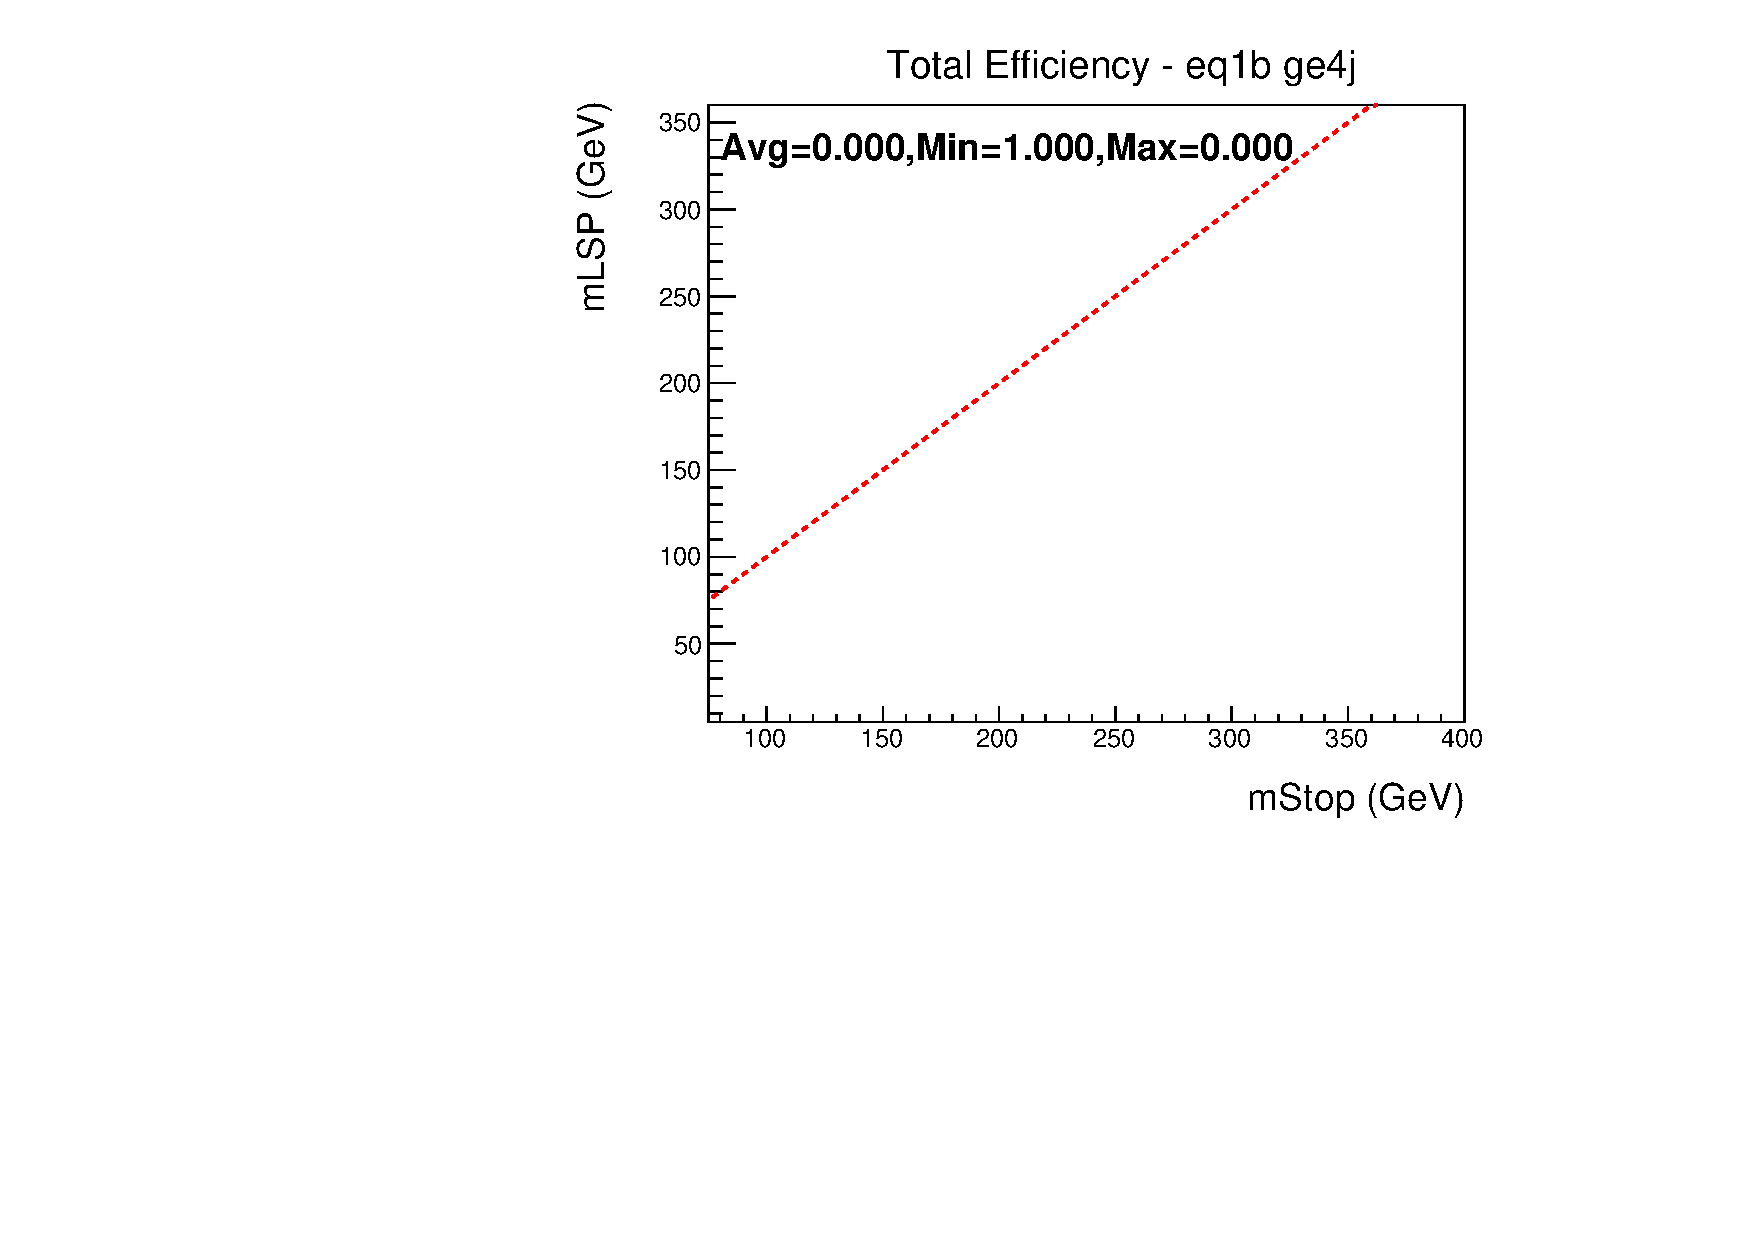
\includegraphics[width=\textwidth, trim=0 0 0 24, clip=true]{Figs/sms/t2cc/v24/T2cc_v24_muon_eff_maps_eq1b_ge4j_SITV.pdf}
    \caption{\mj region, ($\geq 4$,1)}
    \label{fig:t2cc_mu_eff_ge4j_1b}
  \end{subfigure} \\
  \caption{Signal efficiency times acceptance for the \Ttwocc simplified, for 
  the hadronic selection (left) and the \mj selection (right), shown for the 
  four most sensitive analysis categories with an inclusive selection on \HT.}
  \label{fig:t2cc_eff}
\end{figure}

% \begin{figure}[h!]
%   \centering
%   \begin{subfigure}[b]{0.6\textwidth}
%     \includegraphics[width=\textwidth, trim=0 0 0 30, clip=true]{Figs/sms/t2cc/v24/T2cc_v24_sig_inj_250_170.pdf}
%     \caption{$m_{\sTop} = 250\gev, m_{\rm LSP} = 170\gev$}
%     \label{fig:t2cc_sig_inj_dm80}
%   \end{subfigure}
%   \begin{subfigure}[b]{0.6\textwidth}
%     \includegraphics[width=\textwidth, trim=0 0 0 30, clip=true]{Figs/sms/t2cc/v24/T2cc_v24_sig_inj_250_240.pdf}
%     \caption{$m_{\sTop} = 250\gev, m_{\rm LSP} = 240\gev$}
%     \label{fig:t2cc_sig_inj_dm10}
%   \end{subfigure}
%   \caption{balls}
%   \label{fig:}
% \end{figure}

\subsection{T2\_4body}
\label{sec:t2degen_eff}

The signal efficiency times acceptance distributions for the \texttt{T2degen} model,
\Ttwodegen, are shown 
in figure~\ref{fig:t2_4body_eff} in the four most sensitive analysis categories,
with an inclusive \HT selection, both for the hadronic and \mj selections. There
are strong similarities with those shown earlier for the \texttt{T2cc} model, 
both in magnitude and distribution about the plane. At small values of \deltam, 
given that the entire SUSY decay system becomes invisible due to a lack of 
kinematic phase space, both models show very similar efficiencies, where 
acceptance is almost entirely due to hard ISR jets within acceptance. There is a
significant difference however, when a b-tagged jet is required, for example in 
the \njlow, \nb=1 category, where the presence of a jet originating from a real 
b quark improves acceptance, particularly away from the diagonal where this jet 
would be more likely to pass analysis thresholds. Less significant are the 
efficiencies seen in the \njhigh categories, given the larger number of final 
state object, each requiring a share of the energy originating from the mass 
splitting of the mother and daughter sparticles.

Also of note is the increase in signal contamination observed in the \mj 
selection, due to the presence of $f\bar{f}$ in the decay chain, potentially 
giving leptons in the final state.

% should be v16!!
\begin{figure}[ht!]
  \centering
  \begin{subfigure}[b]{0.47\textwidth}
    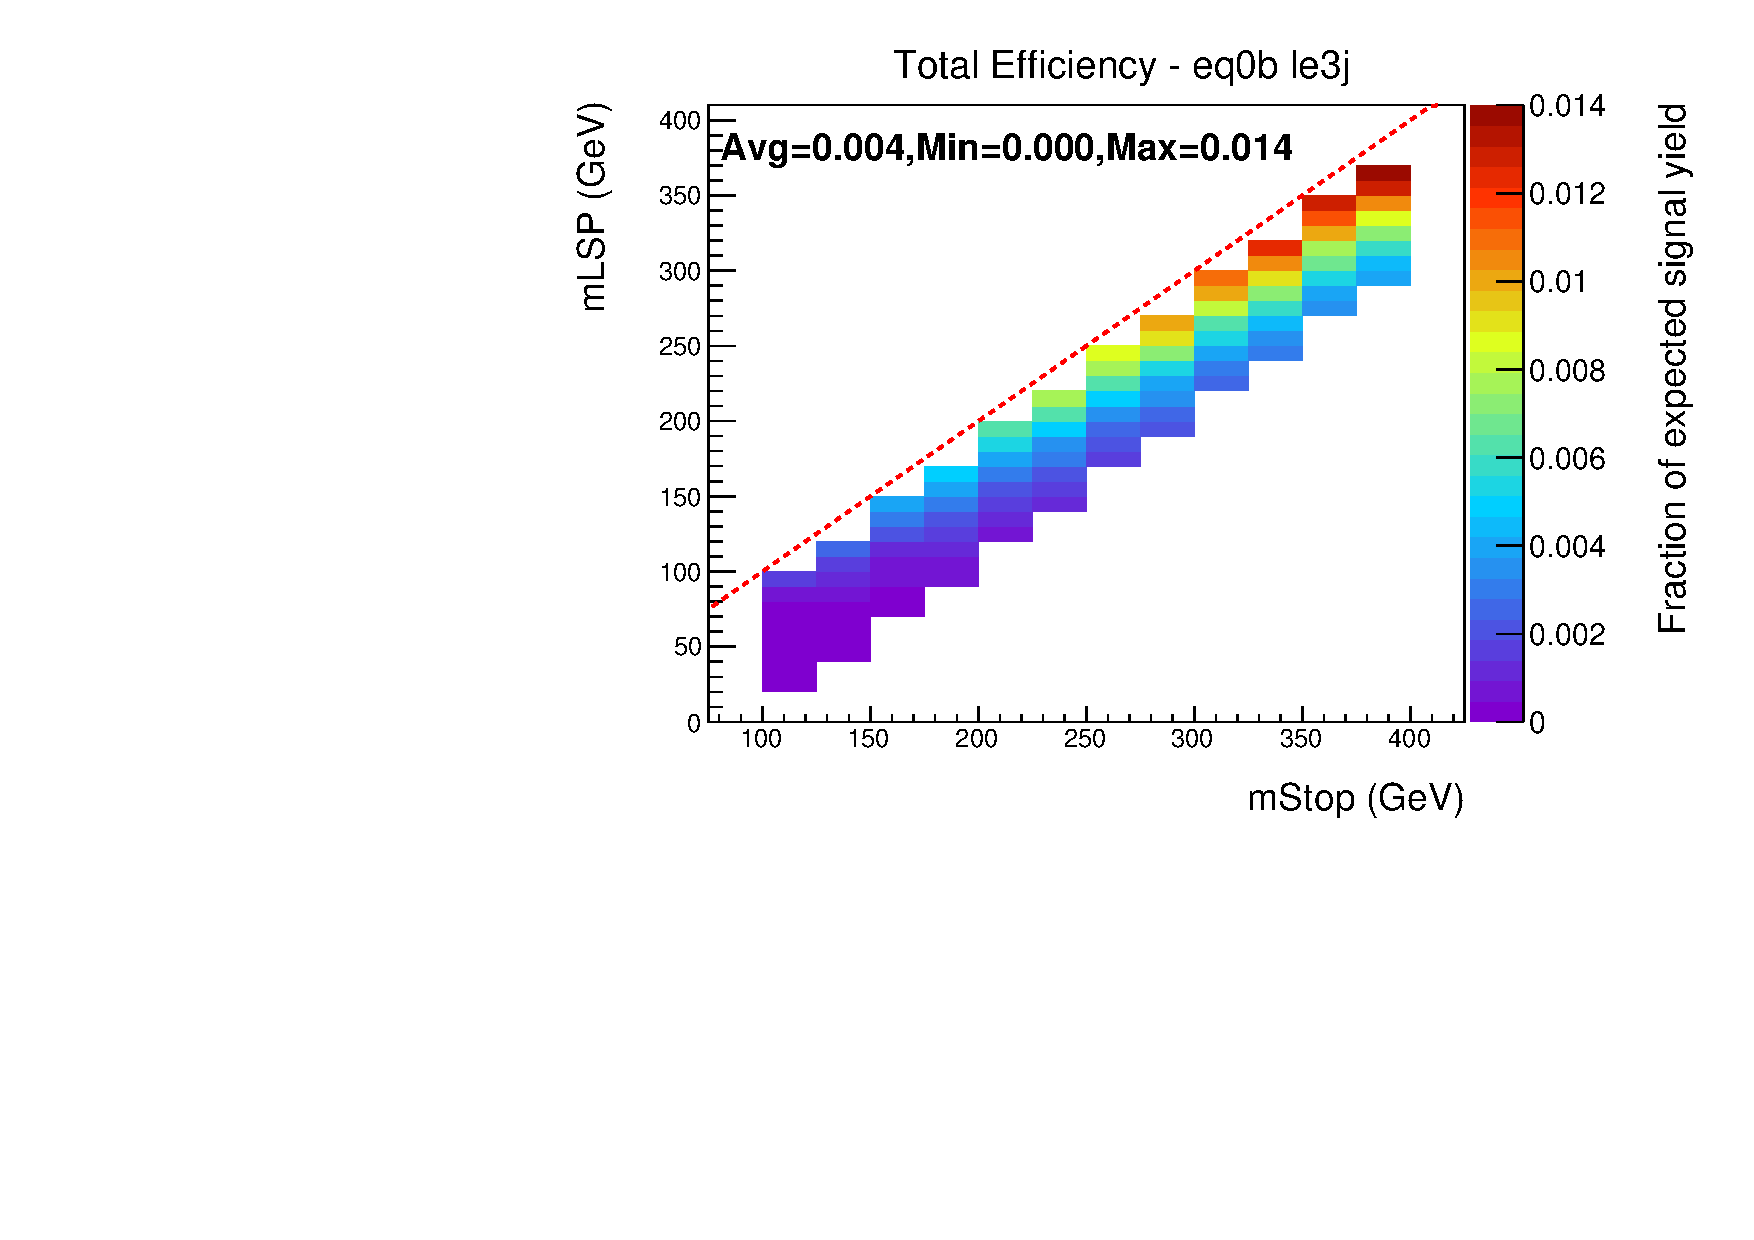
\includegraphics[width=\textwidth, trim=0 0 0 24, clip=true]{Figs/sms/t2degen/v5/T2_4body_v5_had_eff_maps_eq0b_le3j_SITV.pdf}
    \caption{Signal region, (2--3,0)}
    \label{fig:t2_4body_sig_eff_le3j_0b}
  \end{subfigure}
  \begin{subfigure}[b]{0.47\textwidth}
    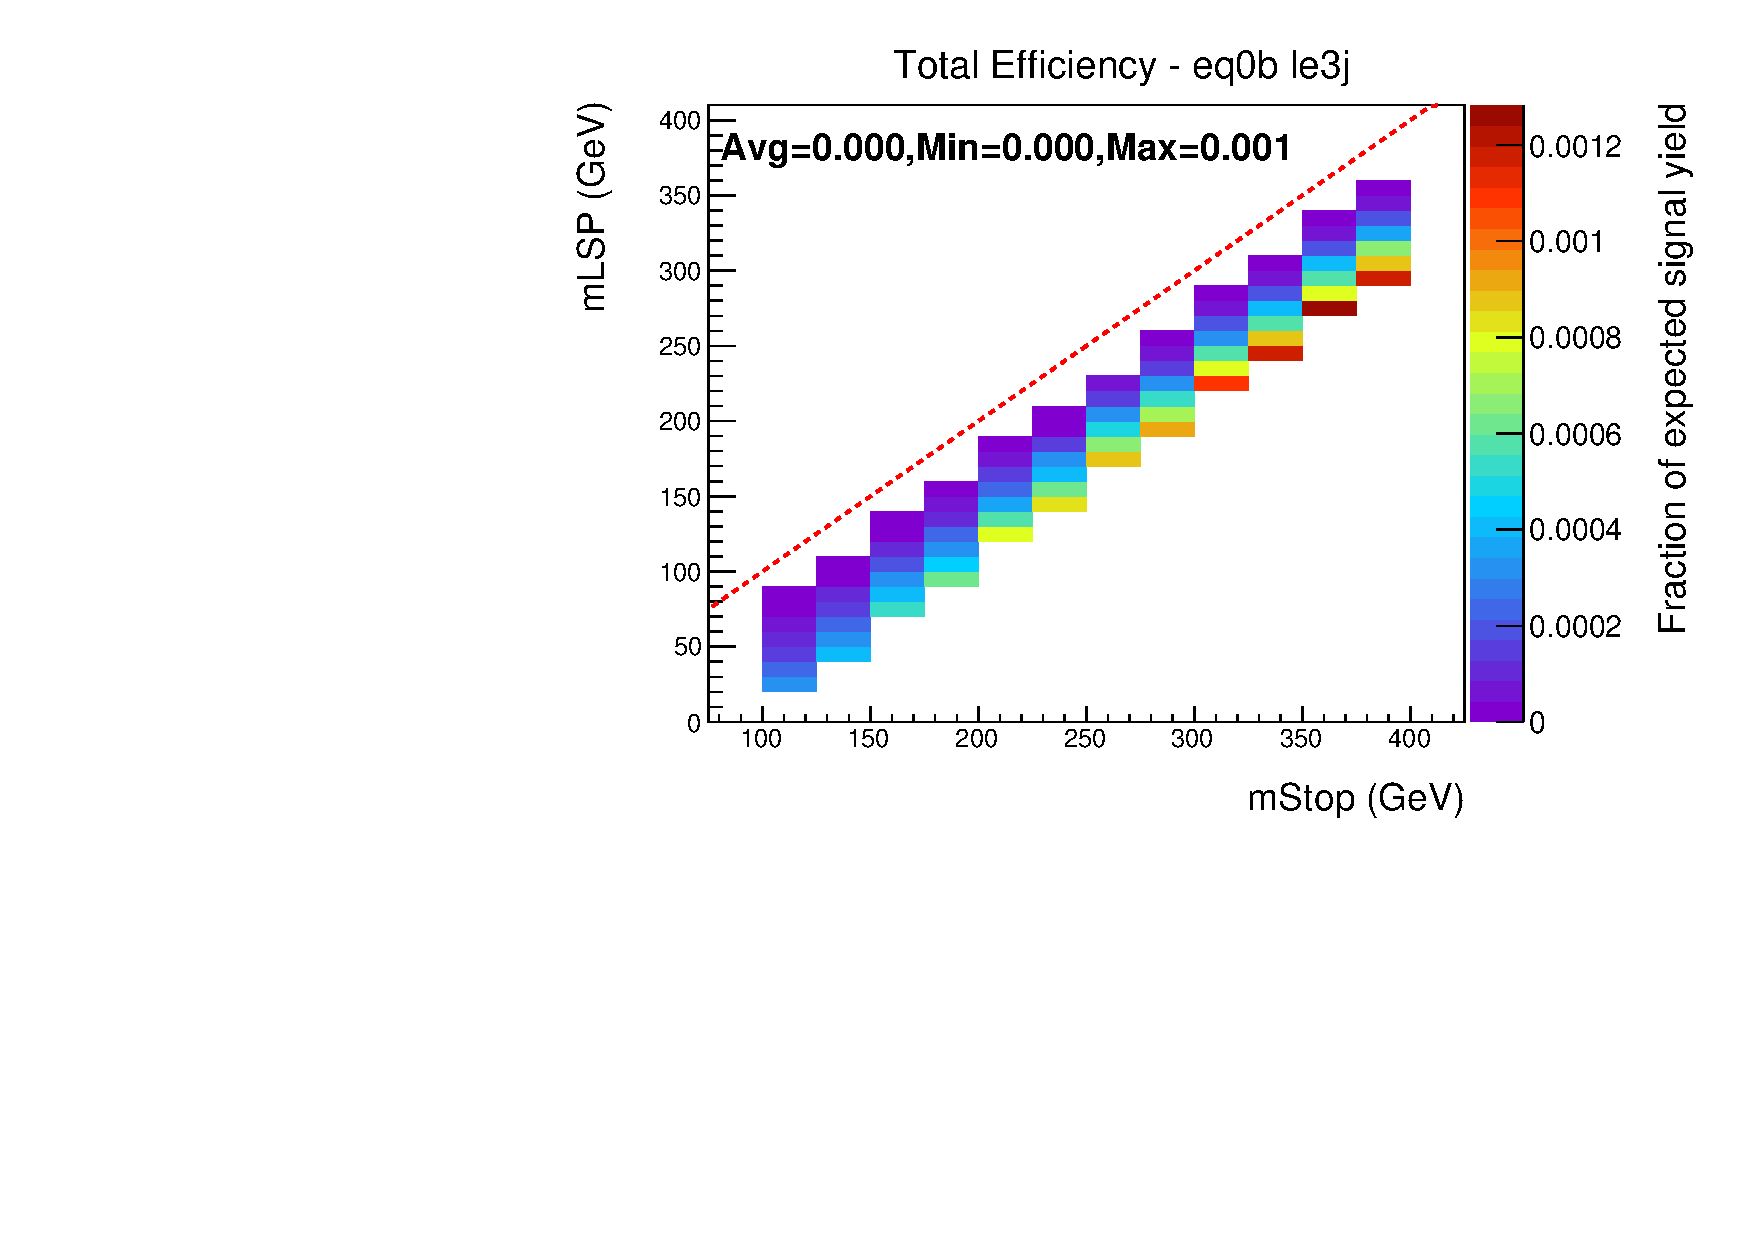
\includegraphics[width=\textwidth, trim=0 0 0 24, clip=true]{Figs/sms/t2degen/v5/T2_4body_v5_muon_eff_maps_eq0b_le3j_SITV.pdf}
    \caption{\mj region, (2--3,0)}
    \label{fig:t2_4body_mu_eff_le3j_0b}
  \end{subfigure} \\
  \begin{subfigure}[b]{0.47\textwidth}
    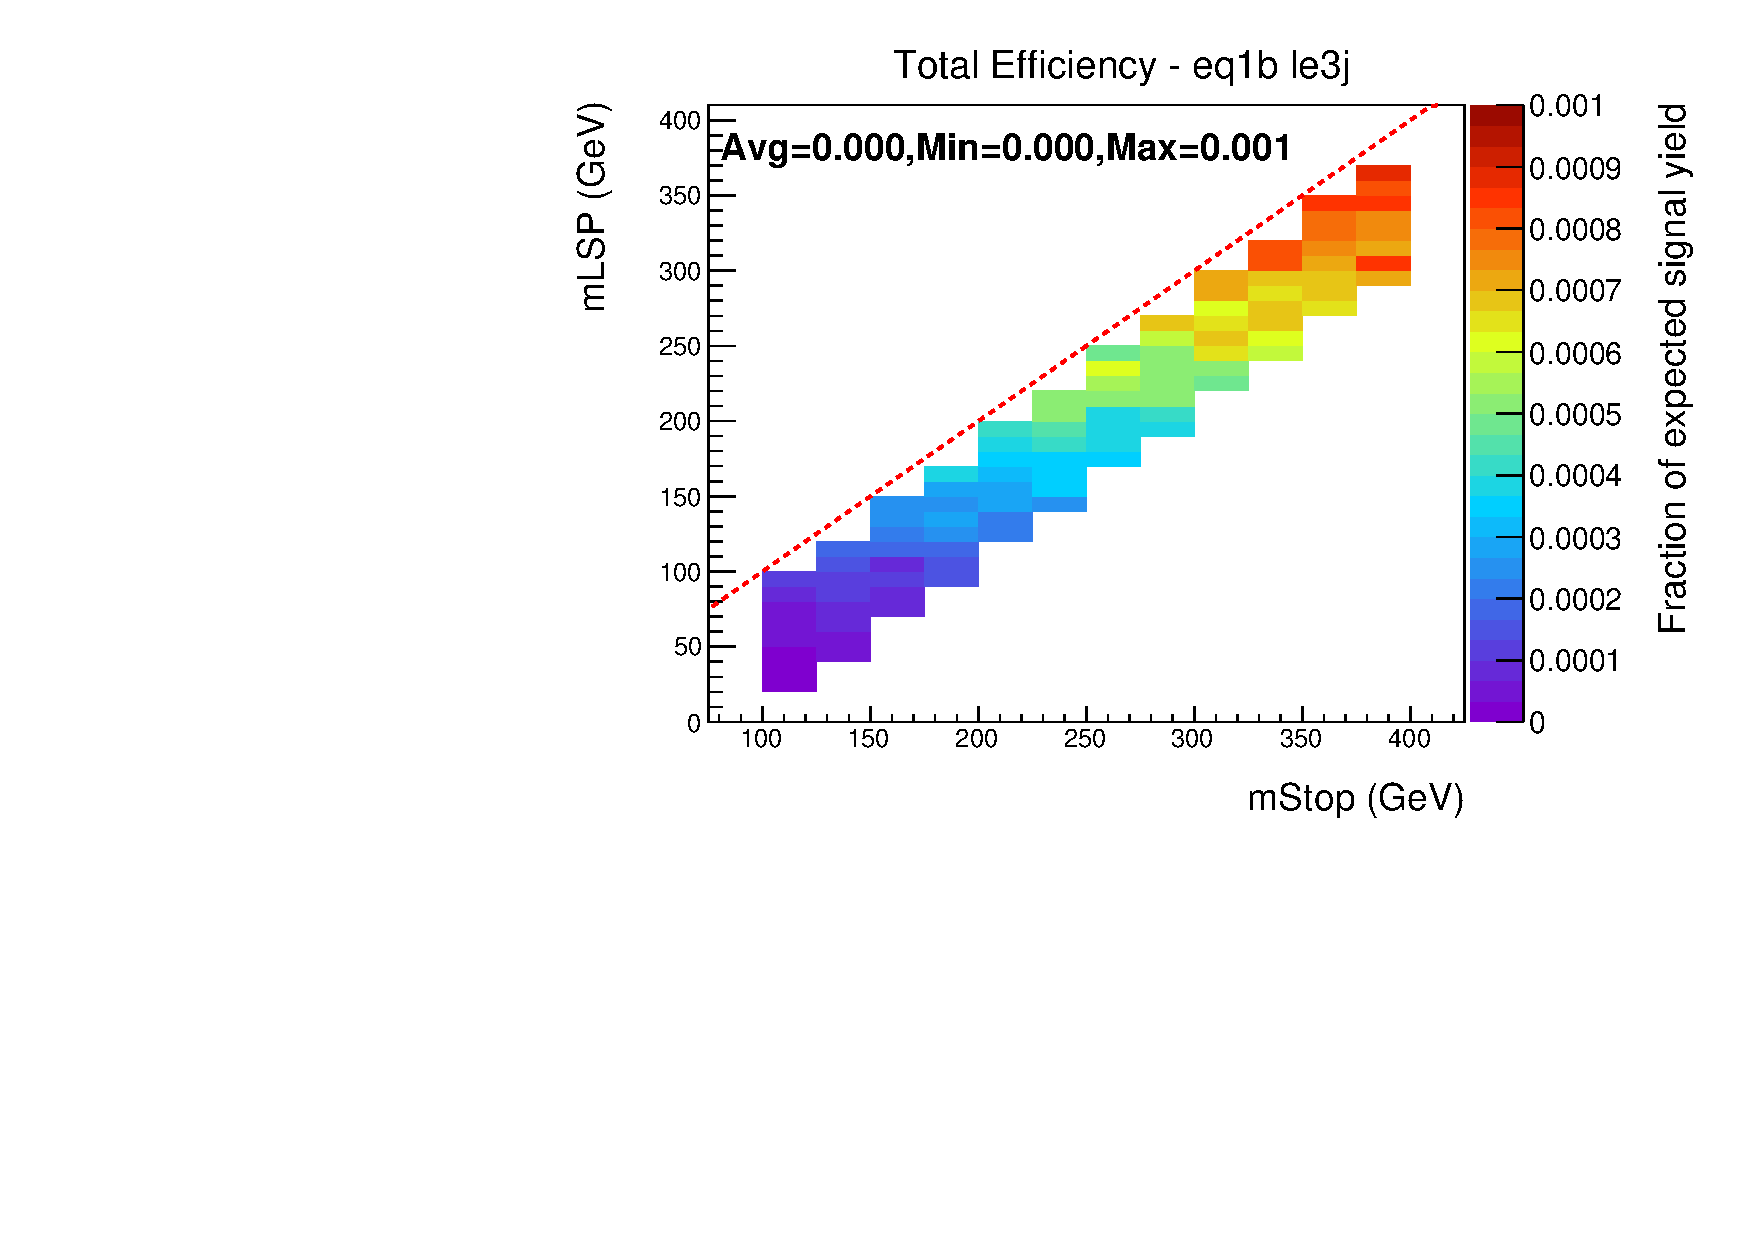
\includegraphics[width=\textwidth, trim=0 0 0 24, clip=true]{Figs/sms/t2degen/v5/T2_4body_v5_had_eff_maps_eq1b_le3j_SITV.pdf}
    \caption{Signal region, (2--3,1)}
    \label{fig:t2_4body_sig_eff_le3j_1b}
  \end{subfigure}
  \begin{subfigure}[b]{0.47\textwidth}
    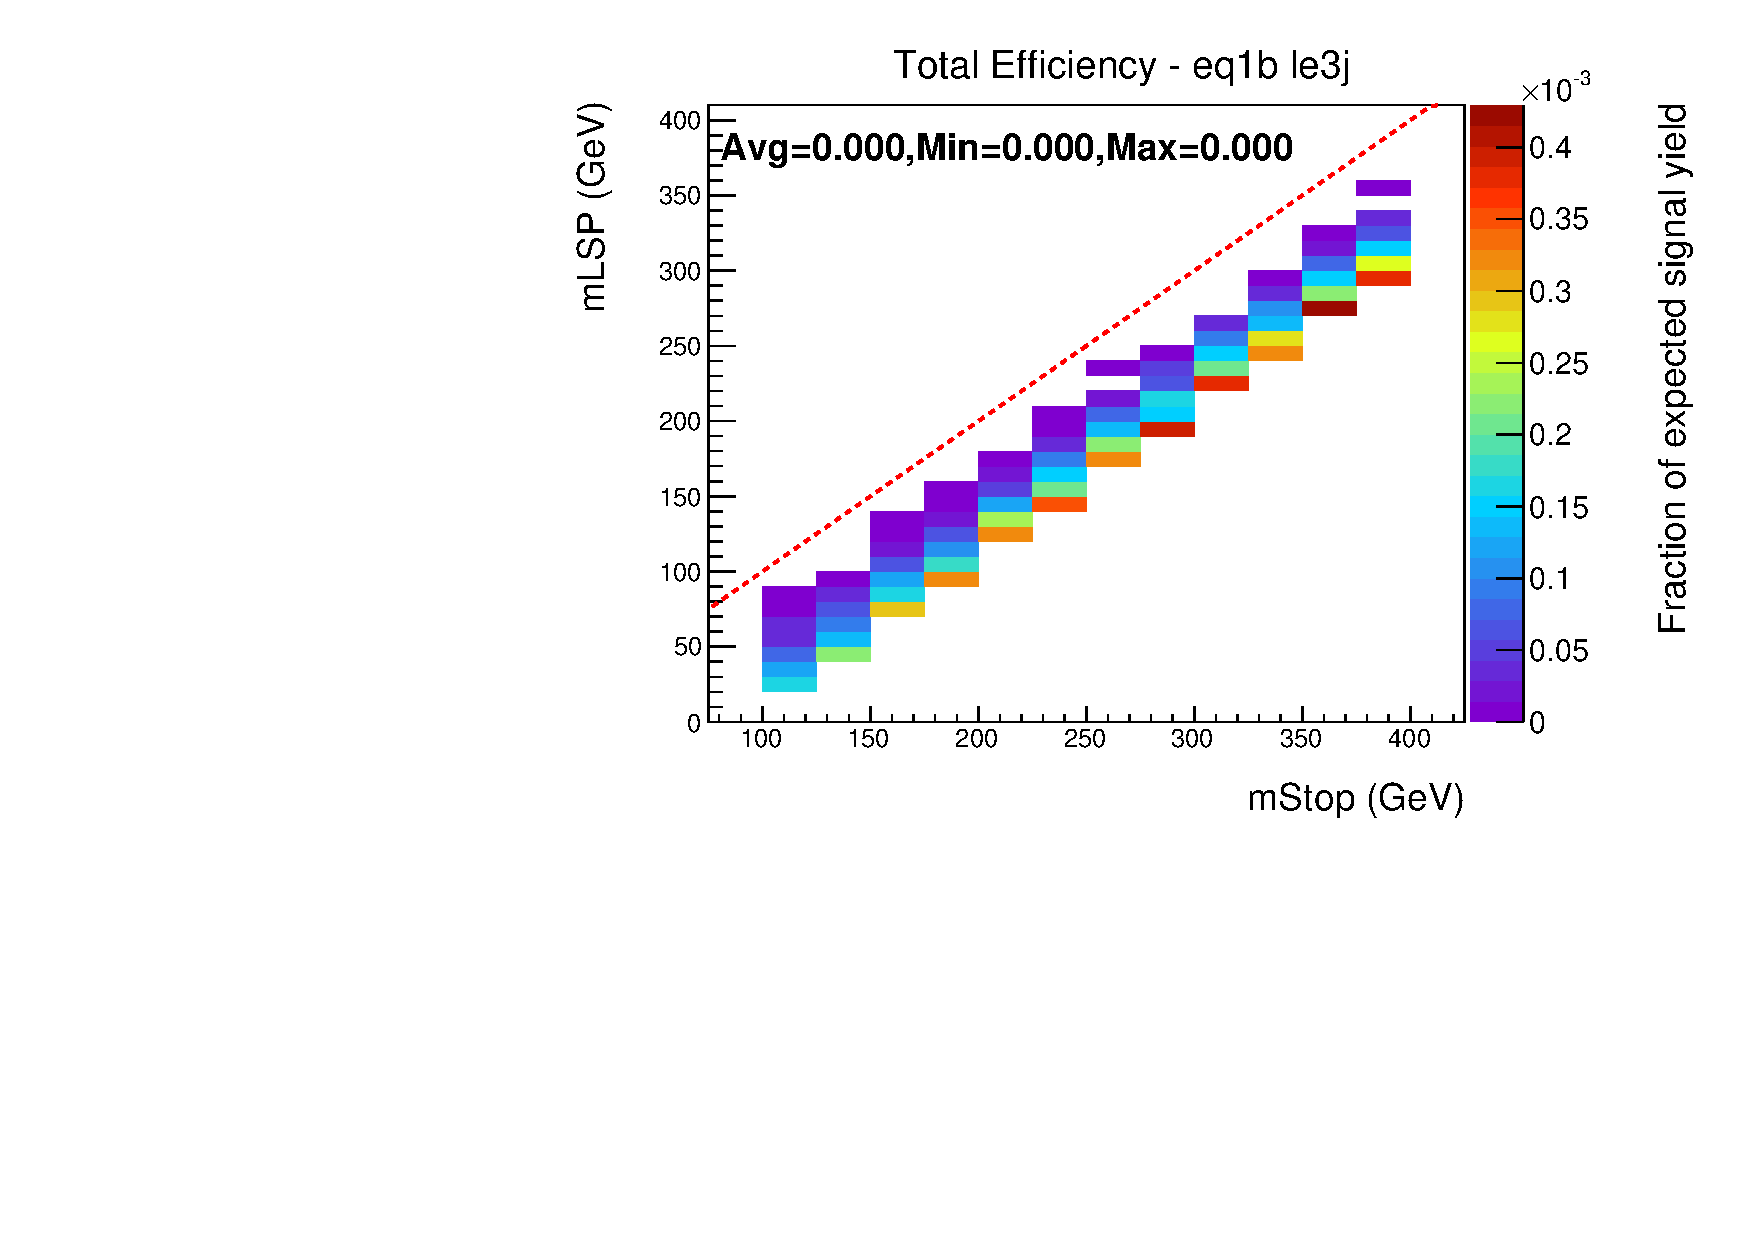
\includegraphics[width=\textwidth, trim=0 0 0 24, clip=true]{Figs/sms/t2degen/v5/T2_4body_v5_muon_eff_maps_eq1b_le3j_SITV.pdf}
    \caption{\mj region, (2--3,1)}
    \label{fig:t2_4body_mu_eff_le3j_1b}
  \end{subfigure} \\
  \begin{subfigure}[b]{0.47\textwidth}
    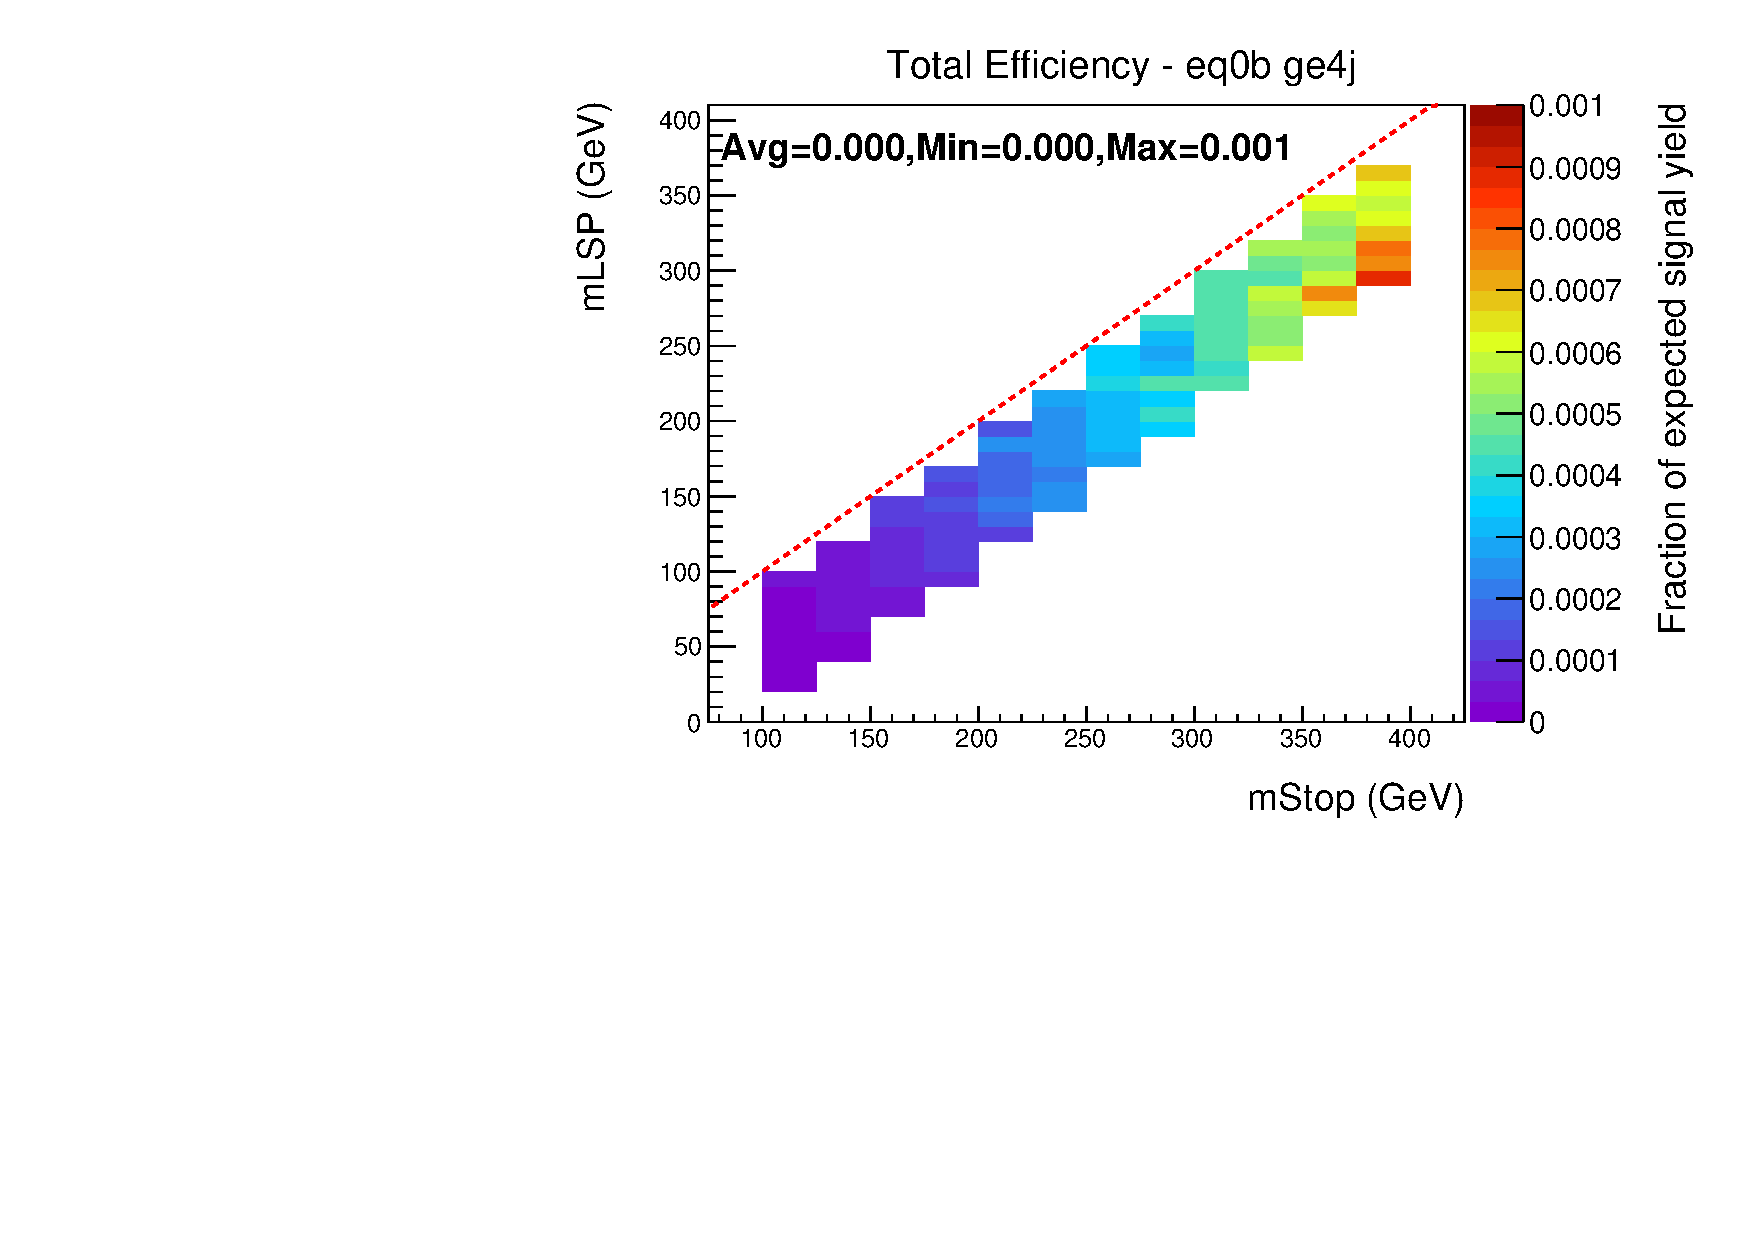
\includegraphics[width=\textwidth, trim=0 0 0 24, clip=true]{Figs/sms/t2degen/v5/T2_4body_v5_had_eff_maps_eq0b_ge4j_SITV.pdf}
    \caption{Signal region, ($\geq 4$,0)}
    \label{fig:t2_4body_sig_eff_ge4j_0b}
  \end{subfigure}
  \begin{subfigure}[b]{0.47\textwidth}
    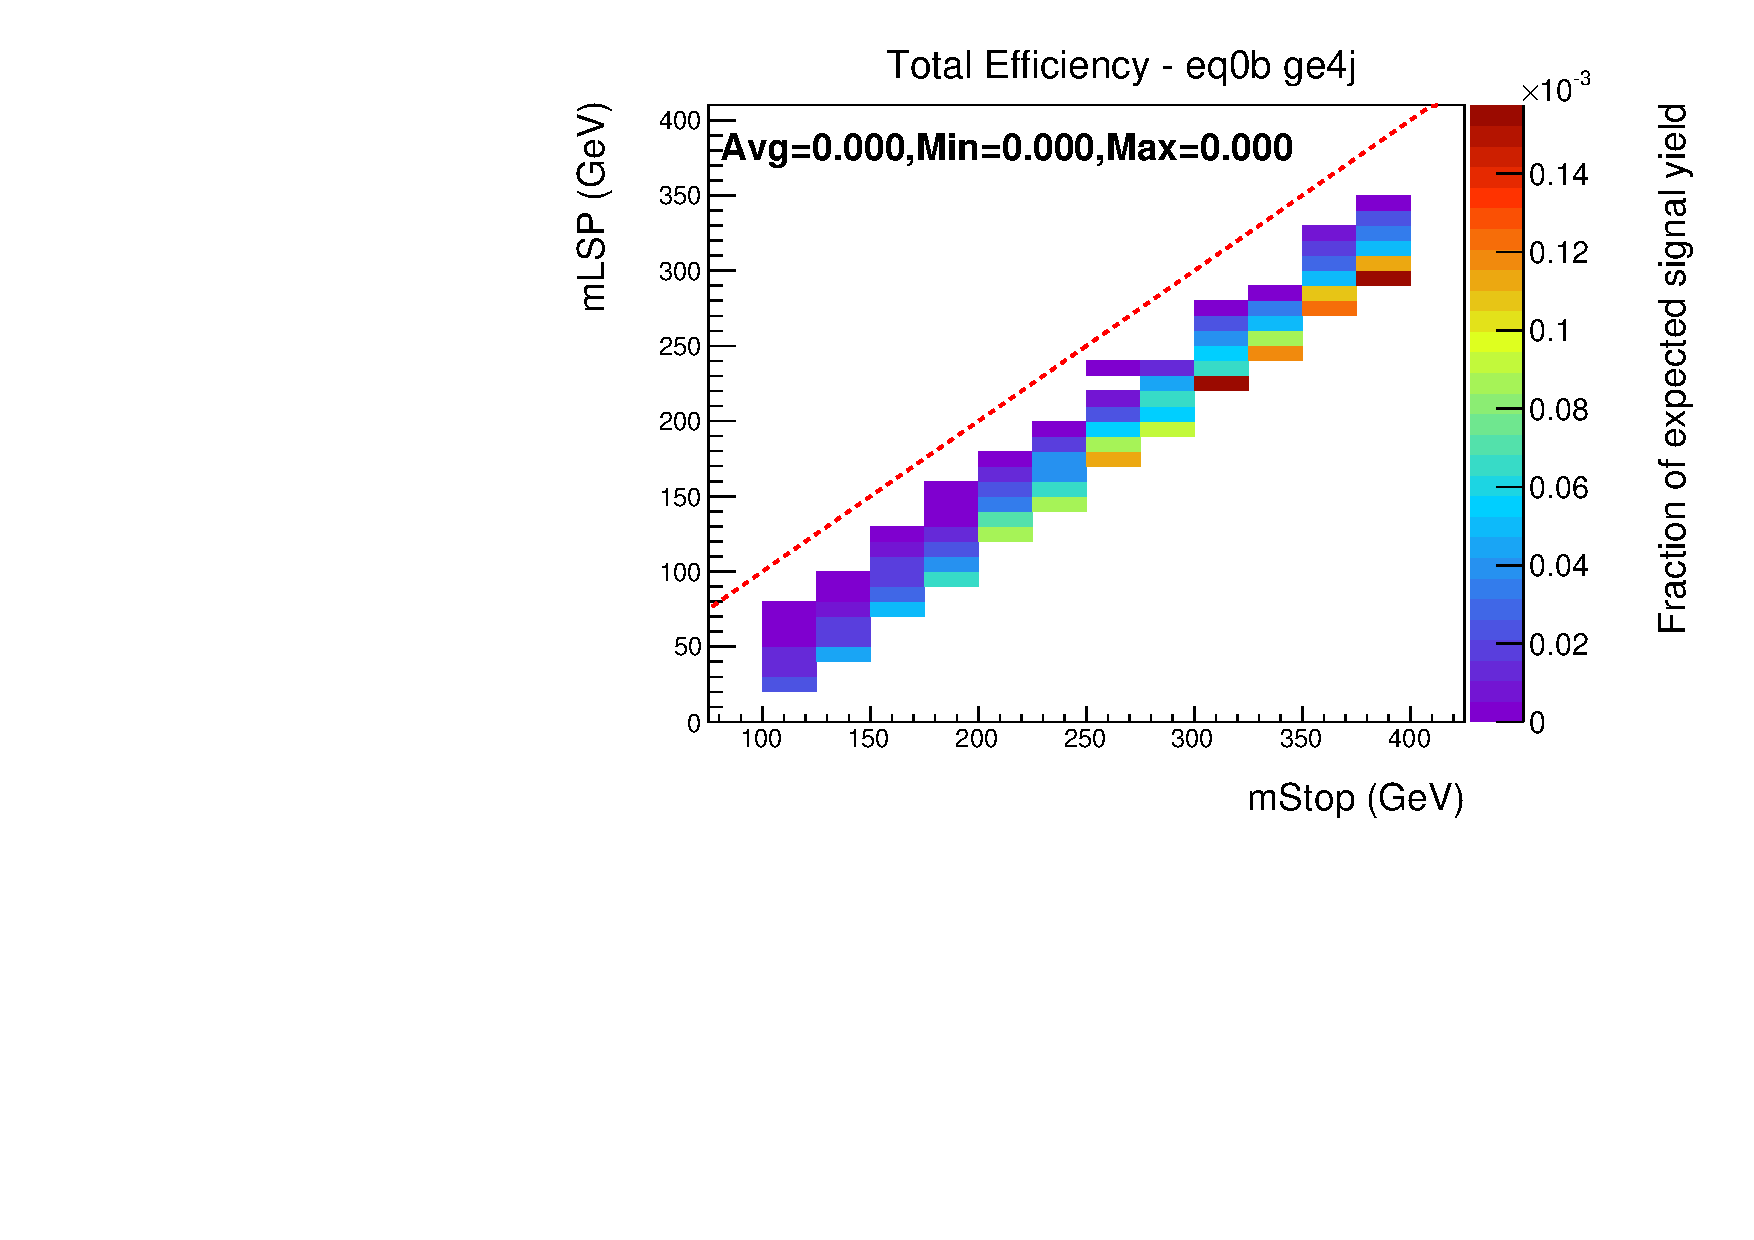
\includegraphics[width=\textwidth, trim=0 0 0 24, clip=true]{Figs/sms/t2degen/v5/T2_4body_v5_muon_eff_maps_eq0b_ge4j_SITV.pdf}
    \caption{\mj region, ($\geq 4$,0)}
    \label{fig:t2_4body_mu_eff_ge4j_0b}
  \end{subfigure} \\
  \begin{subfigure}[b]{0.47\textwidth}
    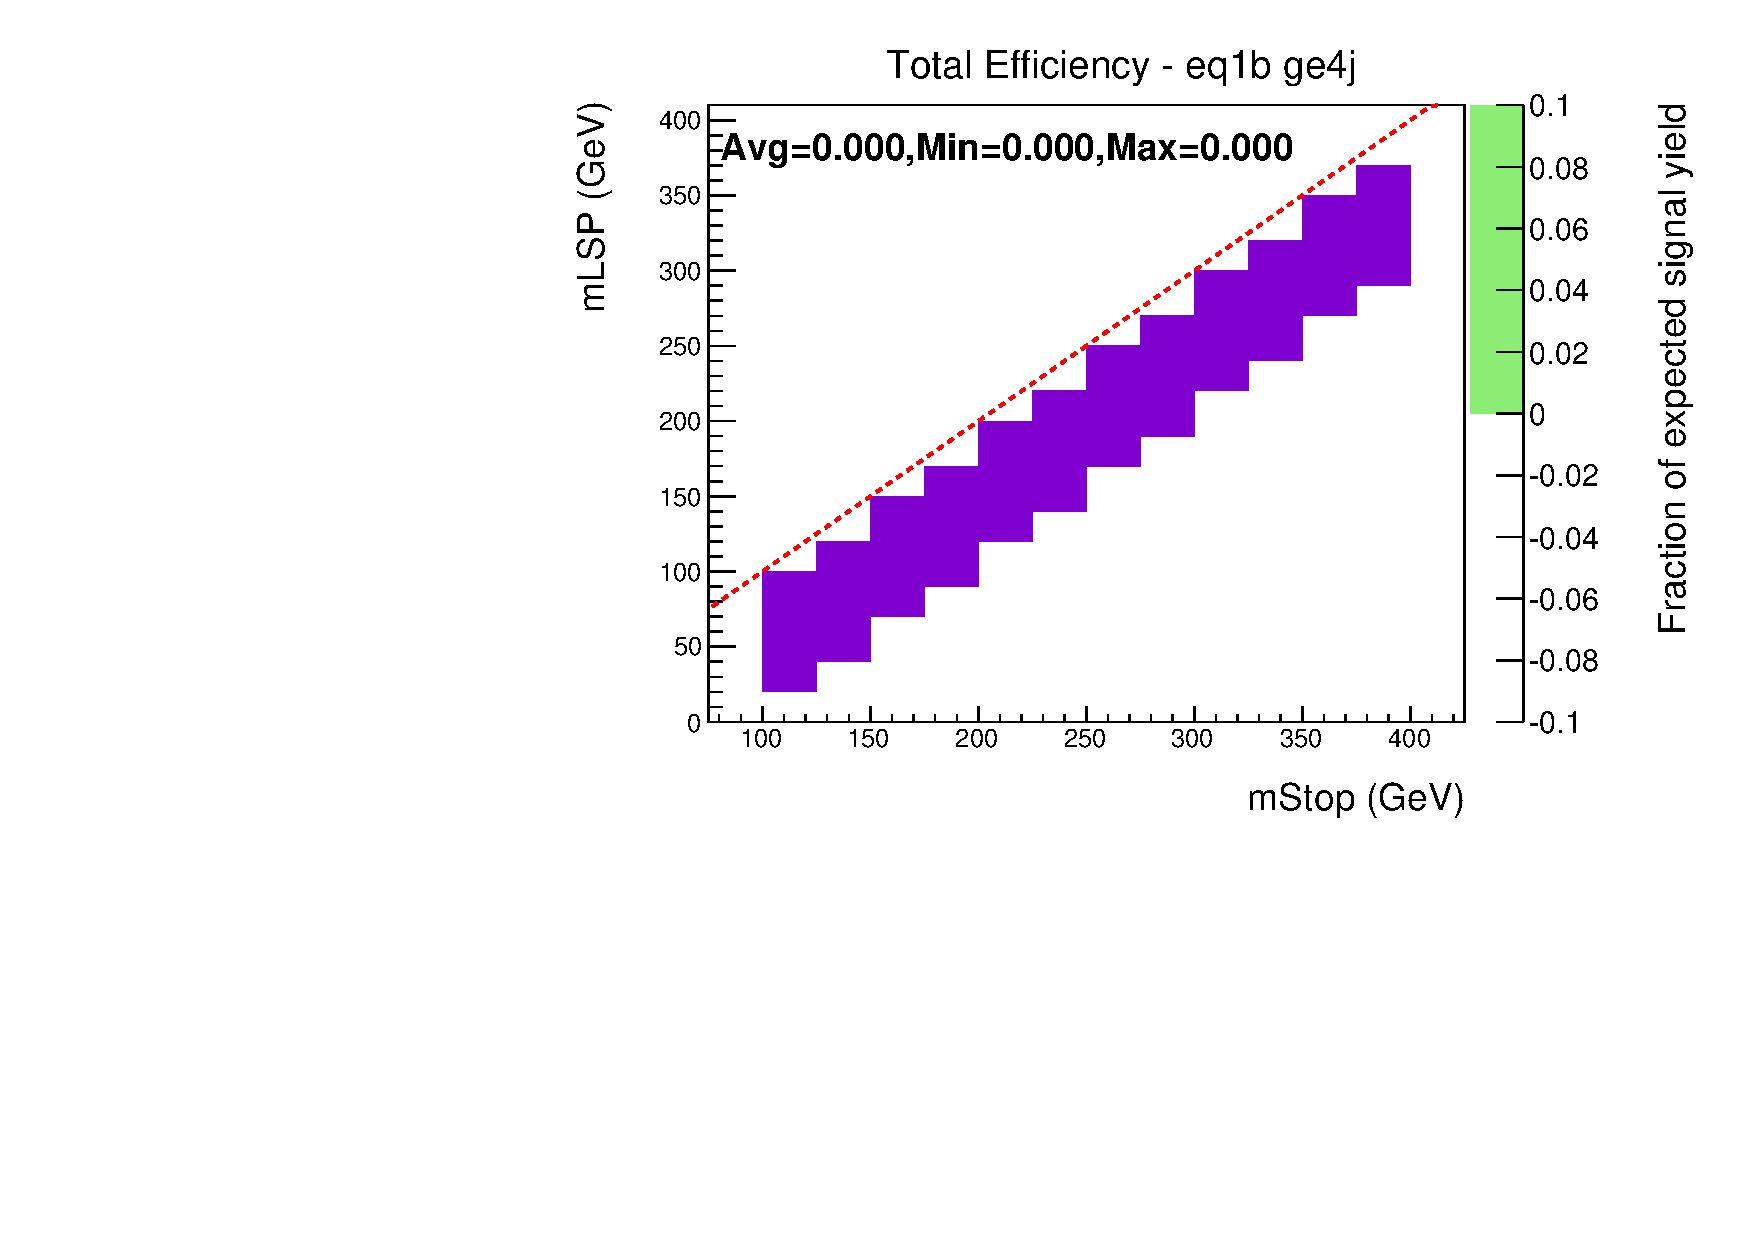
\includegraphics[width=\textwidth, trim=0 0 0 24, clip=true]{Figs/sms/t2degen/v5/T2_4body_v5_had_eff_maps_eq1b_ge4j_SITV.pdf}
    \caption{Signal region, ($\geq 4$,1)}
    \label{fig:t2_4body_sig_eff_ge4j_1b}
  \end{subfigure}
  \begin{subfigure}[b]{0.47\textwidth}
    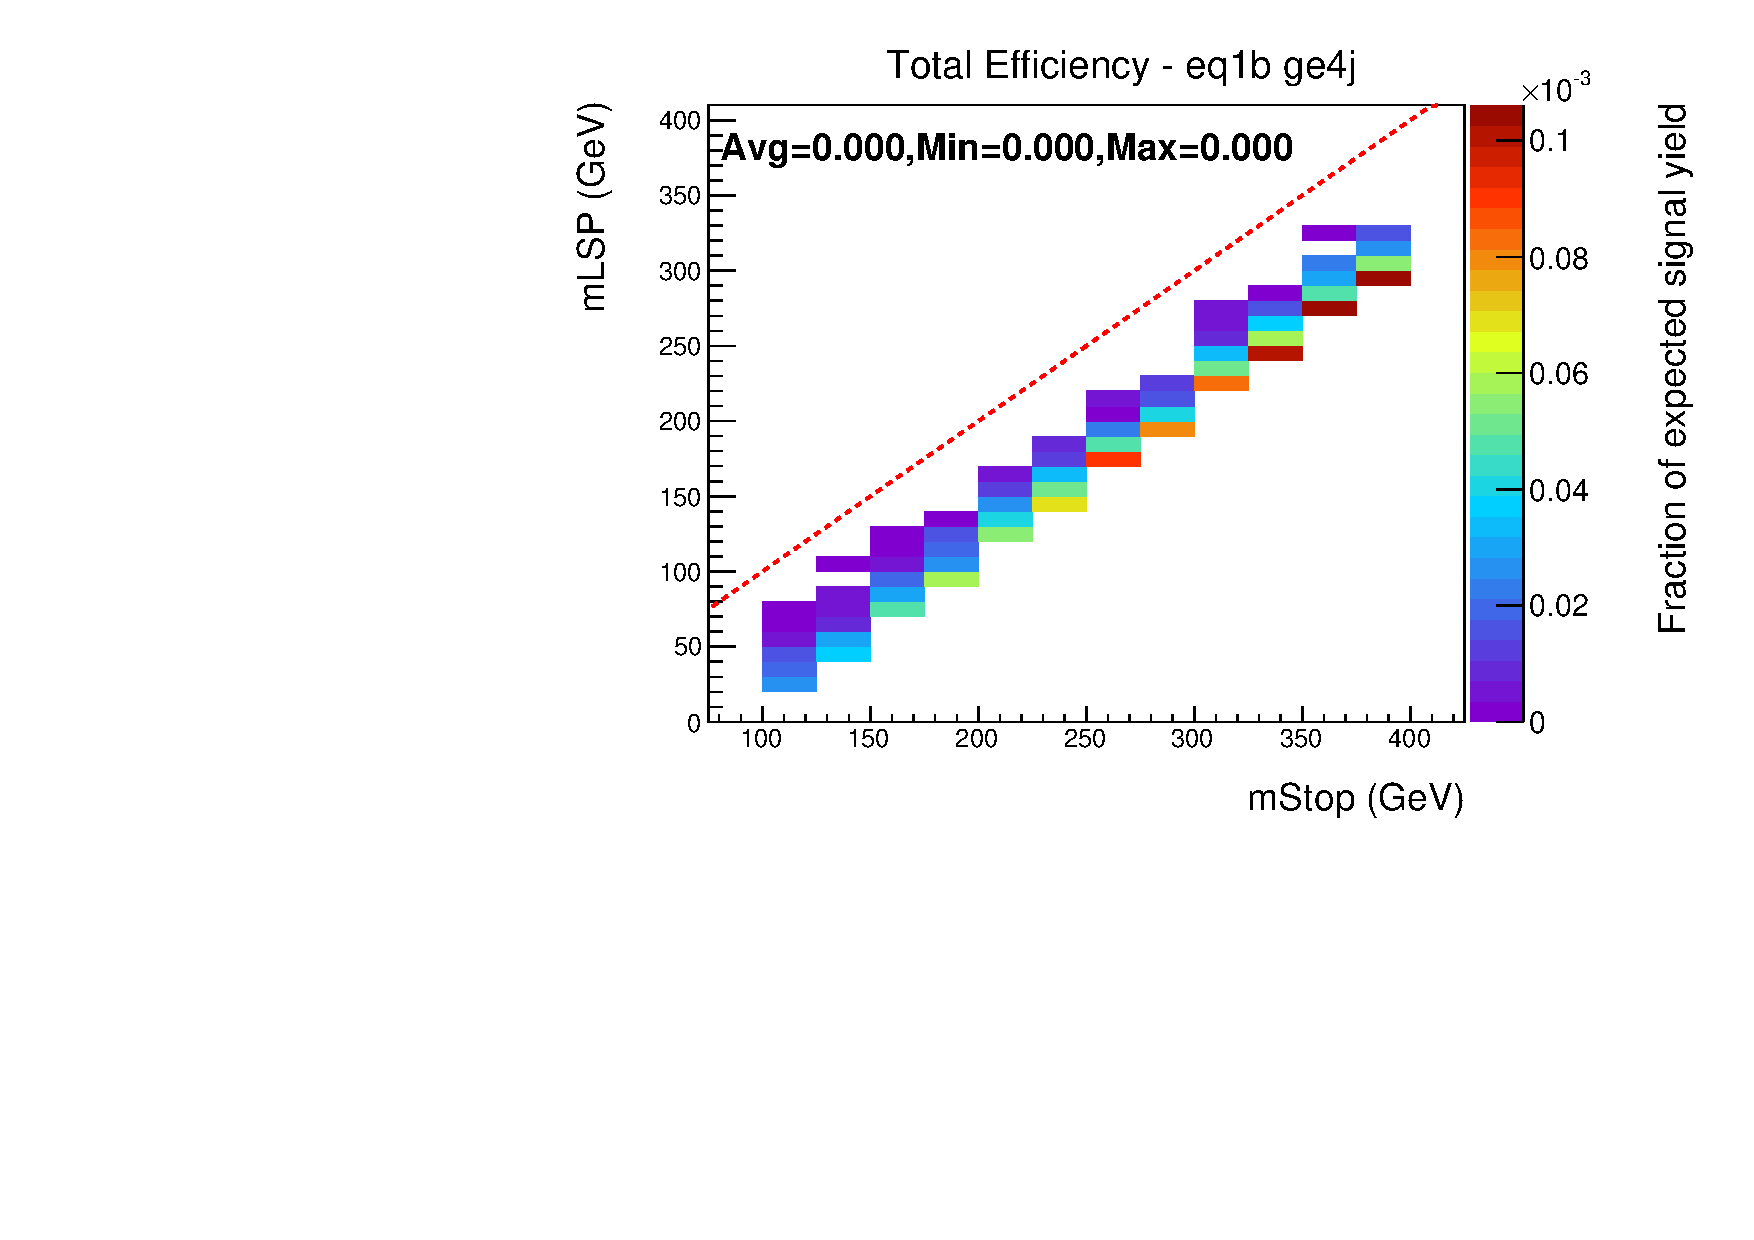
\includegraphics[width=\textwidth, trim=0 0 0 24, clip=true]{Figs/sms/t2degen/v5/T2_4body_v5_muon_eff_maps_eq1b_ge4j_SITV.pdf}
    \caption{\mj region, ($\geq 4$,1)}
    \label{fig:t2_4body_mu_eff_ge4j_1b}
  \end{subfigure} \\
  \caption{Signal efficiency times acceptance for the \Ttwodegen simplified, for 
  the hadronic selection (left) and the \mj selection (right), shown for the 
  four most sensitive analysis categories with an inclusive selection on \HT.}
  \label{fig:t2_4body_eff}
\end{figure}

\subsubsection{Boost corrections to T2\_4body}
Following generator level studies of the \texttt{T2degen} sample a discrepancy 
between the stop system's boot \Pt with respect to the \texttt{T2cc} sample. As 
the kinematics of the stop system should have no dependence whatsoever on the 
decay channel, any discrepancy must be artificial [BETTER WORD?], and should 
therefore be corrected. To determine the magnitude of the required corrections, 
a direct comparison between the two samples was made, as shown in
figure~\ref{fig:t2degen_boost_compare}.

\begin{figure}[h!]
  \centering
    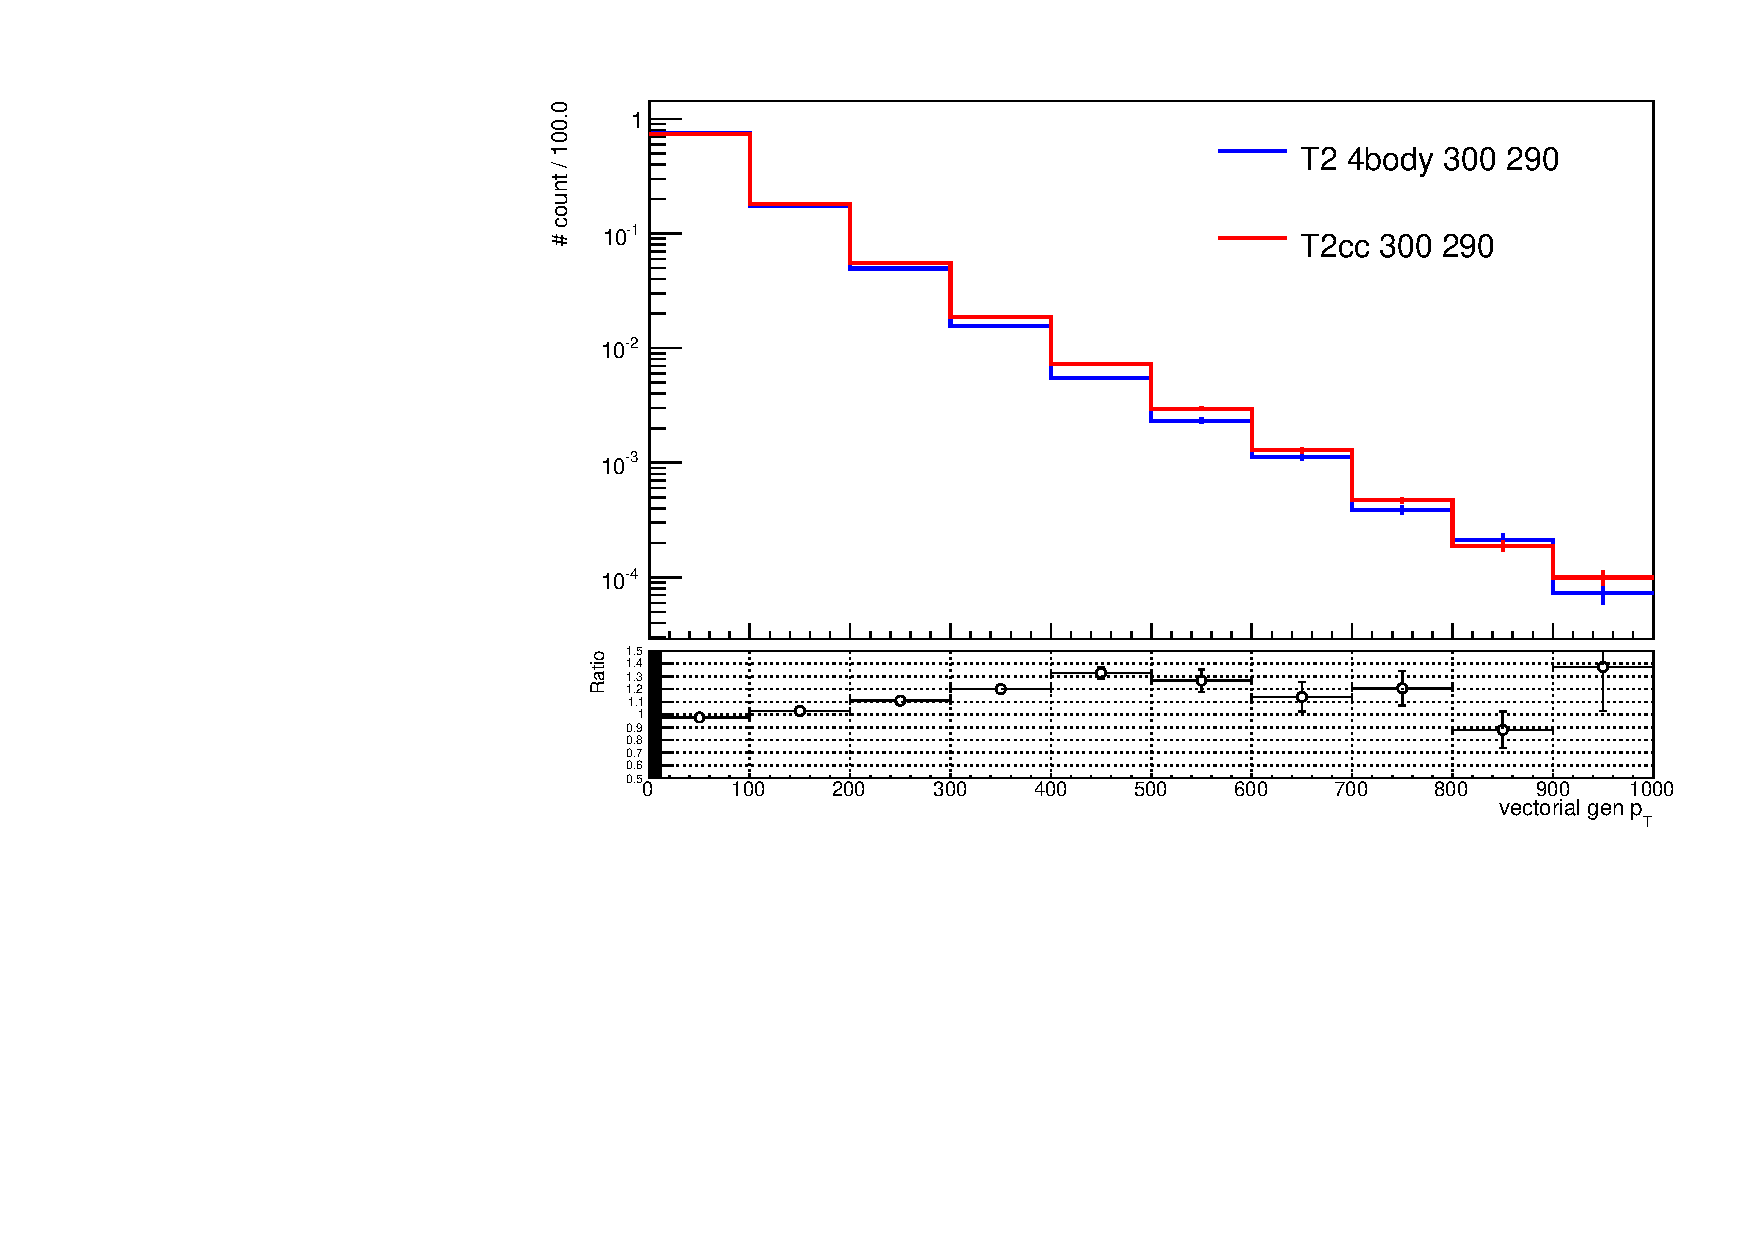
\includegraphics[width=0.6\textwidth]{Figs/sms/t2degen/corrs/compar_stopGenPtVect_0_inc_inc_T2cc_noCuts_sitv_log.pdf}
  \caption{Comparison of the vectorial sum generator-level \Pt of the
  pair-produced \sTop particles, between the \texttt{T2cc} (red) and
  \texttt{T2Degen} (blue) 
  samples, for the mass point (300, 290) \gev. No selection cuts are made and 
  plots are each normalised to a unit area.}
  \label{fig:t2degen_boost_compare}
\end{figure}

Corrections are taken as the ratio between \texttt{T2Degen} and \texttt{T2cc}
as a function of the boost \Pt, for each value of $m_{\sTop}$ in the scan. The 
values of these corrections are shown in figure~\ref{fig:t2degen_boost_weights}.

\begin{figure}[ht!]
  \centering
    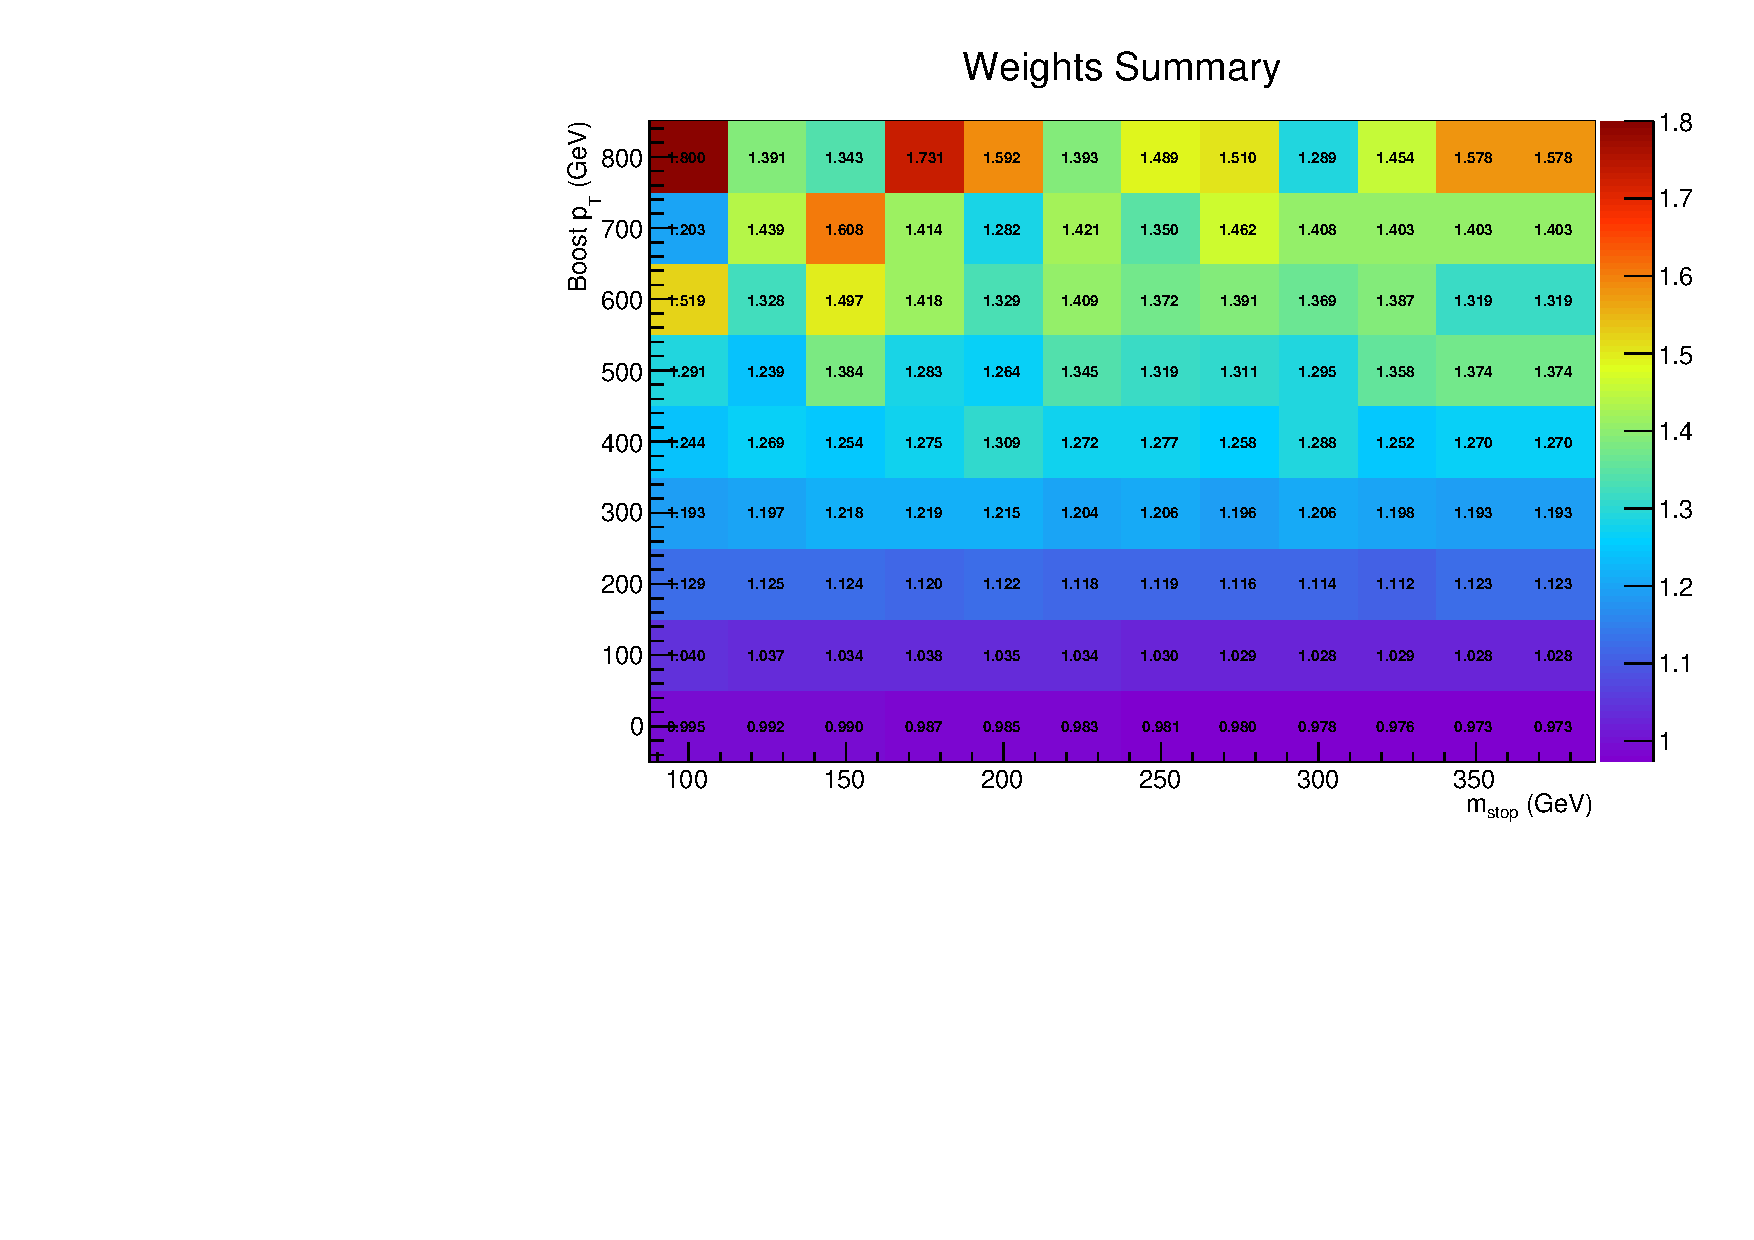
\includegraphics[width=0.8\textwidth]{Figs/sms/t2degen/corrs/stop_lut_weights.pdf}
  \caption{The weights applied to the \texttt{T2degen} sample, shown as a 
  function of $m_{\sTop}$ and boost \Pt.}
  \label{fig:t2degen_boost_weights}
\end{figure}

Acceptance on at the smallest mass-splittings should be in agreement between 
both the \texttt{T2cc} and \texttt{T2Degen} samples following these corrections,
as sensitivity comes entirely from ISR jets and therefore the boost spectrum of 
the \sTop particles. As shown in MAKE PLOT SHOWING AGREEMENT

\subsection{ISR Corrections to compressed spectra MC signal samples}
\label{sec:isr_reweighting}

Given the reliance of such compressed spectra models on ISR jets for acceptance,
a dedicated study was performed within the SUSY PAG into it's accuracy and 
relevant systematic uncertainties [REF].

A comparison of data to MC was performed for a high-statistics, pure selection of Z boson 
production with associated jets, where the Z decays to an opposite-sign,
same-flavour (OSSF) lepton pair, $Z\ra l\bar{l}$. By tagging the leptons in 
the event, any other jets can be considered as an ISR jet based ``recoil system'' 
against that of the Z boson decay. Comparisons of data to MC for both the 
vectorial sum of the lepton \Ptvect's and the recoil jet \Ptvect's indicate an
over-prediction in MC as a function of the recoil system's \Pt, of up to 20\% in 
high \Pt scenarios, shown in figure~\ref{fig:isr_datamc}.

Correction factors, dependent on the \Pt of the jet system, for \MADGRAPH based
samples can therefore be derived by extracting the ratio of data to MC. These 
values are summarised in table~\ref{tab:isr_weights}. Weights are applied to 
both \texttt{T2cc} and \texttt{T2degen} samples at the event level, where the 
event's boost \Pt is determined by calculating the vectorial sum of the 
two, pair-produced generator level \sTop particles.

\begin{table}[ht!]
  \caption{Correction factors for \MADGRAPH based signal samples to account for 
  MC over-prediction of ISR.\label{tab:isr_weights}}
  \centering
  \small
  \begin{tabular}{ lc }
    \hline
    \hline
    $\Pt_{boost} (\gev)$    & Correction Factor \\
    \hline
    $0 <\Pt\leq120    $          & 1.00 \\
    $120 <\Pt\leq150  $          & 0.95 \\
    $150 <\Pt\leq250  $          & 0.90 \\
    $250 < \Pt        $          & 0.80 \\    
    \hline
    \hline
  \end{tabular}
\end{table}

\begin{figure}[h]
  \begin{center}
    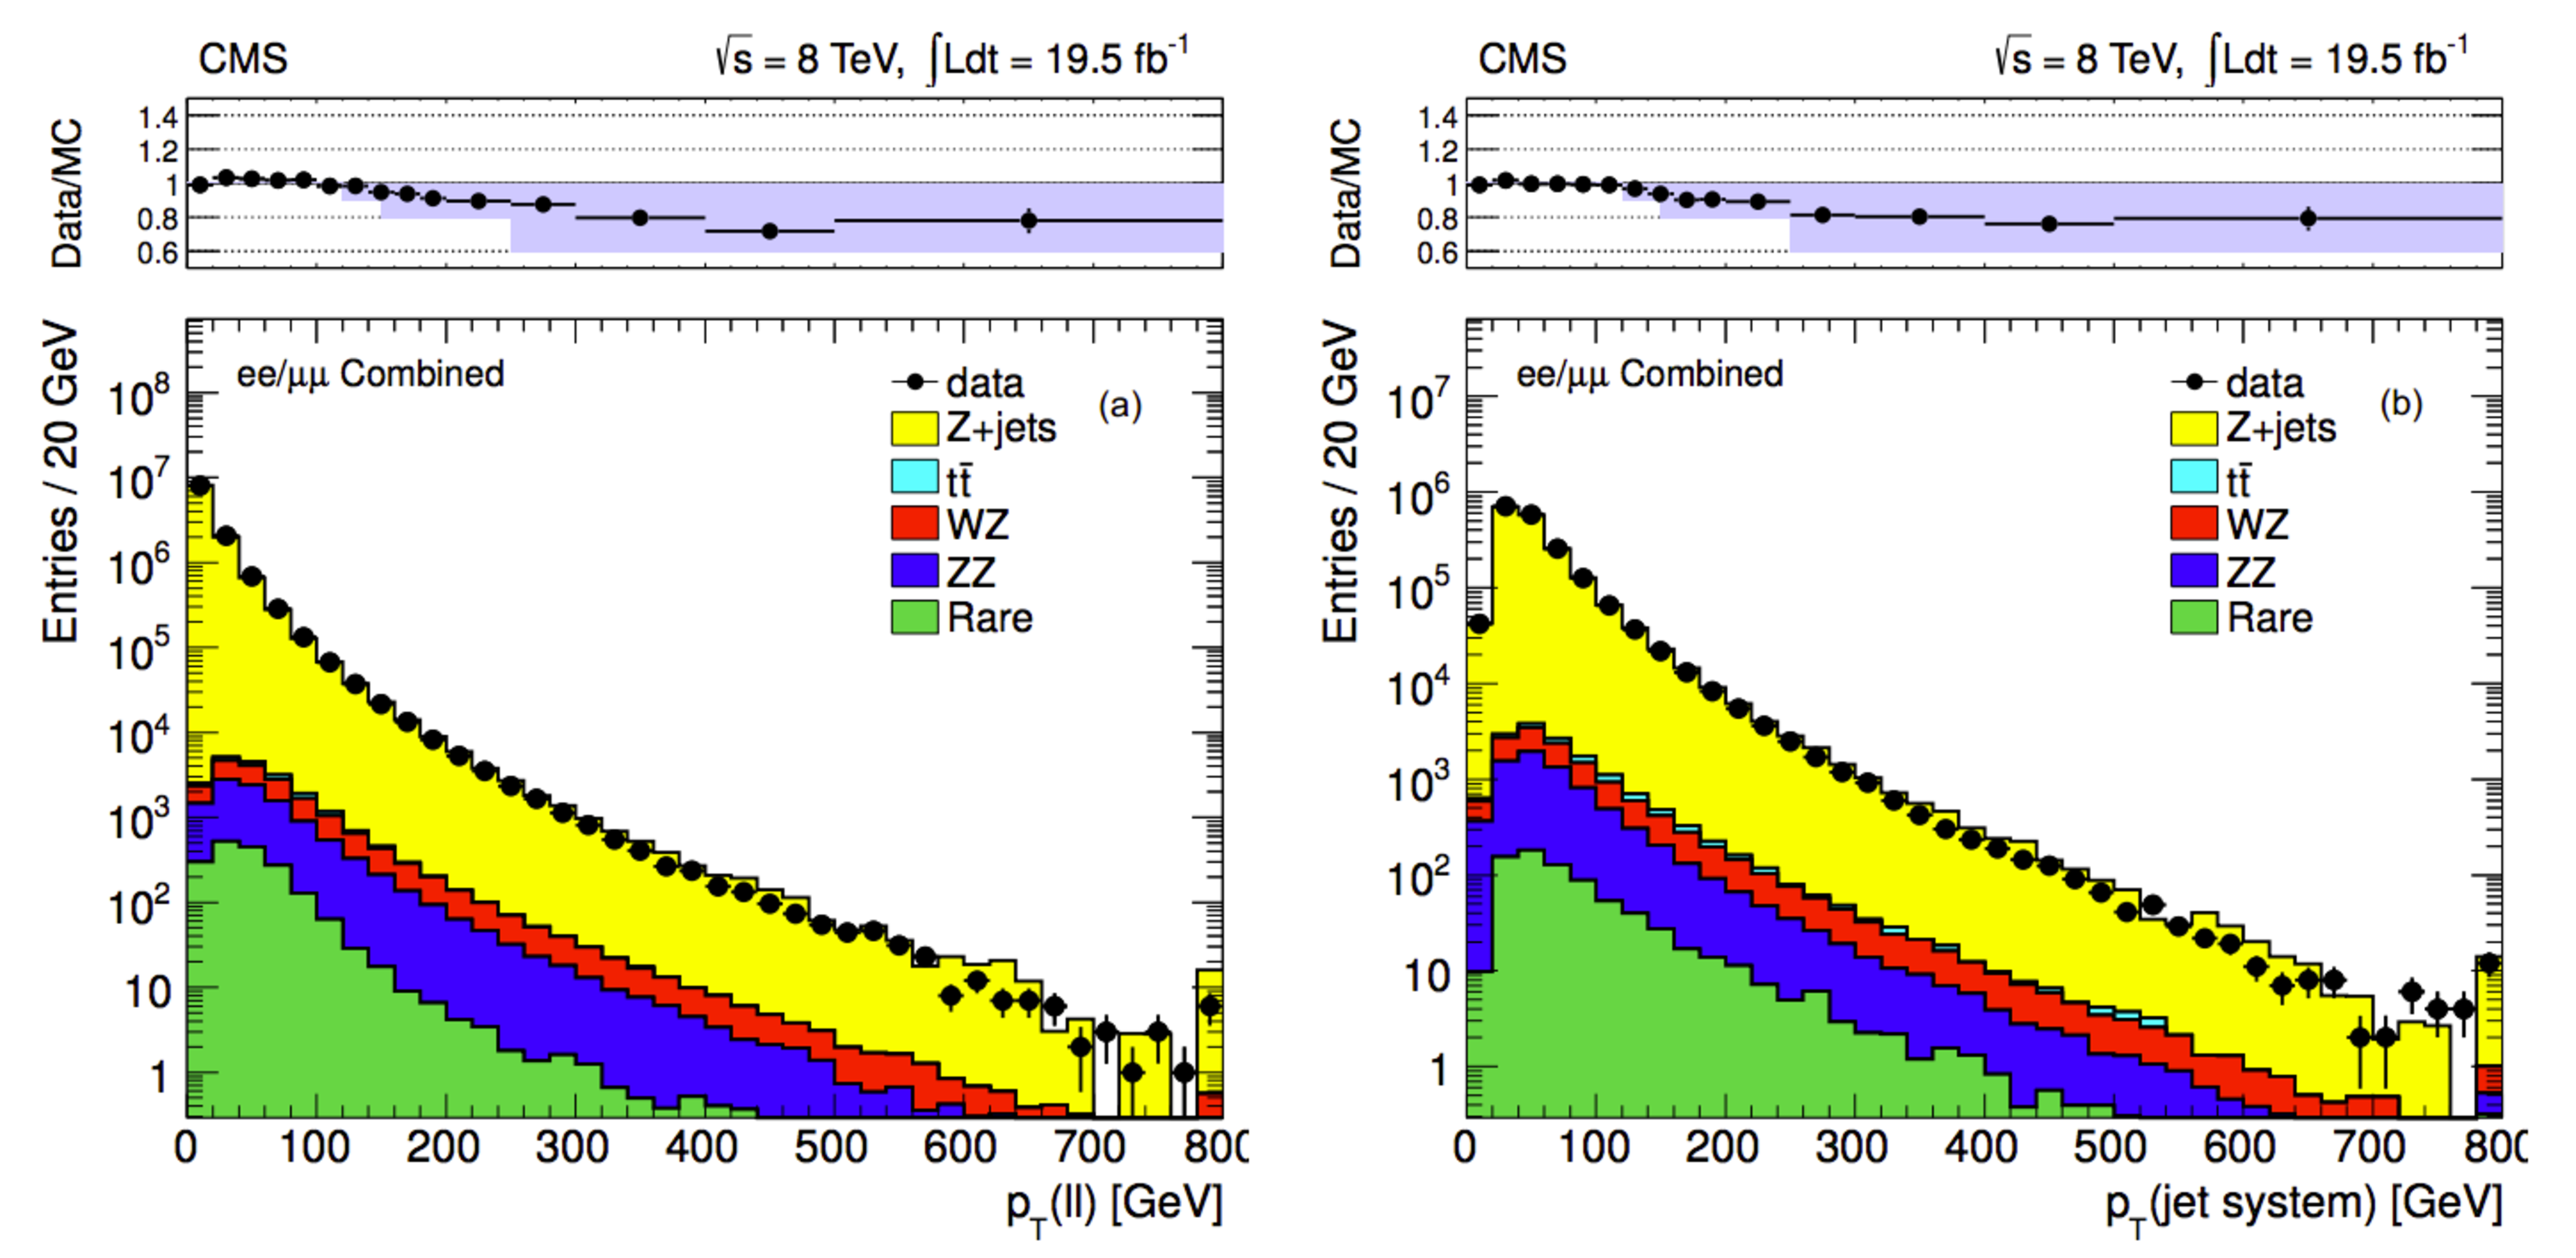
\includegraphics[width=0.8\textwidth]{Figs/isr/isr_zjets_distros.pdf}
    % \caption{blah}
    \caption{Data to MC comparisons for an enriched $Z \ra l\bar{l}$ selection, 
    with the vectorial sum of lepton \Pt's (left) and of the recoil jets (right).
    REF TO PAPER}
    \label{fig:isr_datamc}
  \end{center}
\end{figure}

\emph{show the effect on signal acceptance for T2cc?}

% \begin{figure}[!h]
%  \begin{center}
%    \subfigure[Signal region, (2--3,0)]{
%      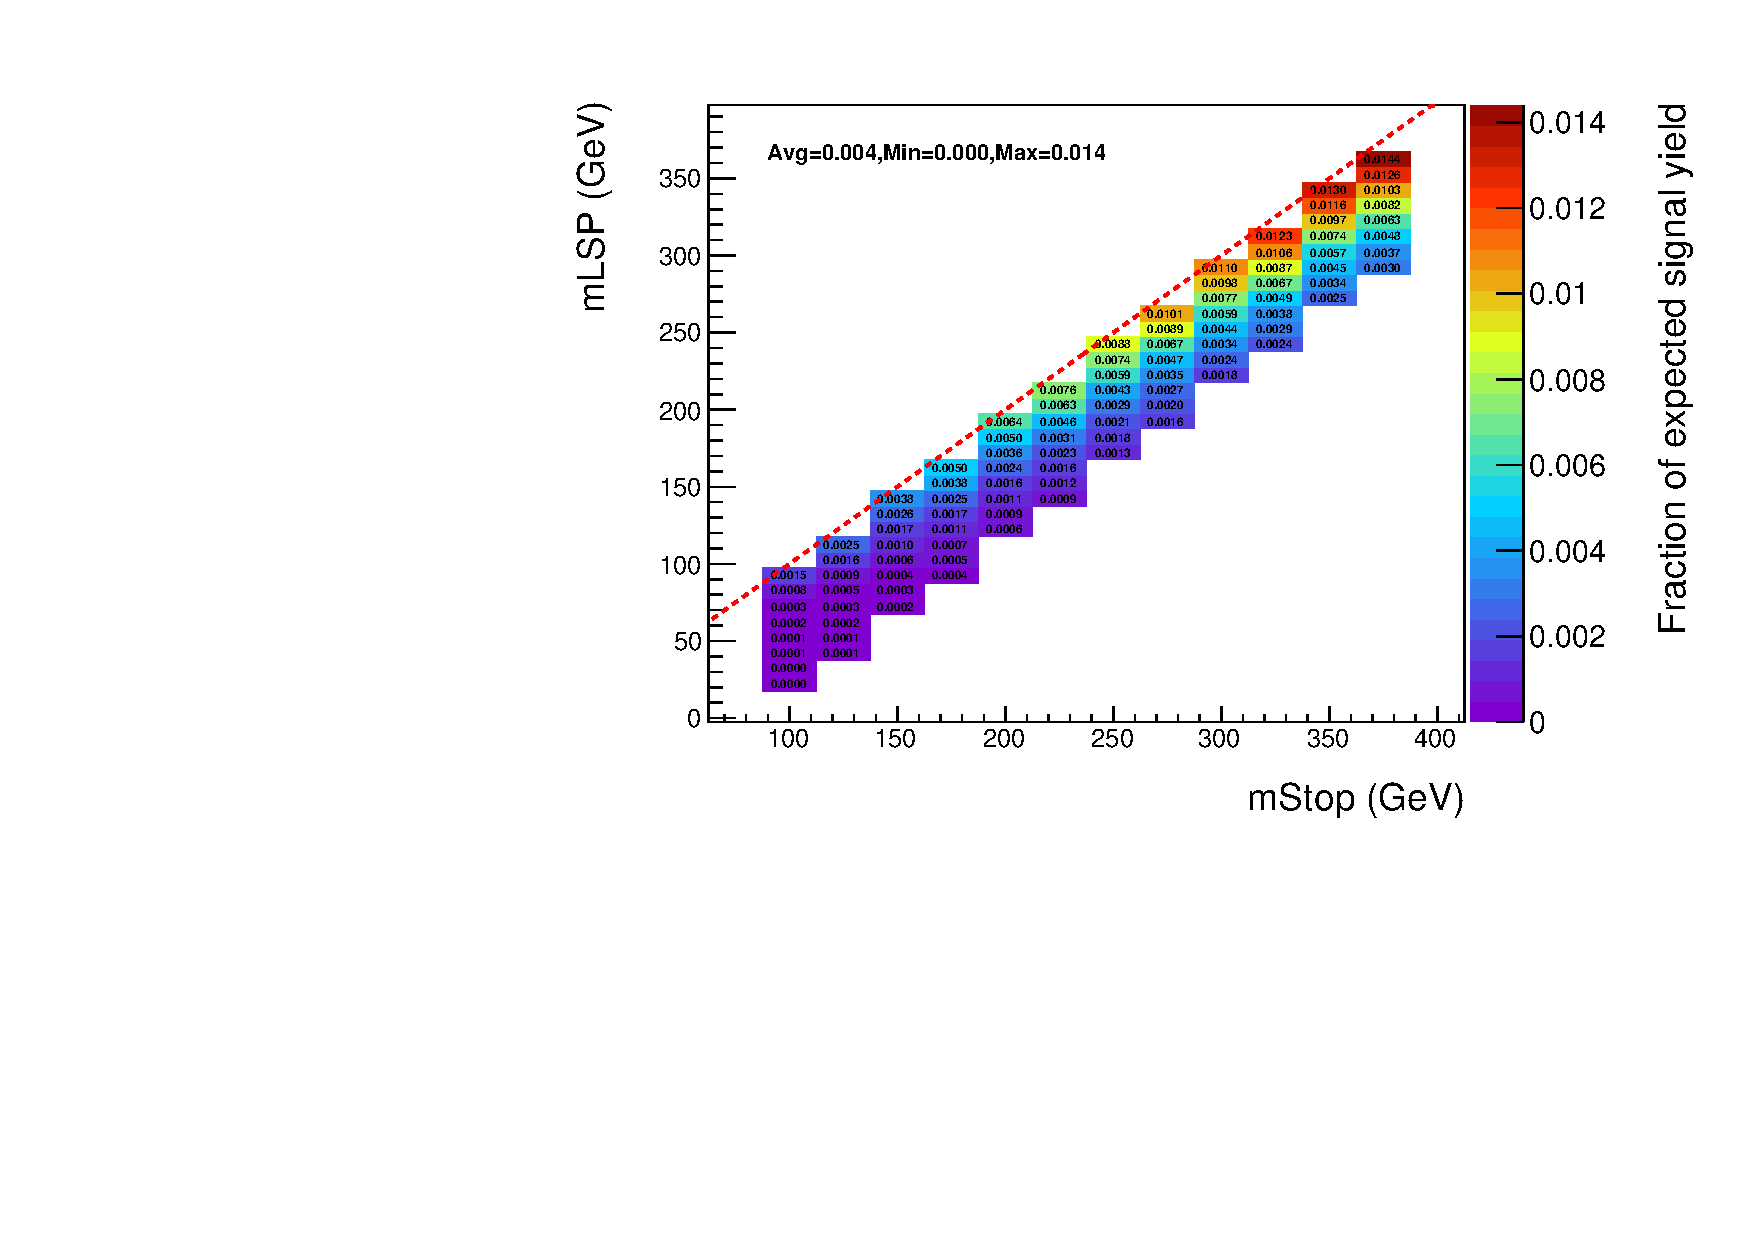
\includegraphics[width=0.4\textwidth]{figures/sms/t2_4body/v16/T2_4body_had_eff_maps_eq0b_le3j_SITV}
%    } 
%    \subfigure[\mj sample, (2--3,0)]{
%      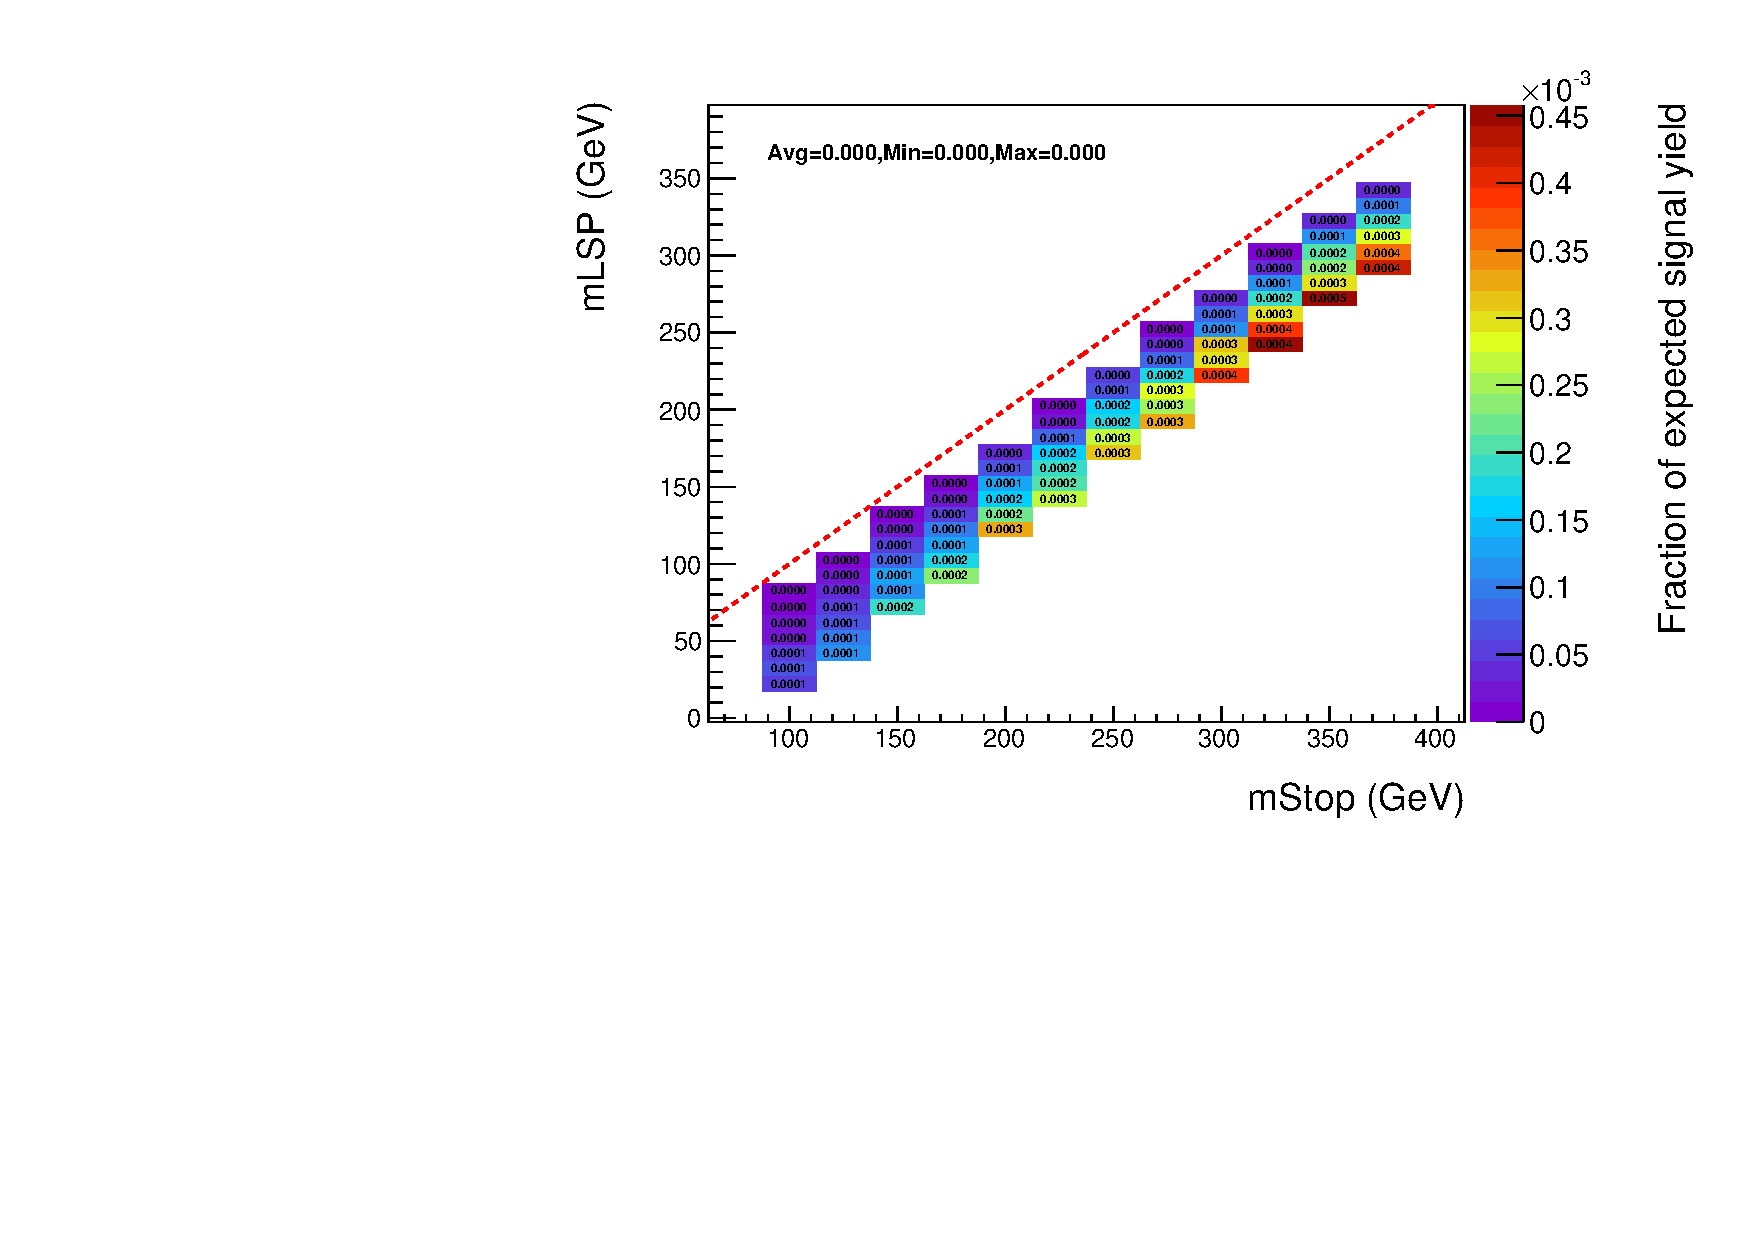
\includegraphics[width=0.4\textwidth]{figures/sms/t2_4body/v16/T2_4body_muon_eff_maps_eq0b_le3j_SITV}
%    } \\
%    \subfigure[Signal region, (2--3,1)]{
%      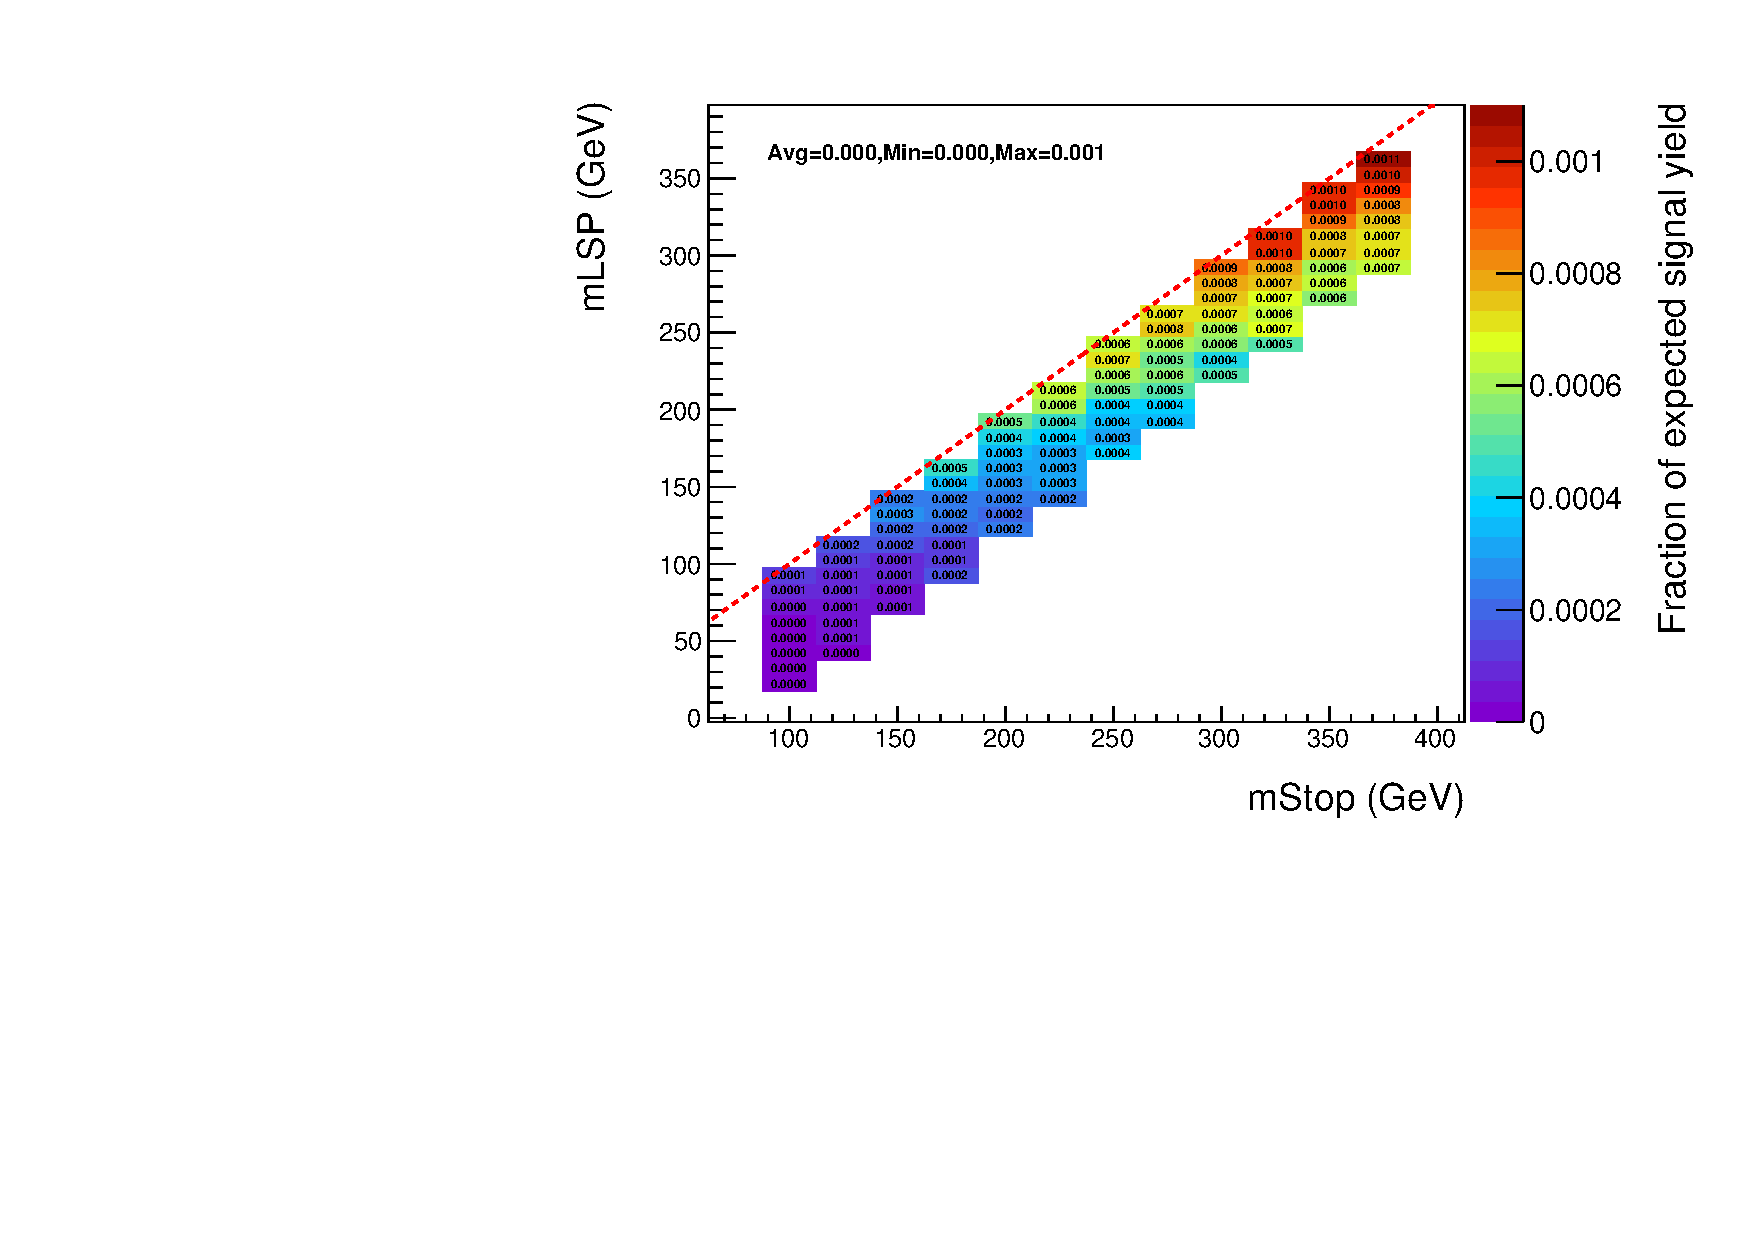
\includegraphics[width=0.4\textwidth]{figures/sms/t2_4body/v16/T2_4body_had_eff_maps_eq1b_le3j_SITV}
%    } 
%    \subfigure[\mj sample, (2--3,1)]{
%      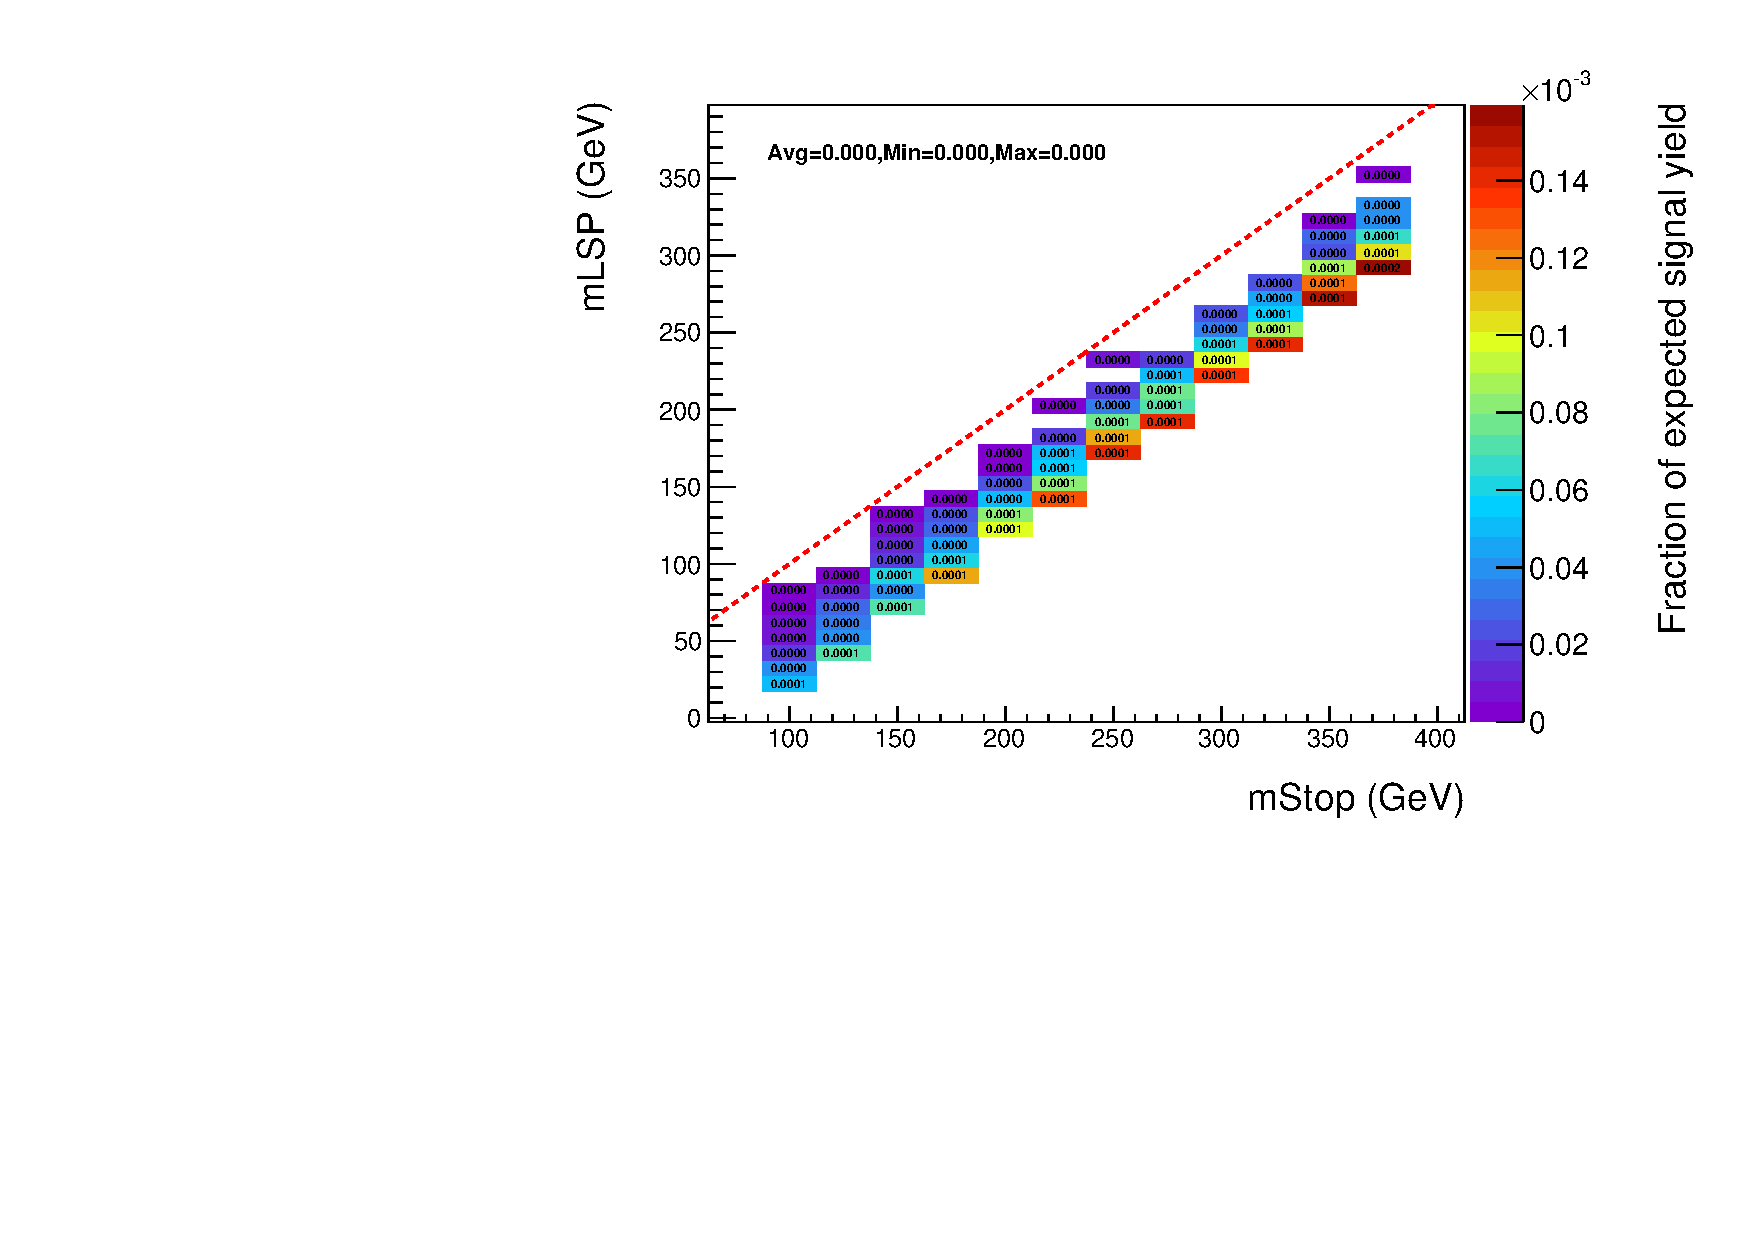
\includegraphics[width=0.4\textwidth]{figures/sms/t2_4body/v16/T2_4body_muon_eff_maps_eq1b_le3j_SITV}
%    } \\
%    \subfigure[Signal region, ($\geq 4$,0)]{
%      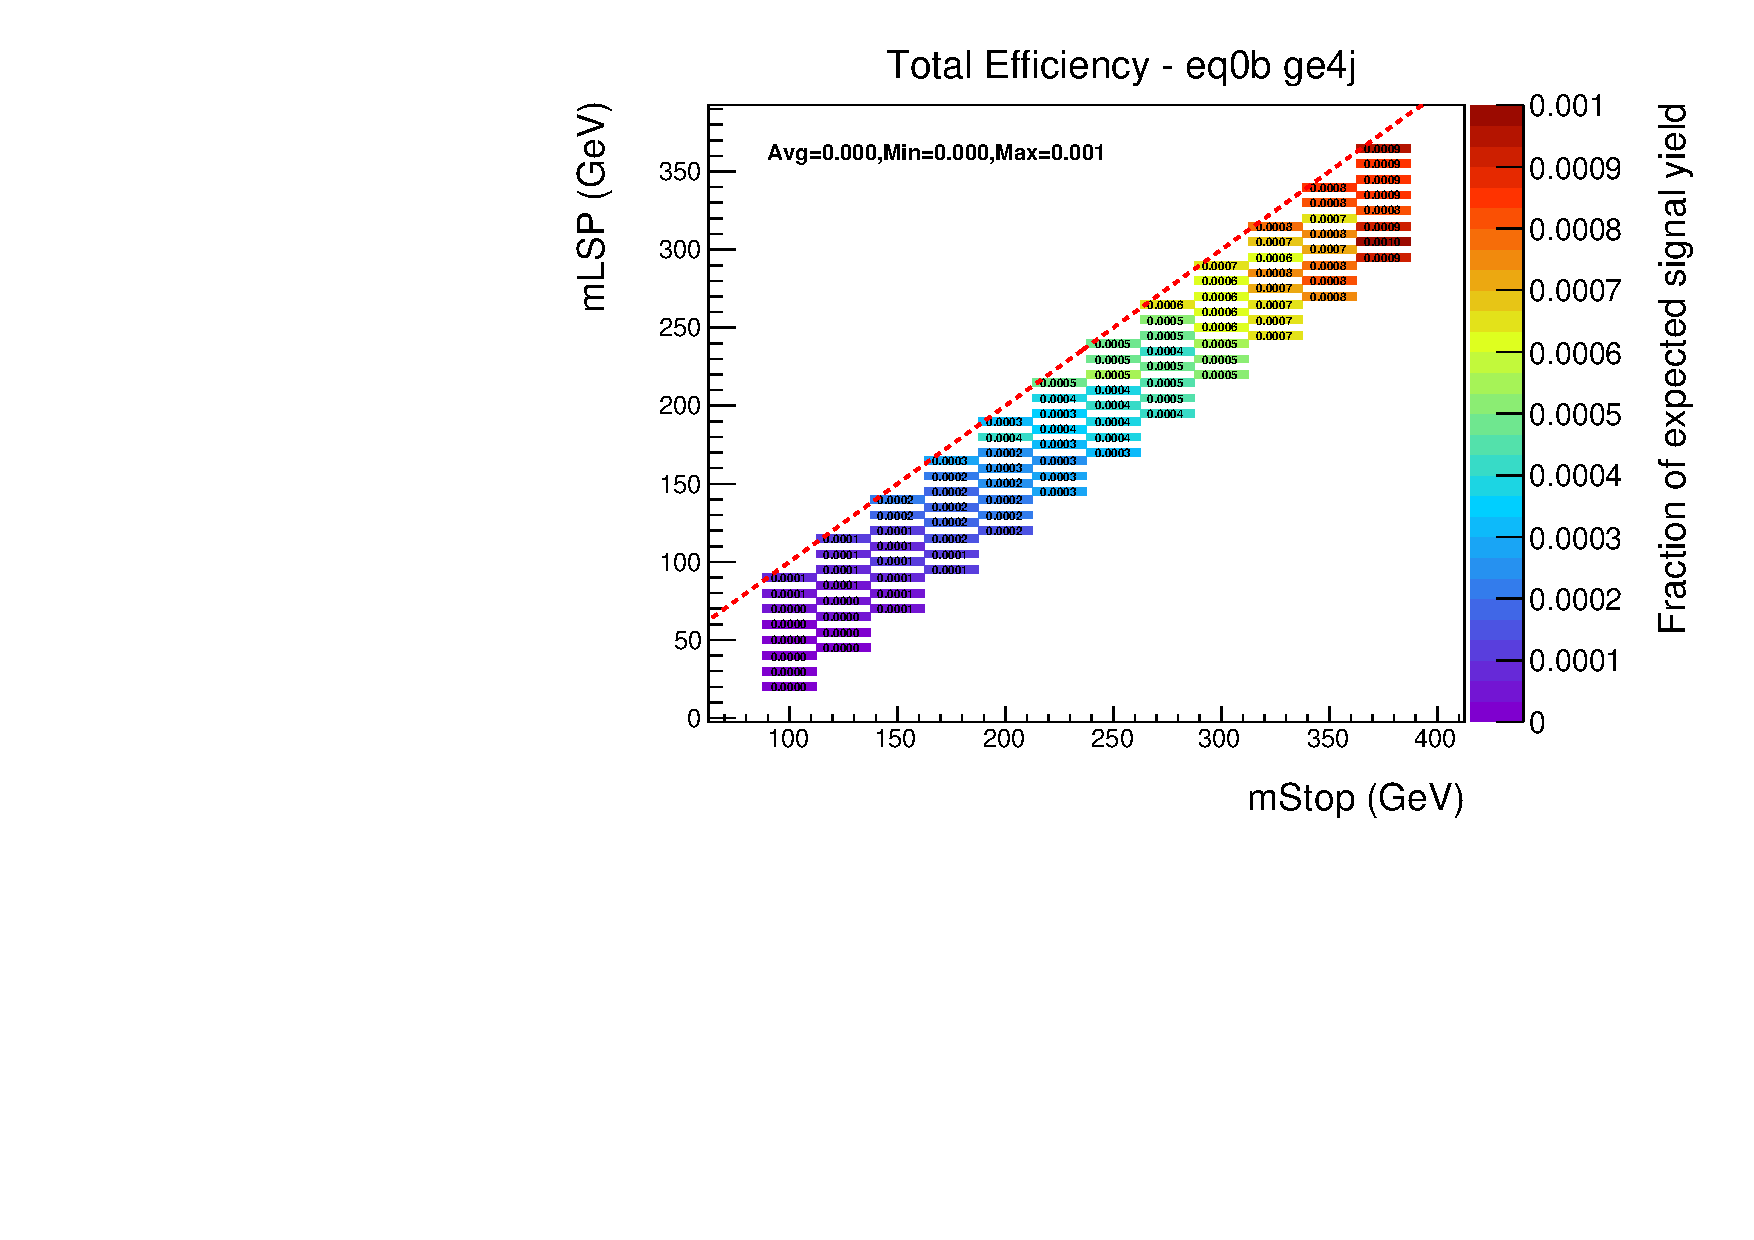
\includegraphics[width=0.4\textwidth]{figures/sms/t2_4body/v16/T2_4body_had_eff_maps_eq0b_ge4j_SITV}
%    } 
%    \subfigure[\mj sample, ($\geq 4$,0)]{
%      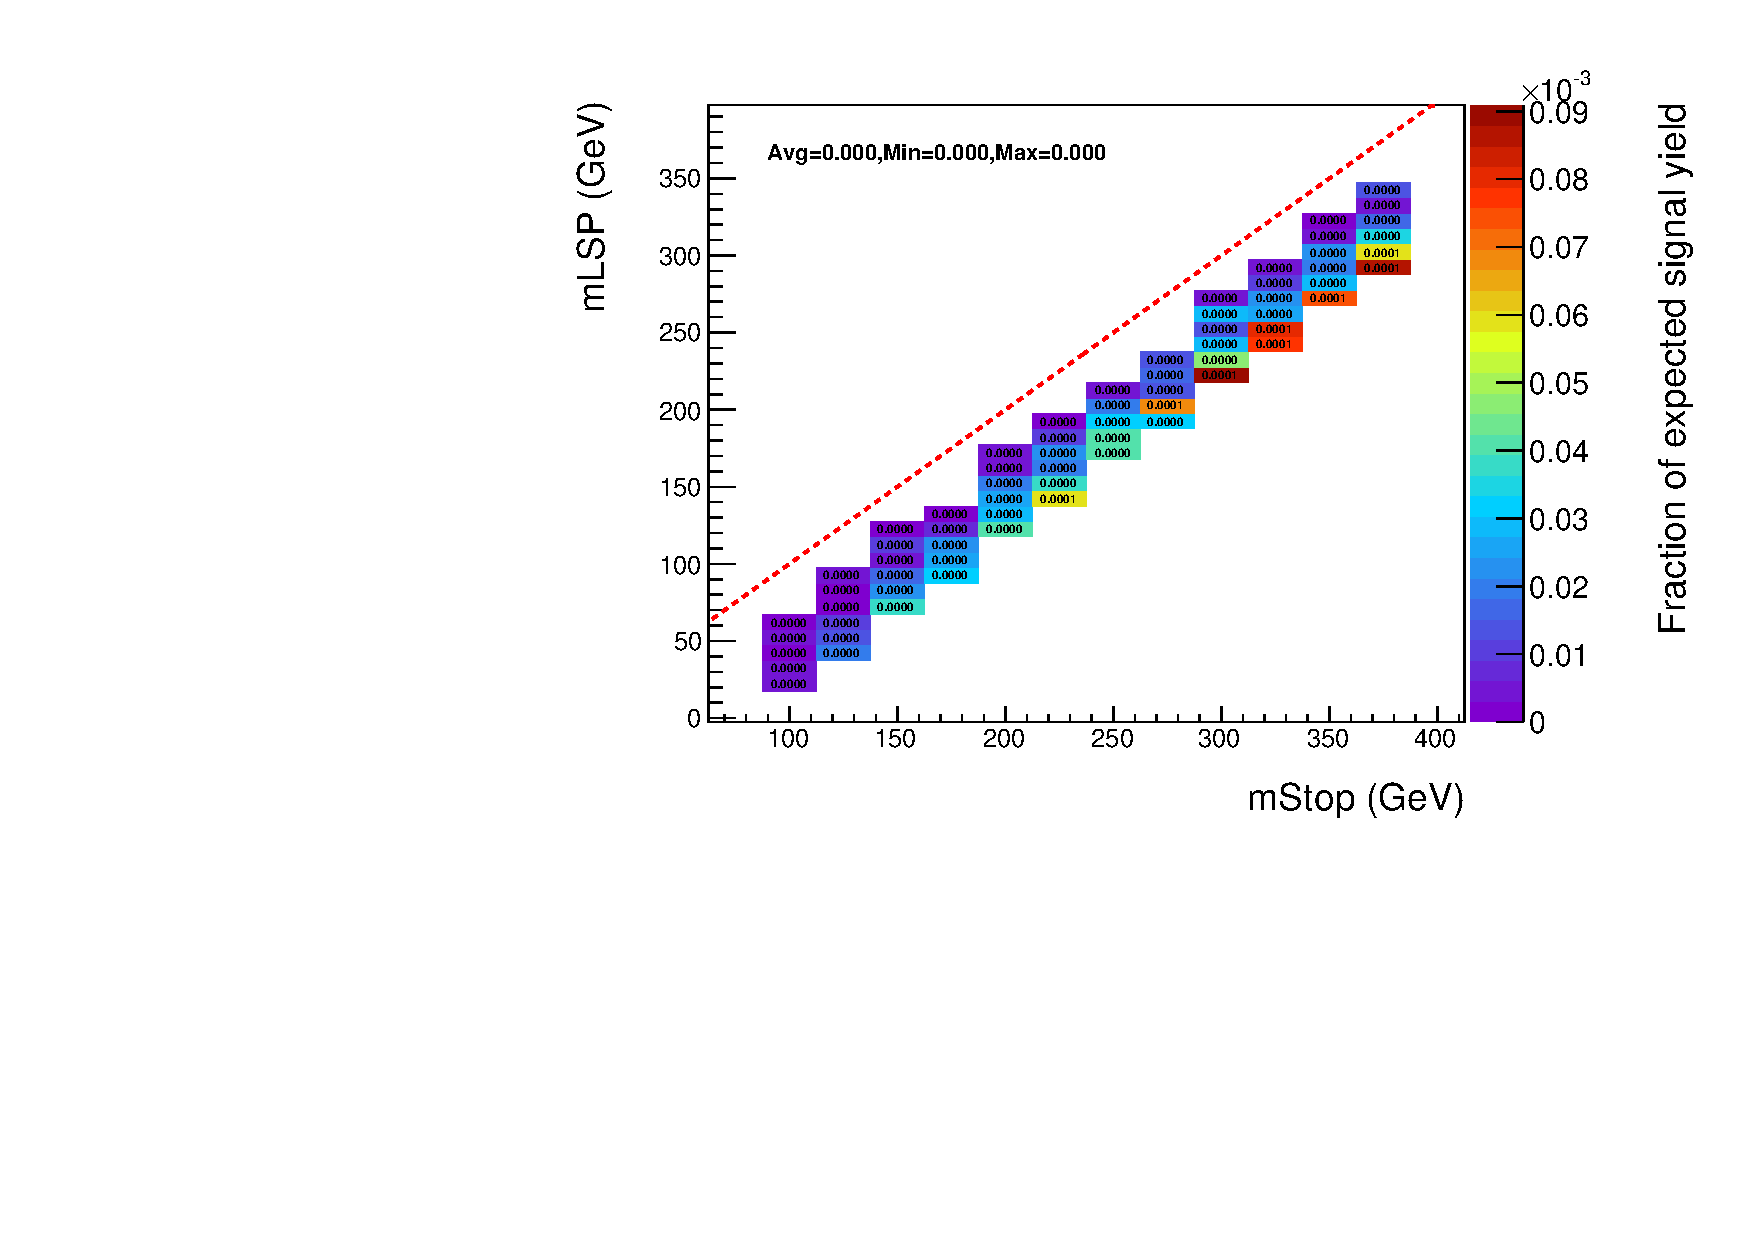
\includegraphics[width=0.4\textwidth]{figures/sms/t2_4body/v16/T2_4body_muon_eff_maps_eq0b_ge4j_SITV}
%    } \\
%    \subfigure[Signal region, ($\geq 4$,1)]{
%      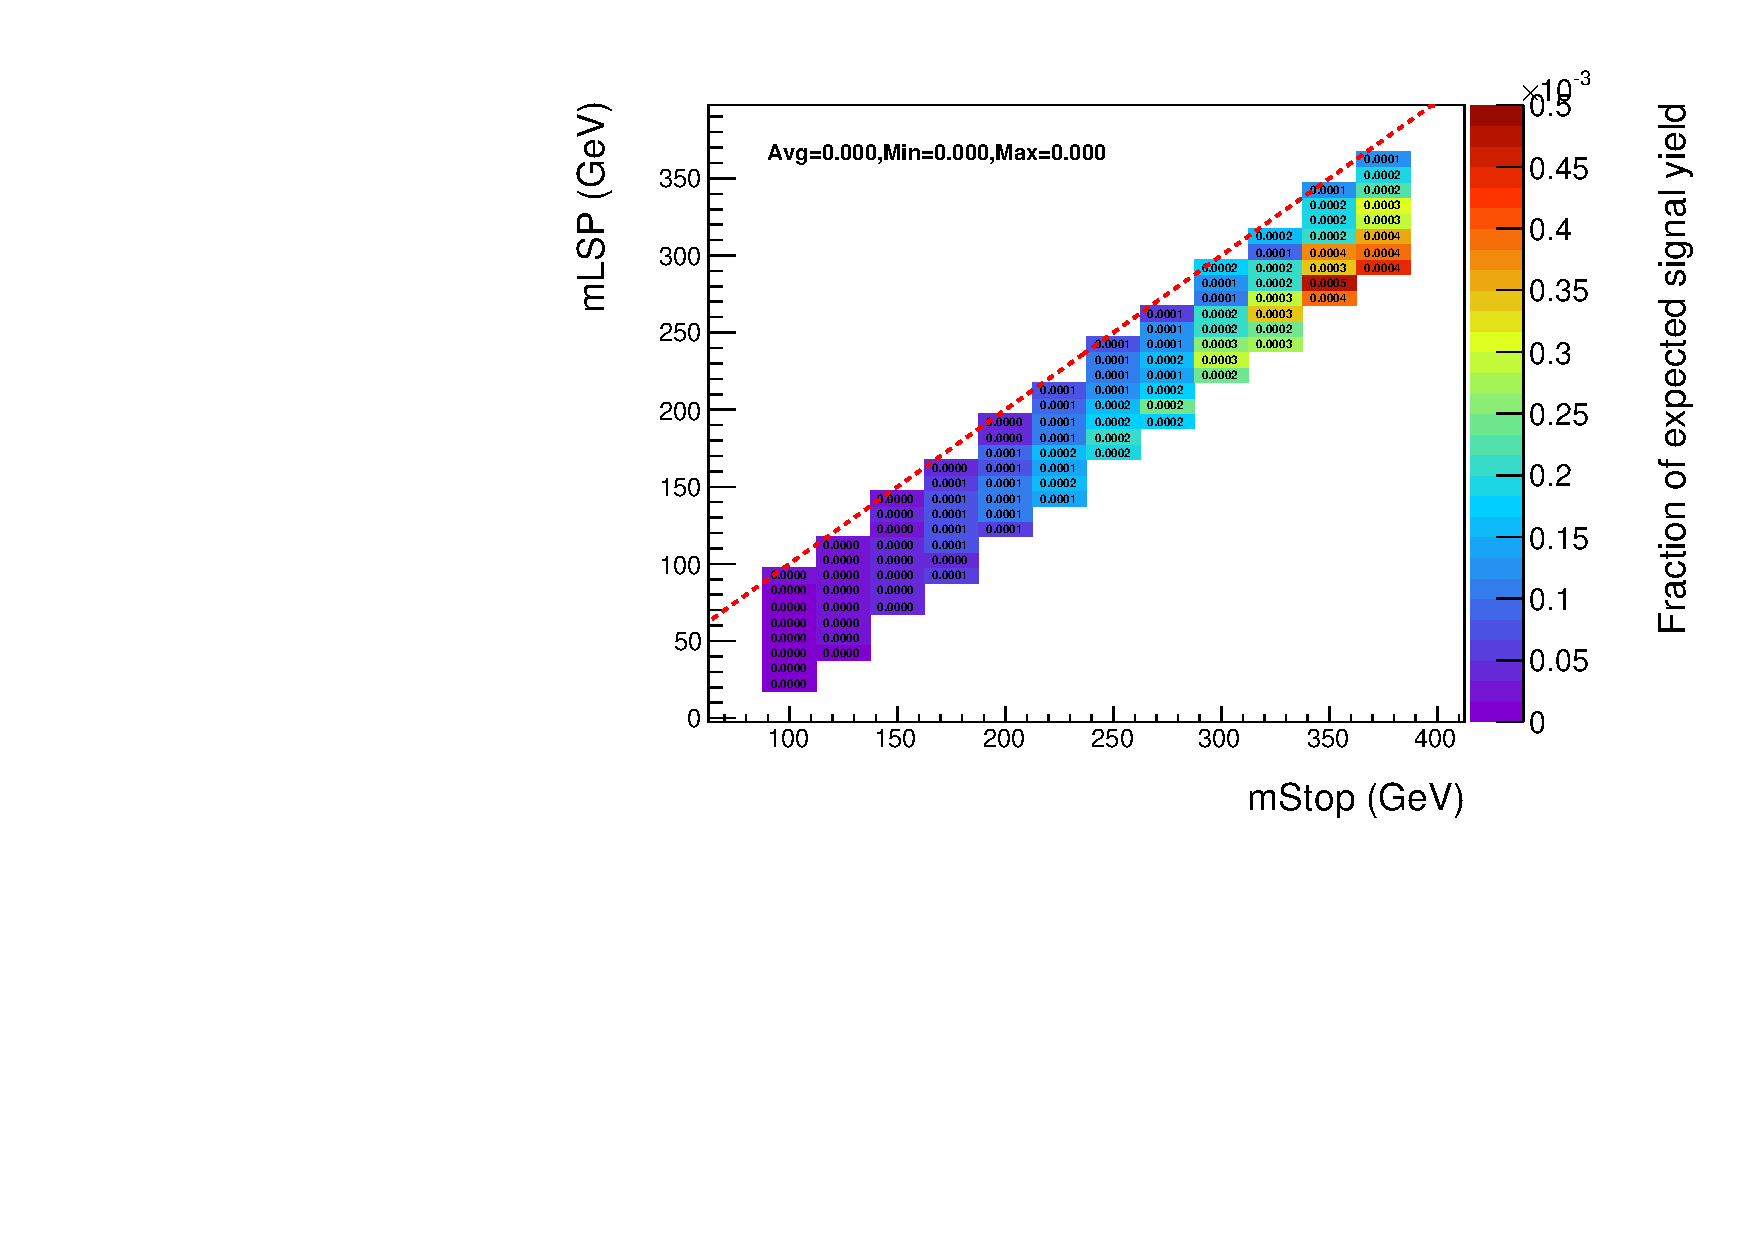
\includegraphics[width=0.4\textwidth]{figures/sms/t2_4body/v16/T2_4body_had_eff_maps_eq1b_ge4j_SITV}
%    } 
%    \subfigure[\mj sample, ($\geq 4$,1)]{
%      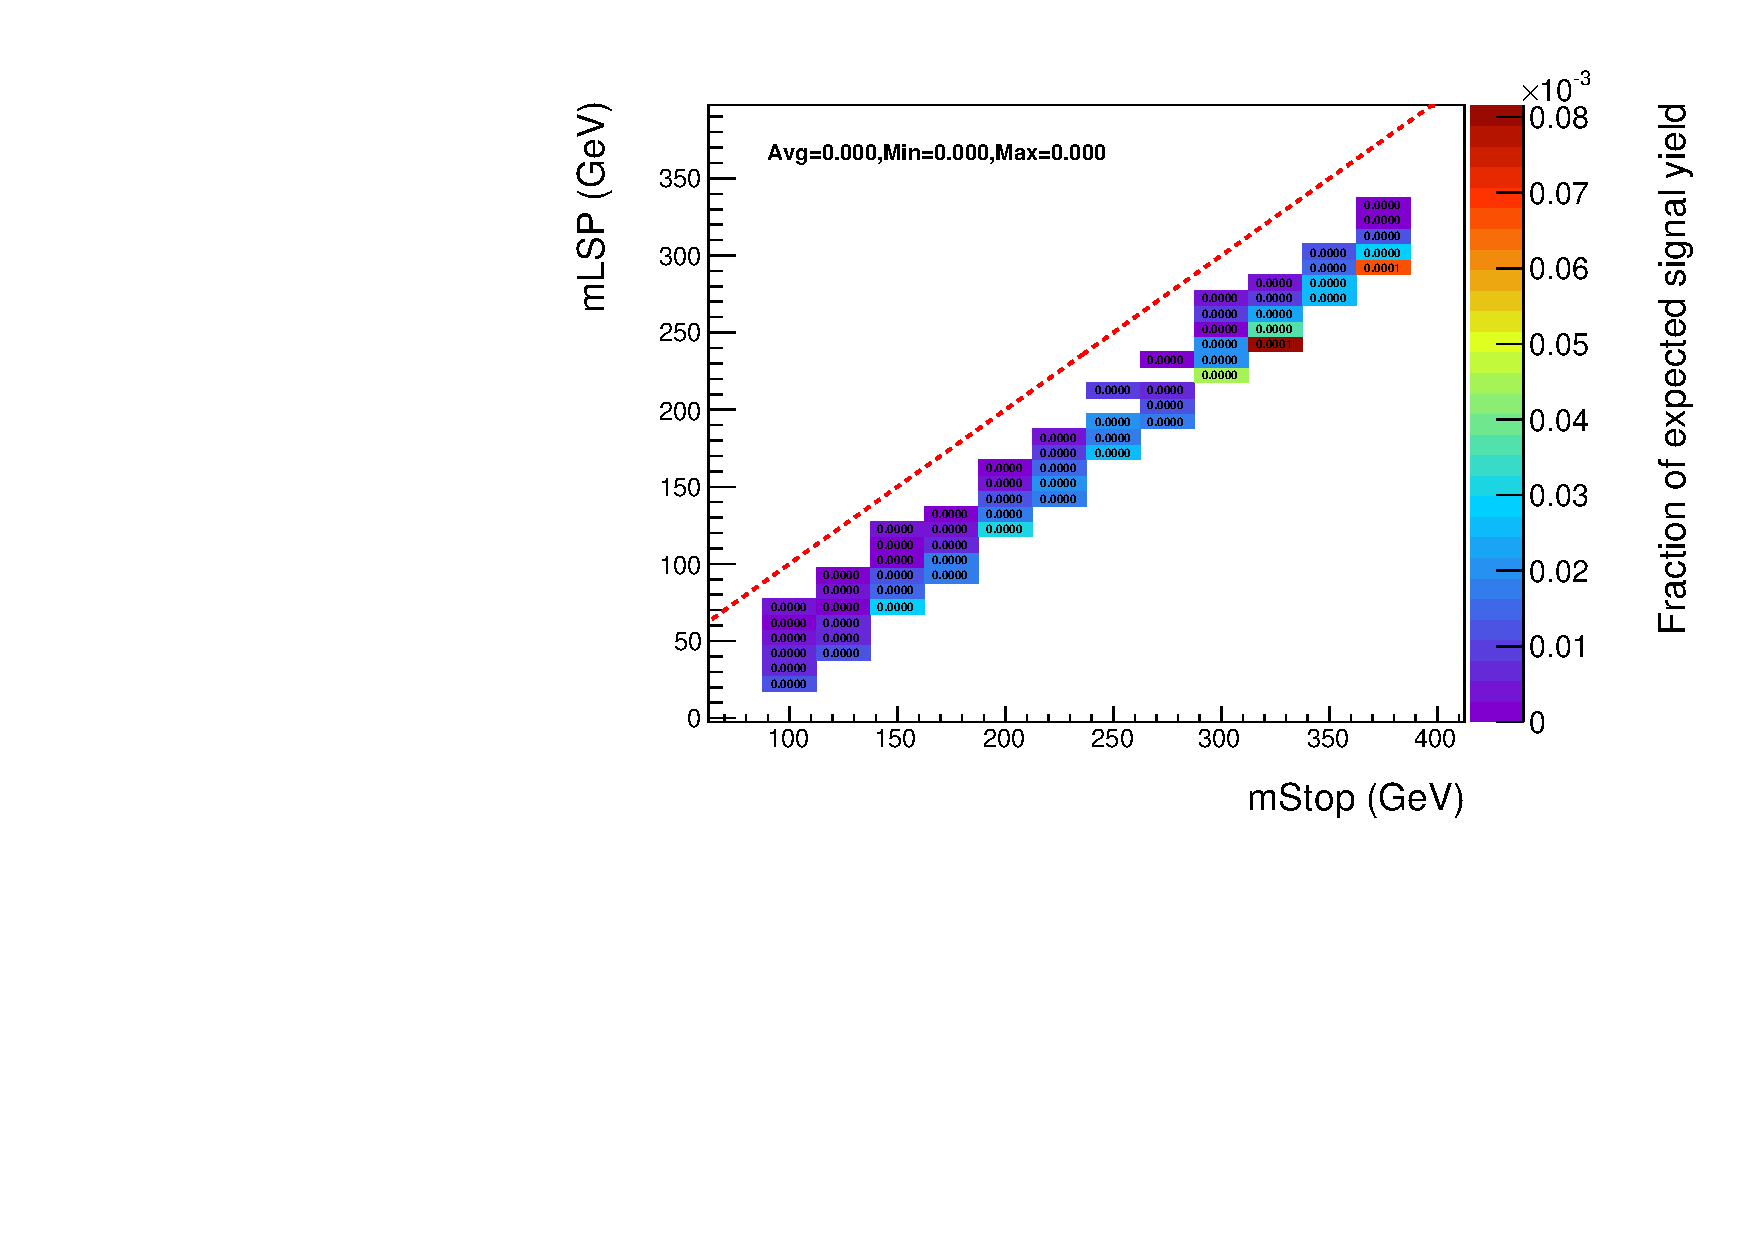
\includegraphics[width=0.4\textwidth]{figures/sms/t2_4body/v16/T2_4body_muon_eff_maps_eq1b_ge4j_SITV}
%    } \\
%    \caption{Signal efficiency times acceptance for the \texttt{T2\_4body}
%      in (left) the signal region and (right) the \mj control sample
%      (\ie, signal contamination) for the relevant event categories
%      defined by \nj and \nb. Note the different z-axis scales.}
%    \label{fig:sms-eff-t2_4body}
%  \end{center}
% \end{figure}

%********************************** % Second Section  *************************************
\section{Systematic Uncertainties on Signal Acceptance }  %Section - 1.2
\label{sec:interpretation_uncertainties}

Due to the reliance on MC simulation for signal model interpretations, a range
of sources of systematic uncertainty on the acceptance times signal efficiency
are considered for each signal 
model. For the main sources, namely jet energy scale (JES), initial state 
radiation (ISR), btag scale factors, parton distribution function (PDF), the 
\mhtmet cut and the dead ECAL filter, systematic values are determined per point
in the scan plane, as a function of \HT, \nb and \nj. The remaining systematics 
are applied as a flat contribution across the entire plane, considered as a 
conservative approach.

Although systematics are considered as a function of the \HT dimension of the 
analysis, all plots shown represent an inclusive selection of \HT>200\gev.

\subsection{Jet energy scale}
The acceptance efficiency is tested for sensitivity to jet energies by measuring
it's change to an upwards and downwards variations of all jet energies by the 
\Pt and $\eta\text{-dependent}$ jet energy scale (JES) uncertainty, as prescribed by 
the JetMET POG.

Distributions showing the acceptance changes due to the variations in JES are 
shown in sections \ref{sec:t2cc_jes_plots} for the \texttt{T2cc} model and
\ref{sec:t2degen_jes_plots} for the \texttt{T2Degen} model.

In both models, the effects of applying 
JES variations are stronger in the \njhigh category. An increased number of jets
sharing the small kinematic phase space of the compressed region implies softer jets.
Therefore applying
variations on the jet energies is more likely to move jets in and out of 
acceptance. This effect is also noticeable in the \njlow, 1b category for 
\texttt{T2cc} (figure~\ref{fig:sms-jes-t2cc-le3j-1b}), where changes in acceptance
are larger away from the diagonal, 
where acceptance is dependent on jets originating from the soft SUSY decay.

The \texttt{T2Degen} model decay contains a real b-quark, and consequently JES 
uncertainties have a dependence on \nb, where higher variations are observed in 
the \nb=1 category (figure~\ref{fig:sms-jes-tdegen-le3j-1b}).


\subsection{Initial State Radiation}
As described in section~\ref{sec:isr_reweighting}, boost \Pt dependent 
event weights are taken from the data to MC comparison study performed within
the SUSY PAG. A procedure is also defined to determine related systematics, by
applying upwards and downwards variations of weights corresponding to the 
magnitude of the corrections themselves, and studying the effect on signal 
efficiency times acceptance. These weights are summarised in
table~\ref{tab:isr_syst_weights}.

\begin{table}[ht!]
  \caption{Systematic factors for \MADGRAPH based signal samples to determine 
  ISR modelling related systematics.\label{tab:isr_syst_weights}}
  \centering
  \small
  \begin{tabular}{ lc }
    \hline
    \hline
    $\Pt_{boost} (\gev)$         & Systematic Variation \\
    \hline
    $0 <\Pt\leq120    $          & $\pm0.0$ \\
    $120 <\Pt\leq150  $          & $\pm0.05$ \\
    $150 <\Pt\leq250  $          & $\pm0.10$ \\
    $250 < \Pt        $          & $\pm0.20$ \\    
    \hline
    \hline
  \end{tabular}
\end{table}

As discussed previously in sections~\ref{sec:t2cc_eff} and \ref{sec:t2degen_eff},
acceptance for compressed spectra models at the smallest \deltam (i.e. nearest 
the diagonal) is almost entirely due to presence of hard ISR jets. Away from the
diagonal, ISR jets are still important, however they are relied upon to boost 
the soft SUSY decay system. Subsequently, systematics due to ISR variations are 
observed to be largest nearest the diagonal for all categories, as shown in
figure~\ref{fig:sms-isr-t2cc} and \ref{fig:sms-isr-t2degen} for \texttt{T2cc} 
and \texttt{T2Degen} respectively. Due to this dependence, systematics related 
to ISR are the largest contribution.


\subsection{Btag scale factors}
Specifically for \FASTSIM signal samples, events are not weighted using the 
b-tag formula method described in section (REF), but instead using the 
recommended method for \FULLSIM samples with an additional \FULLSIM to \FASTSIM 
correction factor applied. The original correction is dependent on the generator
level content of an event, and is defined as:

\begin{equation}
w = \frac{SF_b \epsilon \times (1-SF_b \epsilon) \times SF_{c,light} m \times (1
-SF_{c,light} m)}{\epsilon \times (1-\epsilon) \times m \times (1-m)}
\label{eq:btag_fullsim_weight}
\end{equation}

where $\epsilon(\Pt, \eta)$ and $m(\Pt, \eta)$ are the b-tagging efficiency and 
mistagging rate, respectively. These factors are functions of \Pt and $\eta$, and
are measured in SM MC for both the hadronic and \mj samples, for each \HT bin.

Applying this event weight provides `corrected MC yields', which are then 
have further \FASTSIM to \FULLSIM correction factors applied, as defined by REF 
AN-2012-175.

Systematic variations equal to the errors of these corrections are applied as 
upwards and downwards deviations, and any effects on signal efficiency times 
acceptance are studied.

As expected, only small changes in acceptance are found in the \texttt{T2cc} 
model when btag scale factor variations are applied, as shown in
figure~\ref{sec:t2cc_btag_plots}. While not entirely negligible, it is worth 
noting that systematics are slightly larger for the \nb=1 category
(figure~\ref{fig:sms-btag-t2cc-le3j-1b}), however still at a low level with 
respect to other systematic sources.

The \texttt{T2Degen} model, containing a real b-quark, has WHAT?
WHY IS T2DEGEN AT THE SAME LEVEL AS T2CC?! IS THAT CORRECT?


\subsection{PDF}
Signal samples are produced using the \textsc{CTEQ6L1} PDF set. The acceptance 
sensitivity to the used PDF set is investigated by comparing results using three
other commonly used PDF sets, namely \textsc{CT10}, \textsc{NNPDF2.1} and
\textsc{MSTW2008}. Following PDF4LHC recommendations [REF], the output is 
combined to determine an `envelope' value combining the three alternative PDF 
sets, and a related systematic uncertainty.

\emph{T2cc plots and some observations}

\emph{T2degen plots and some observations}

\subsection{MHT/MET cleaning cut}
\label{sec:mhtmet_syst}
The efficiency of the \mhtmet cleaning cut is compared between data and MC with 
the aim of revealing any potential issues due to MC mis-modelling of the 
variable. Efficiencies are compared in the \mj control sample, using \HT bins 
ranging from $200 < \HT < 375 \gev$, in both \nj categories, with no requirement
on \nb. Efficiencies are summarised in table~\ref{tab:mht-met}, where 
efficiency comparisons between data and MC statistically agree with unity.

\emph{this covers \FULLSIM and data agreement, but what do we do for \FASTSIM to 
\FULLSIM agreement?}

\begin{table}[!h]
  \caption{Efficiencies for the requirement $\mhtmet < 1.25$ obtained
    from data ($\epsilon_{\text{data}}$) and simulation
    ($\epsilon_{\text{MC}} $) in the \mj control sample with an
    inclusive selection on \nb, the requirement $\alphat > 0.55$, for
    the analysis bins at low \HT, and for the two jet multiplicity
    bins, \njlow and \njhigh. Also quoted are the ratios of these
    efficiencies ($\epsilon_{\text{MC}}/\epsilon_{\text{data}}$),
    which is representative of the simulation performance with respect
    to the \mht/\met variable. REWORD 
  }
  \label{tab:mht-met}
  \centering
  \footnotesize
  \begin{tabular}{ ccccc }
    \hline
    \hline
    \nj    & \HT (GeV) & $\epsilon_{\text{MC}}$ & $\epsilon_{\text{data}}$ & $\epsilon_{\text{MC}}/\epsilon_{\text{data}}$ \\
    \hline
    2--3     & 200--275      & $0.95 \pm 0.00$        & $0.95 \pm 0.01$          & $1.00 \pm 0.01$                               \\
    2--3     & 275--325      & $0.97 \pm 0.01$        & $0.97 \pm 0.02$          & $1.00 \pm 0.02$                               \\
    2--3     & 325--375      & $0.97 \pm 0.01$        & $0.97 \pm 0.02$          & $1.00 \pm 0.02$                               \\
    2--3     & 375--475      & $0.98 \pm 0.01$        & $0.98 \pm 0.03$          & $1.00 \pm 0.03$                               \\
    $\geq 4$ & 200--275      & $0.90 \pm 0.02$        & $0.92 \pm 0.04$          & $0.98 \pm 0.04$                               \\
    $\geq 4$ & 275--325      & $0.92 \pm 0.01$        & $0.93 \pm 0.02$          & $0.99 \pm 0.02$                               \\
    $\geq 4$ & 325--375      & $0.92 \pm 0.01$        & $0.93 \pm 0.04$          & $0.99 \pm 0.04$                               \\
    $\geq 4$ & 375--475      & $0.95 \pm 0.02$        & $0.95 \pm 0.04$          & $1.00 \pm 0.04$                               \\
    \hline
    \hline
  \end{tabular}
\end{table}

\emph{T2cc plots and some observations}

\emph{T2degen plots and some observations}

\subsection{Dead ECAL Filter}
To assess any potential MC mis-modelling issues with the dead ECAL filter, a 
similar analysis is made as described in section~\ref{sec:mhtmet_syst}. 
Efficiencies between data and MC are compared for the \mj selection, with an 
inclusive requirement on both \nb and \HT. As shown in table~\ref{tab:dead-ecal},
the ratio of efficiencies between data and MC for each \nj category agree within
statistical errors.

\emph{\FULLSIM to \FASTSIM systs?}

\begin{table}[!h]
  \caption{Efficiencies of the dead ECAL cut for the \mj selection in data and 
  MC. Inclusive requirements are made of \nb and \HT.}
  \label{tab:dead-ecal}
  \centering
  \footnotesize
  \begin{tabular}{ ccccc }
  % \begin{tabular}{ ccc }
    \hline
    \hline
    \nj    & \HT (GeV) & $\epsilon_{\text{MC}}$ & $\epsilon_{\text{data}}$ & $\epsilon_{\text{MC}}/\epsilon_{\text{data}}$ \\
    % \nj     & \HT (GeV) & $\epsilon_{\text{MC}}/\epsilon_{\text{data}}$                                                     \\
    \hline
    2--3     & $>200$        & $0.64 \pm 0.01$        & $0.64 \pm 0.01$          & $1.00 \pm 0.01$                               \\
    $\geq 4$ & $>200$        & $0.58 \pm 0.01$        & $0.59 \pm 0.01$          & $0.98 \pm 0.01$                               \\
    % 2--3      & $>200$        & $1.00 \pm 0.01$                                                                                   \\
    % $\geq 4$  & $>200$        & $0.98 \pm 0.01$                                                                                   \\
    \hline
    \hline
  \end{tabular}
\end{table}

\emph{T2cc plots and some observations}

\emph{T2degen plots and some observations}

\subsection{Generator Level Partons}
At the \MADGRAPH matrix element stage of the MC simulation production, a number
of additional feynman diagrams are simulated to account for associated parton 
interactions, such as ISR and FSR. Given the dependence on such processes in the
compressed spectra regime, an additional sub-sample of the \texttt{T2cc} scan 
has been produced with up to 3 additional partons, to compare against the 
complete scan's up to 2 additional partons. This scan contains two mass points 
at a stop mass near the region of maximum sensitivity, with mass splittings 
covering the entire range of the scan. The relative change in efficiency times 
acceptance between the two scans is shown in table~\ref{tab:sms-t2cc-2v3part}. 
These values are interpretted as systematic uncertainties on the number of 
associated partons modelled for such compressed spectra models, and are applied 
as flat contributions across the scan plan for all models.

\begin{table}[!h]
  \caption{Relative change in efficiency times acceptance for the
    2-parton and 3-parton scans in the signal region, with an inclusive 
    selection on \nb and \HT>200 \gev. The scan points are $m_{\sTop} = 200$ \gev 
    and $m_{\chiz} = (120, 190)$ \gev.}
  \label{tab:sms-t2cc-2v3part}
  \centering
  \small
  \begin{tabular}{ lcc }
    \hline
    \hline
    Category     & \multicolumn{2}{c}{$\Delta m$ (GeV)} \\
    \cline{2-3}
                 & 10   & 80                            \\
    \hline
    (2--3,0)     & 0.00 & 0.04                          \\
    (2--3,1)     & 0.02 & 0.04                          \\
    ($\geq 4$,0) & 0.04 & 0.04                          \\
    ($\geq 4$,1) & 0.00 & 0.00                          \\
    \hline
    \hline
  \end{tabular}
\end{table}


\subsection{Luminosity Measurement}
Flat corrections across the scan plane are made to account for the uncertainty 
of the luminosity measurement, as quoted by Lumi POG at 2.3\% [REF].

\subsection{Summary}

For each mass point in the scan plane, the total systematic is the sum in 
quadrature of all individual contributions. Summaries are shown in
tables~\ref{tab:sms-syst-t2cc} and \ref{tab:sms-syst-t2_4body}.

\emph{NOTE: these values are all placeholders and need to be scrutinised!}

\begin{table}[h!]
  \caption{Representative ranges for each contribution to the total
    systematic uncertainty in the signal efficiency times acceptance
    for each relevant event category for the \texttt{T2cc}
    interpretation. See text for further details on other
    (fixed) contributions to the total systematic uncertainty. REWORD 
    \label{tab:sms-syst-t2cc}
  }   
  \centering
  \small
  \begin{tabular}{ lcccccccc }
    \hline
    \hline
    Category   & \multicolumn{2}{c}{(2--3,0)} & \multicolumn{2}{c}{($\geq 4$,0)} & \multicolumn{2}{c}{($\geq 4$,1)} & \multicolumn{2}{c}{($\geq 2$,$\geq 0$)} \\
    Range      & Min.                         & Max.                             & Min.                             & Max. & Min. & Max. & Min. & Max.        \\
    \hline
    PDF        &                              &                                  &                                  &      &      &      & 0.04 & 0.14        \\
    JES        & 0.00                         & 0.08                             & 0.06                             & 0.22 & 0.01 & 0.30 &      &             \\
    ISR        & 0.09                         & 0.21                             & 0.16                             & 0.24 & 0.15 & 0.24 &      &             \\
    b-tag SF   & 0.01                         & 0.02                             & 0.01                             & 0.02 & 0.03 & 0.04 &      &             \\
    \mhtmet    & 0.02                         & 0.02                             & 0.02                             & 0.02 & 0.02 & 0.02 &      &             \\
    Dead ECAL  & 0.02                         & 0.02                             & 0.02                             & 0.02 & 0.02 & 0.02 &      &             \\
    \hline
    Total syst & 0.12                         & 0.21                             & 0.22                             & 0.32 & 0.23 & 0.39 &      &             \\
    \hline
    \hline
  \end{tabular}
\end{table}

\begin{table}[h!]
  \caption{Representative ranges for each contribution to the total
    systematic uncertainty in the signal efficiency times acceptance
    for each relevant event category for the \texttt{T2Degen}
    interpretation. See text for further details on other
    (fixed) contributions to the total systematic uncertainty. REWORD
    \label{tab:sms-syst-t2_4body}
  }   
  \centering
  \small
  \begin{tabular}{ lcccccccc }
    \hline
    \hline
    Category   & \multicolumn{2}{c}{(2--3,0)} & \multicolumn{2}{c}{($\geq 4$,0)} & \multicolumn{2}{c}{($\geq 4$,1)} & \multicolumn{2}{c}{($\geq 2$,$\geq 0$)} \\
    Range      & Min.                         & Max.                             & Min.                             & Max. & Min. & Max. & Min. & Max.        \\
    \hline
    PDF        &                              &                                  &                                  &      &      &      & 0.04 & 0.14        \\
    JES        & 0.00                         & 0.08                             & 0.06                             & 0.22 & 0.01 & 0.30 &      &             \\
    ISR        & 0.09                         & 0.21                             & 0.16                             & 0.24 & 0.15 & 0.24 &      &             \\
    b-tag SF   & 0.01                         & 0.02                             & 0.01                             & 0.02 & 0.03 & 0.04 &      &             \\
    \mhtmet    & 0.02                         & 0.02                             & 0.02                             & 0.02 & 0.02 & 0.02 &      &             \\
    Dead ECAL  & 0.02                         & 0.02                             & 0.02                             & 0.02 & 0.02 & 0.02 &      &             \\
    \hline
    Total syst & 0.12                         & 0.21                             & 0.22                             & 0.32 & 0.23 & 0.39 &      &             \\
    \hline
    \hline
  \end{tabular}
\end{table}


%********************************** % Third Section  *************************************
\section{Limits on models of Supersymmetry}  %Section - 1.3
\label{sec:interpretation_limits}

\subsection{Overview of limit setting procedure}
Using green and blue band fits for expected and observed
considering MC stats of signal MC samples
point-by-point systematics

discussion of CLs method. Look up `CLs 4 LHC'

\subsection{Limits}
different limits for the various models


%********************************** % Fourth Section  *************************************
\section{Interpretation of excesses}
\label{sec:interpretation_excess}
best fit points in T2cc
global context?
p-values with SUSY assumption? is that even a thing? who knows? who cares.